\documentclass[a4paper]{article}        % Standaard een kolom layout
\usepackage[english]{babel}               % Stel woordafbrekingen en referentienamen in
\usepackage{graphicx}                   % Afbeeldingen weergeven
\usepackage{float}                      % Figuren op plaats waar ze gedefinieerd staan: [H]
\usepackage{lmodern}                    % Gebruik modern lettertype
\usepackage[T1]{fontenc}
\usepackage[hidelinks]{hyperref}        % Referenties aanklikbaar in PDF, geen kaders rond weergeven
\usepackage[margin=1.5in]{geometry}
\usepackage[binary-units,per-mode=symbol]{siunitx}                    % SI unit symbolen
\usepackage{amsmath}                    % Matrices en vergelijkingen
\usepackage{subcaption}                 % Subfiguren
\usepackage{tabularx}
\usepackage[parfill]{parskip}
\DeclareSIUnit\dbm{\decibel{}m}         % Voeg dBm toe als eenheid
\usepackage{tikz}
\usetikzlibrary{shapes,arrows}
\usepackage{csvsimple}
\usepackage{hyperref}
\usepackage{natbib}


\title{High Frequency Design: \\ Design of an RF front-end for a GPS receiver}
\author{Thomas Deckmyn \& Zeger Van de Vannet}
\date{\today}
\begin{document}
\maketitle

\tableofcontents

\section{Introduction}
\section{Circuit Design}
	\subsection{LNA}

	\textbf{Misschien specificaties nog eens oplijsten?}\\\\
	The design of the LNA first requires a choice of topology. A common emittor toplogy is the best choice in this case, because it yields the highest power gain and has a moderate input and output impedance, hence it can easily be matched to a $\SI{50}{\ohm}$ system.
		\subsubsection{DC Operating Point}
			When determining the DC operating point for the BFP740 transistor a trade-off has to be made between minimal NF and maximum linearity. Based on the characteristics found in the datasheet\cite{transdatasheet} of the transistor we choose $V_{CE} = \SI{4}{\volt}$ and $I_C = \SI{20}{\milli\ampere}$ to obtain the highest possible linearity, i.e. $IP3 = \SI{27}{\dbm} $. For $I_C = \SI{20}{\milli\ampere}$ the NF is $\SI{0.7}{\decibel}$, which still leaves a lot of margin to stay below the specified NF of $\SI{1.5}{\decibel}$. From the datasheet we know that $\beta = 300$, which yields $I_B = \frac{I_C}{\beta} = \SI{66}{\micro\ampere}$, hence the circuit shown in Figure \ref{fig:lna_ce} can be constructed. DC blocking capacitor are added as not to interrupt the DC operating point of the transistor. The DC feed ensures DC current where needed and prevents RF current from entering the DC voltage source. \\

			\begin{figure}[H]
			\centering
				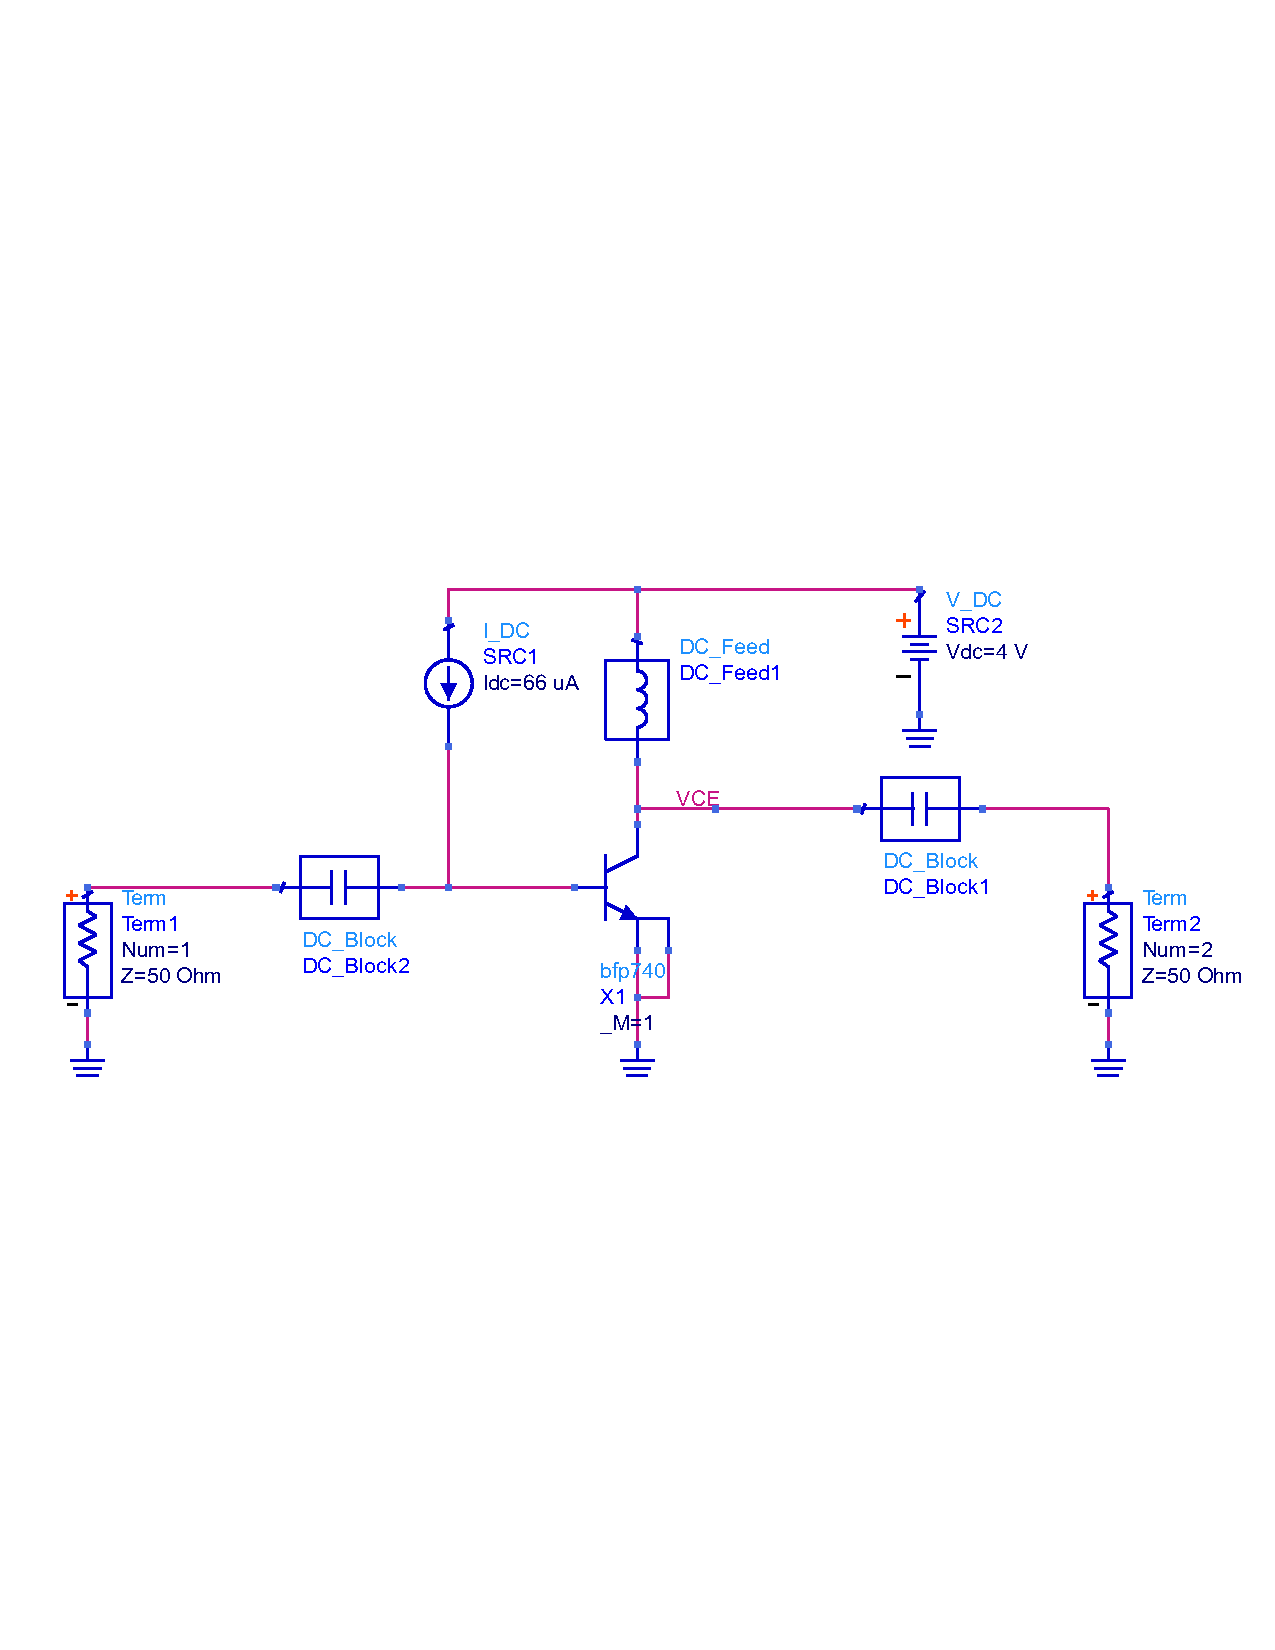
\includegraphics[width=0.8\textwidth]{fig/LNA/LNA_start.pdf}
			\caption{Common emitter topology}
			\label{fig:lna_ce}
			\end{figure}

			To enable the $\SI{5}{\volt}$ supply the DC feed can be replaced by a resistor, which will lower the collecor emittor voltage. We want $I_C$ to still be $\SI{20}{\milli\ampere}$ and $V_{CE}$ $\SI{4}{\volt}$. This means we need a $\SI{1}{\volt}$ voltage drop over the resistor and $\SI{20}{\milli\ampere}$ going through it, hence $R = \frac{V}{I} = \SI{50}{\ohm}$. We obtain the circuit in Figure \ref{fig:lna_5V}.

			\begin{figure}[H]
			\centering
				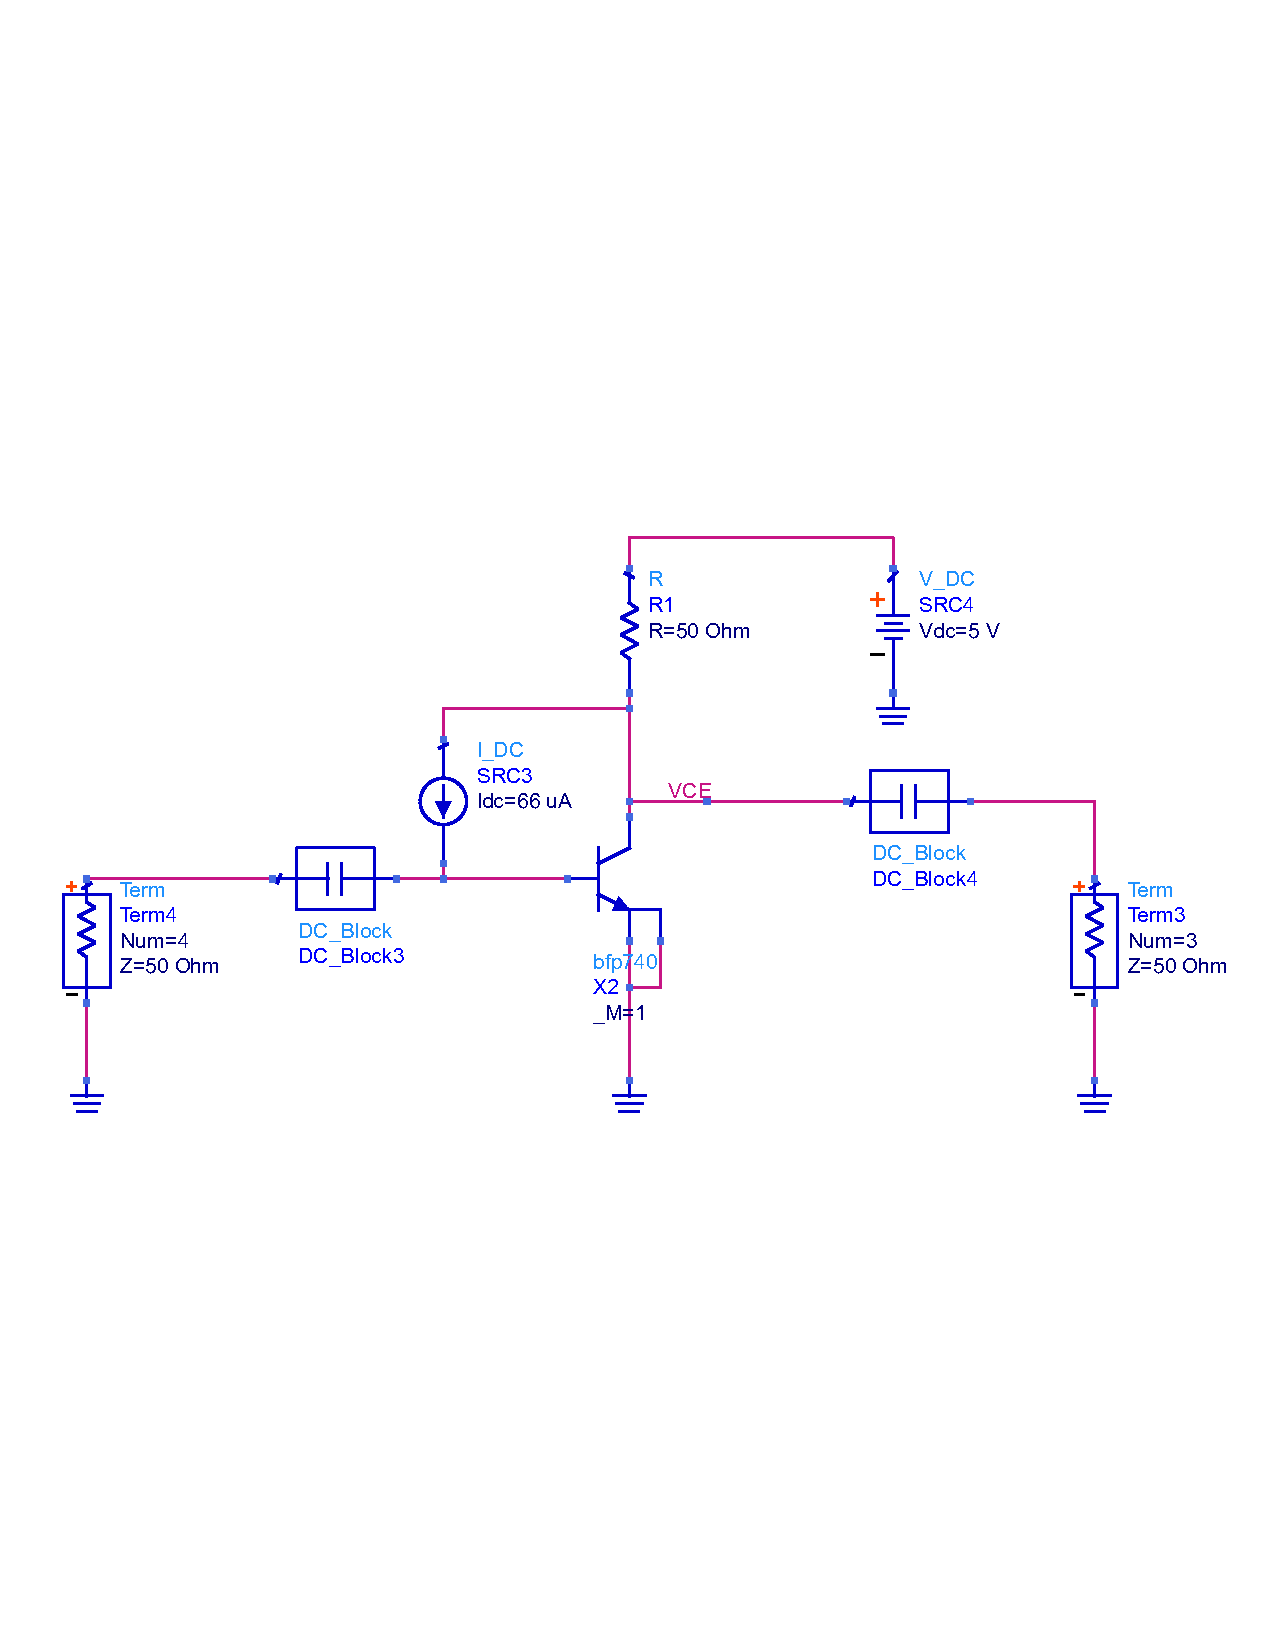
\includegraphics[width=0.8\textwidth]{fig/LNA/LNA_5V.pdf}
			\caption{DC feed replaced with resistor enabling 5V supply}
			\label{fig:lna_5V}
			\end{figure}

		\subsubsection{Stability}
			To decide wether the amplifier is stable, we draw the input and output stability circles. We know that in the center of the Smith Chart $\Gamma_{in} = |S_{11}] < 1$ and $\Gamma_{out} = |S_{22}| < 1$, hence if the stability circles do not intersect with the unity circle the amplifier is stable for all possible passive terminations at the design frequency.\cite{pozar} The value of the stability resistor(s) tunes diameter and position of the stability circle, hence stability can be obtained by tuning the resistor(s).\\

			 To obtain a stable amplifier there a few choices that can be made concerning the position of the stability resistor, i.e. shunt or series at input or output, or a combination of multiple resistors. As we are designing a low noise amplifier a series resistor at the input would be a bad choice, as this would increase the NF considerably. To stabilize the amplifier with solely a shunt resistance at the input a very high resistance is needed (order of $\SI{100}{\kilo\ohm}$), which would put non realisable constraints on the matching network. After analyzing the two remaining options and combinations, we conclude that best performance with respect to NF and gain is achieved with a series resistance at the output and a shunt resistance at the input. The realized stabilization circuit can be seen in Figure \ref{fig:lna_stable}.

			 \begin{figure}[H]
				\centering
				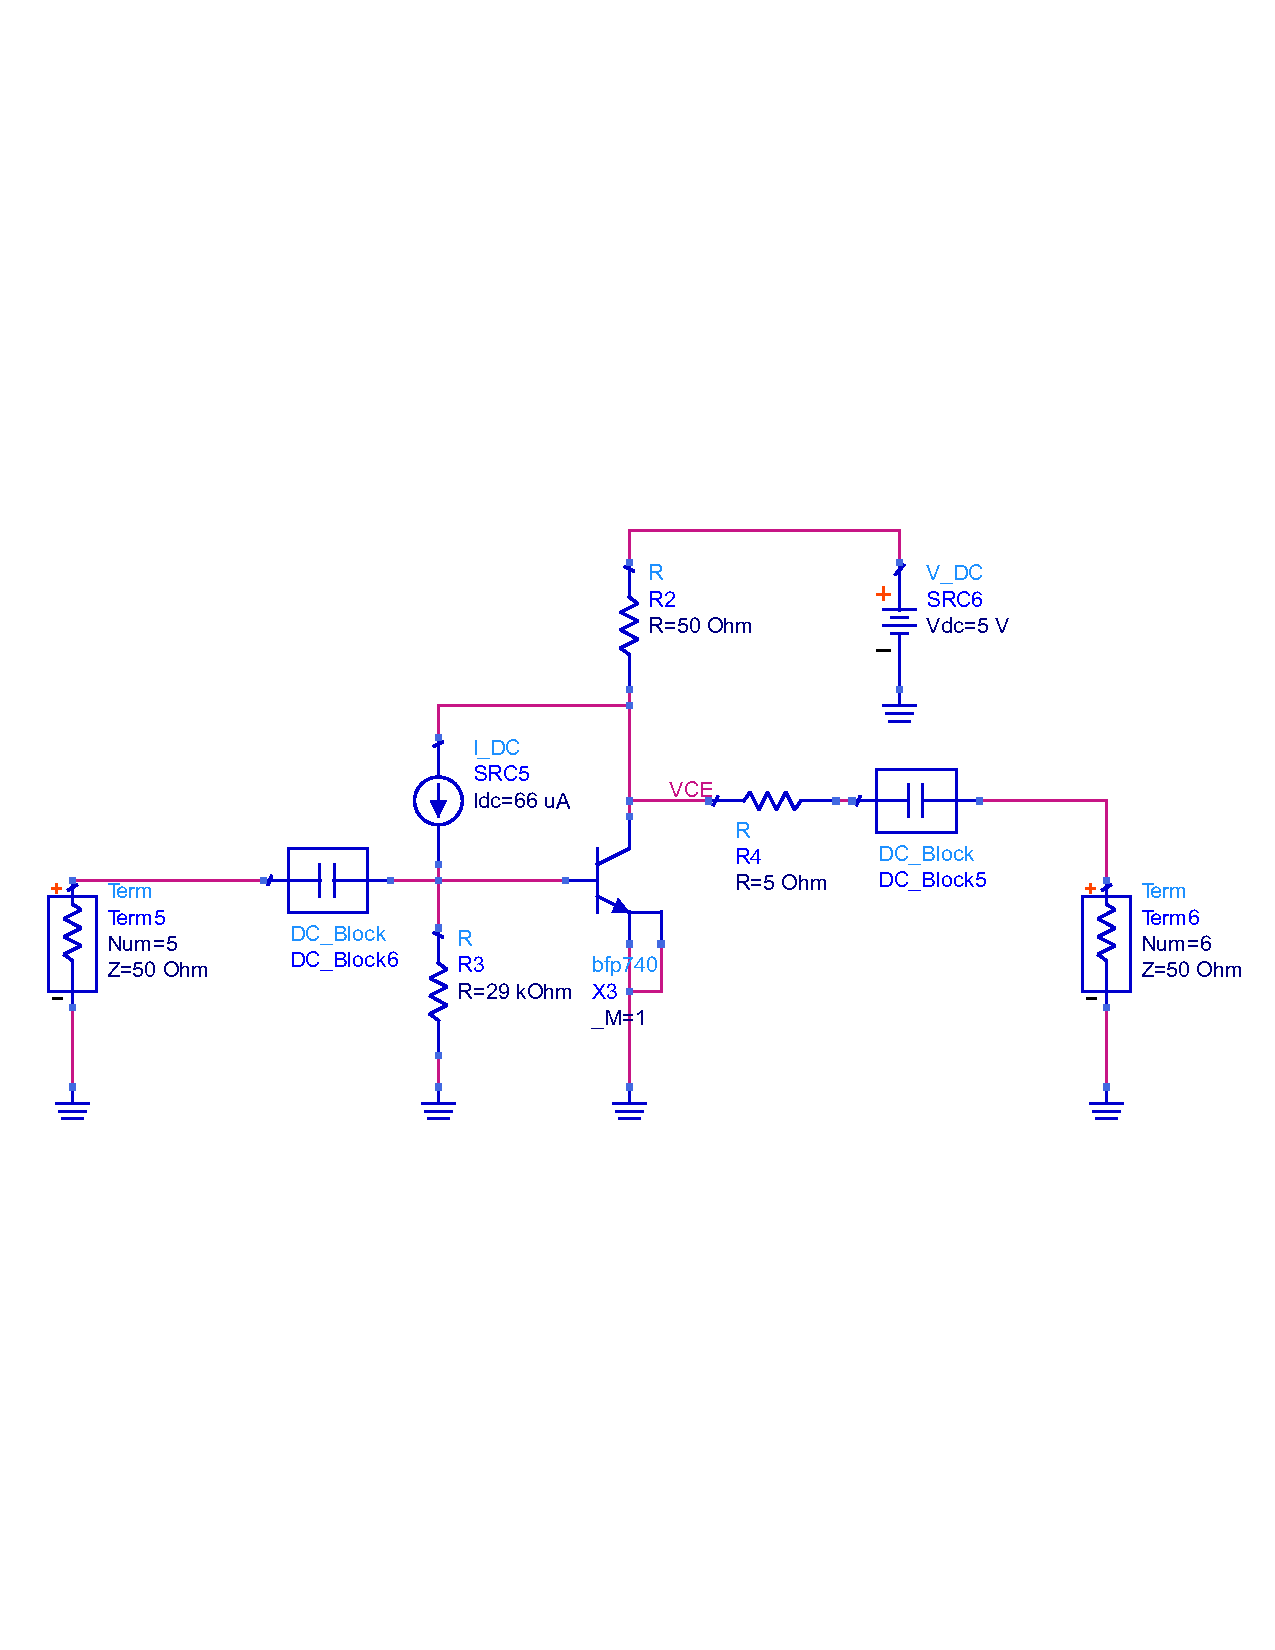
\includegraphics[width=0.8\textwidth]{fig/LNA/LNA_stable.pdf}
				\caption{Circuit for LNA with added stabilization resistors}
				\label{fig:lna_stable}
			\end{figure}

		\subsubsection{Gain and Noise Matching and Biasing}
		\label{sec:lna_matching}

			What is still left to do is selecting the load and source reflection coefficients. For this we draw constant gain circles in the output plane and constant noise circles in the input plane. Next, we choose the load reflection coefficient $\Gamma_L$ in such a way that the source reflection coefficient $\Gamma_S$ is within the constant noise circle of $\SI{1.5}{\decibel}$ as specified. To achieve a NF that is below $\SI{1.5}{\decibel}$ we will need to sacrifice gain at the output, as can be seen in Figure \ref{fig:lna_circles}. The load reflection $\Gamma_L$ is chosen on the $\SI{20}{\decibel}$ gain circle and then the source reflection $\Gamma_S$ is within the $\SI{1.5}{\decibel}$ noise circle. \\

			First, the output is matched such that $\Gamma_L$ is located at $Z_0 (0.645 + j 0.109)$ on the Smith Chart, which will reduce the gain to $\SI{20}{\decibel}$, but the NF will be within the specifications. Second, the input impedance is matched to $\SI{50}{\ohm}$. The matching is performed using the Smith Chart Tool in ADS and both networks consist of a piece of transmission line and a capacitor. The circuit with the added matching networks is shown in Figure \ref{fig:lna_pre_layout}. The DC blocks can be omitted as the capacitors of the matching network now act as DC blocks. 

			\begin{figure}[H]
			\begin{subfigure}{0.5\textwidth}
				\centering
				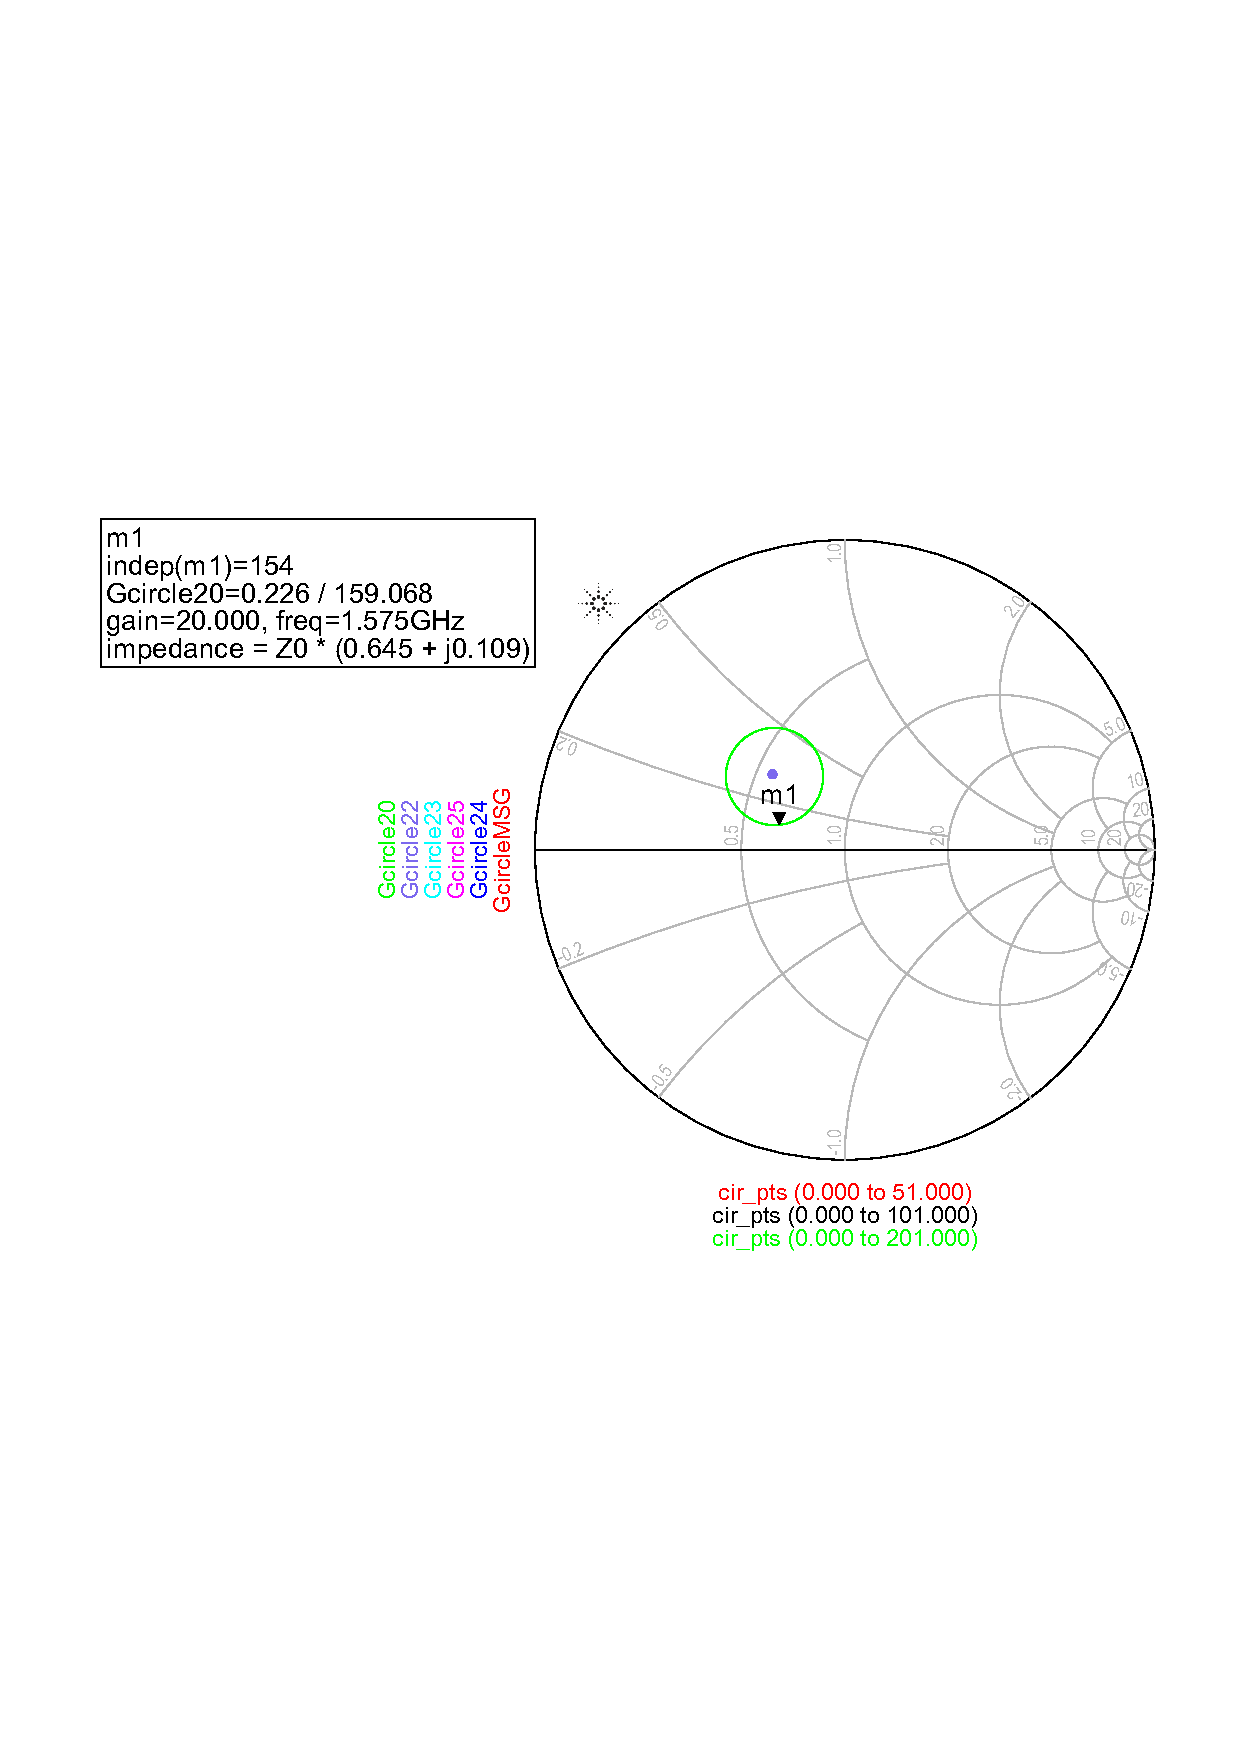
\includegraphics[width=\textwidth]{fig/LNA/LNA_gain_circle.pdf}
			\end{subfigure}
			\begin{subfigure}{0.5\textwidth}
				\centering
				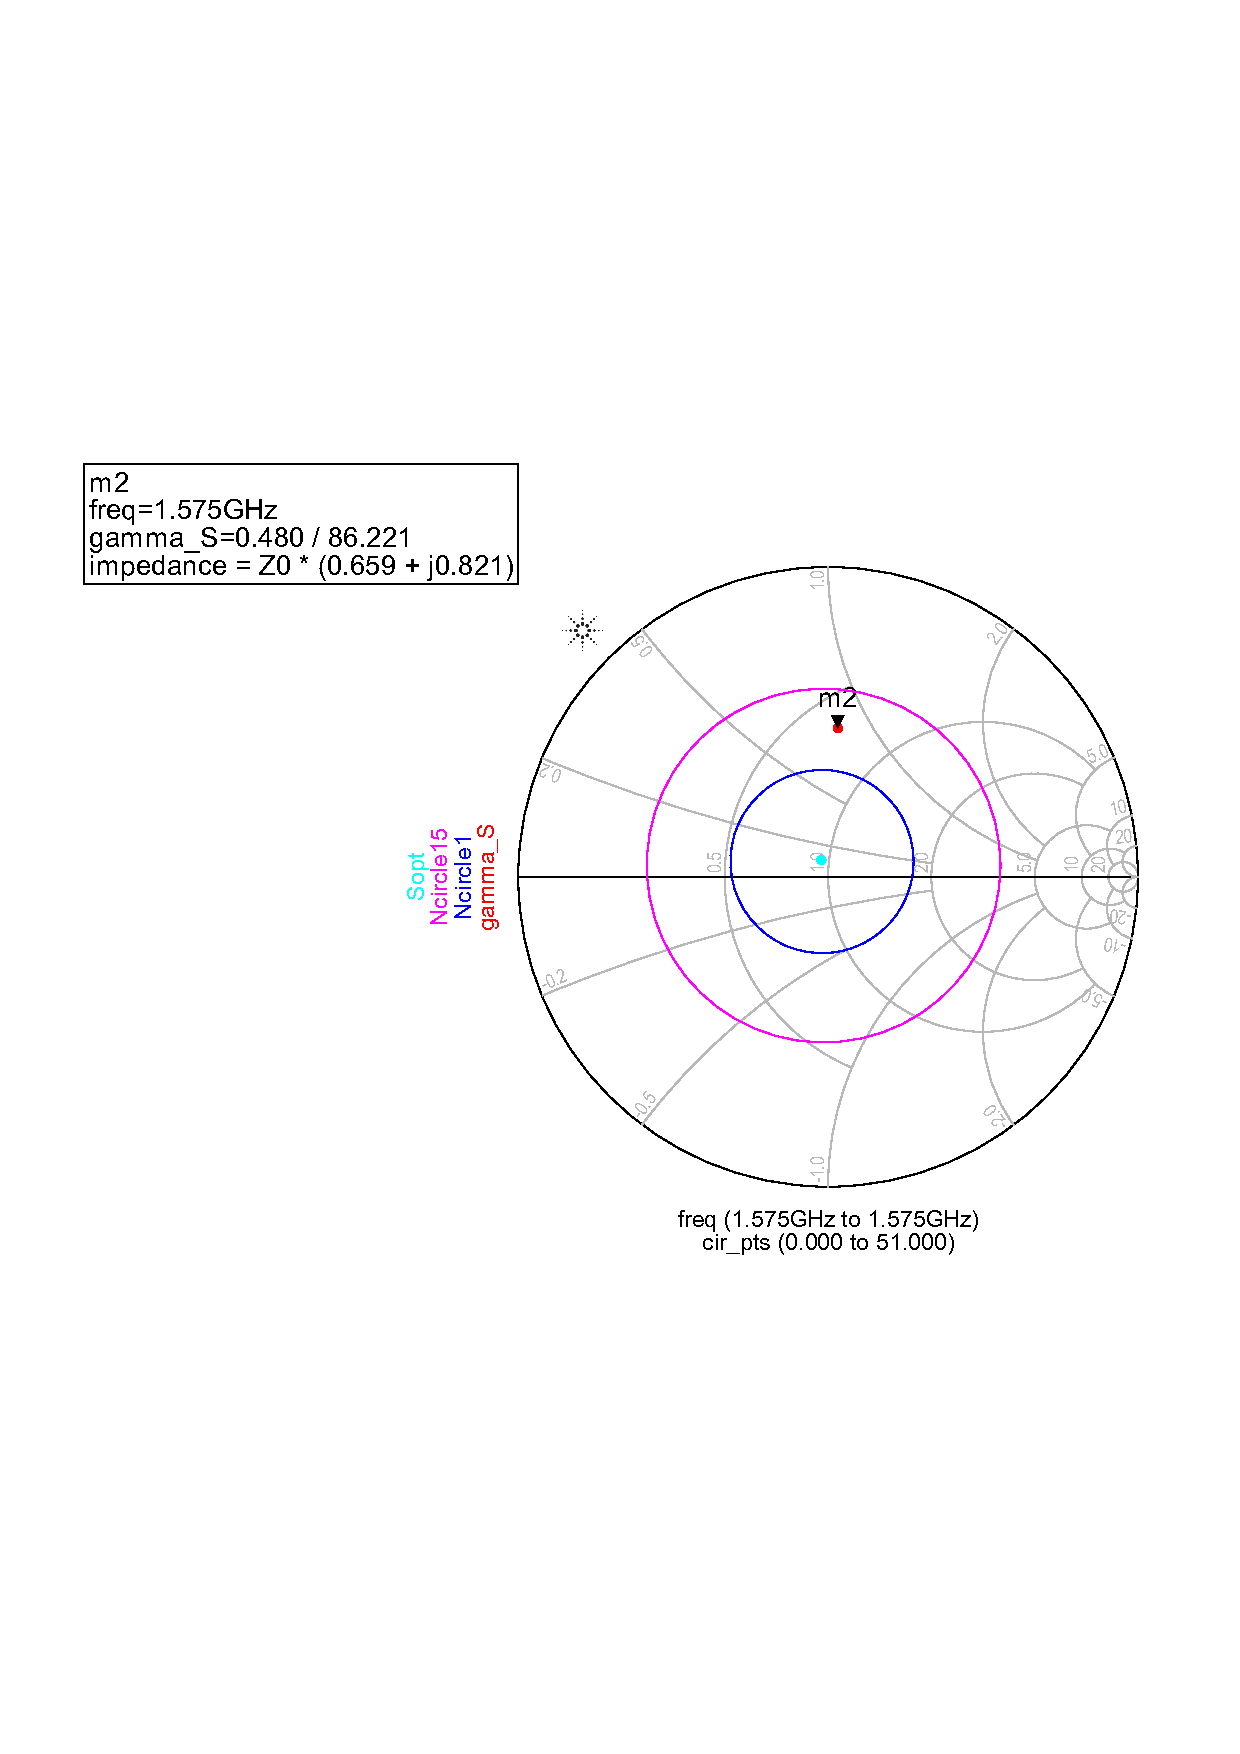
\includegraphics[width=\textwidth]{fig/LNA/LNA_noise_circle.pdf}
			\end{subfigure}
				\caption{Constant Noise and Gain circles for matching}
				\label{fig:lna_circles}
			\end{figure}

			The next step is to replace the ideal base current source by a biasing network. This biasing network will induce negative feedback and thus ensure stability. The voltage drop over the resistor will be $V_{CE} - \SI{0.7}{\volt} = \SI{3.3}{\volt}$ and the current needs to be $\SI{66}{\micro\ampere}$, hence $R = \SI{50}{\kilo\ohm}$. After tuning for best performance, we obtain the circuit shown in Figure \ref{fig:lna_pre_layout}.

			\begin{figure}[H]
				\centering
				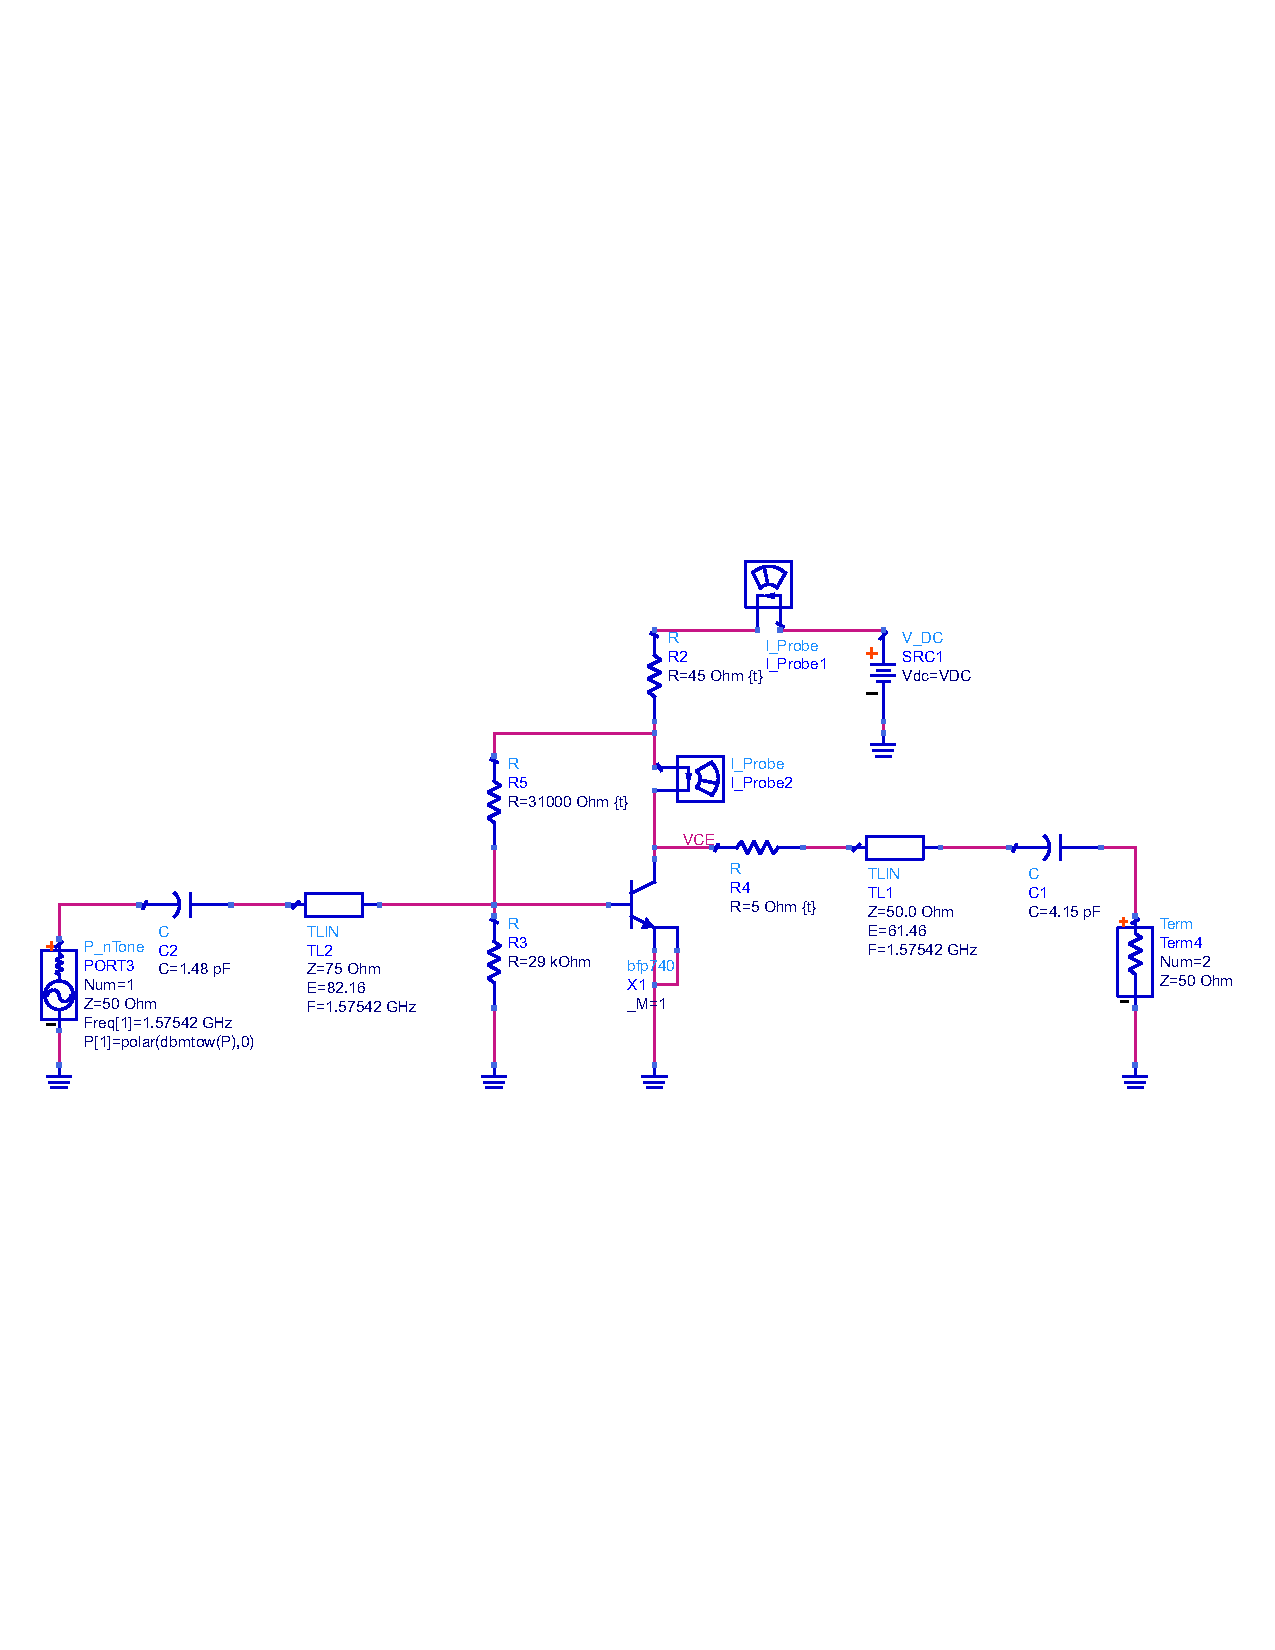
\includegraphics[width=0.8\textwidth]{fig/LNA/LNA_matched.pdf}
			\caption{Realized circuit after matching and biasing}
			\label{fig:lna_pre_layout}
			\end{figure} 

			The Smith Chart in Figure \ref{fig:lna_matching_smith} shows that the input is perfectly matched to $\SI{50}{\ohm}$ after adding the matching networks from Figure \ref{fig:lna_pre_layout}. The output is on purpose mismatched to obtain a NF that is smaller than $\SI{1.5}{\decibel}$ (see \ref{sec:lna_matching}).

			\begin{figure}[H]
			\centering
				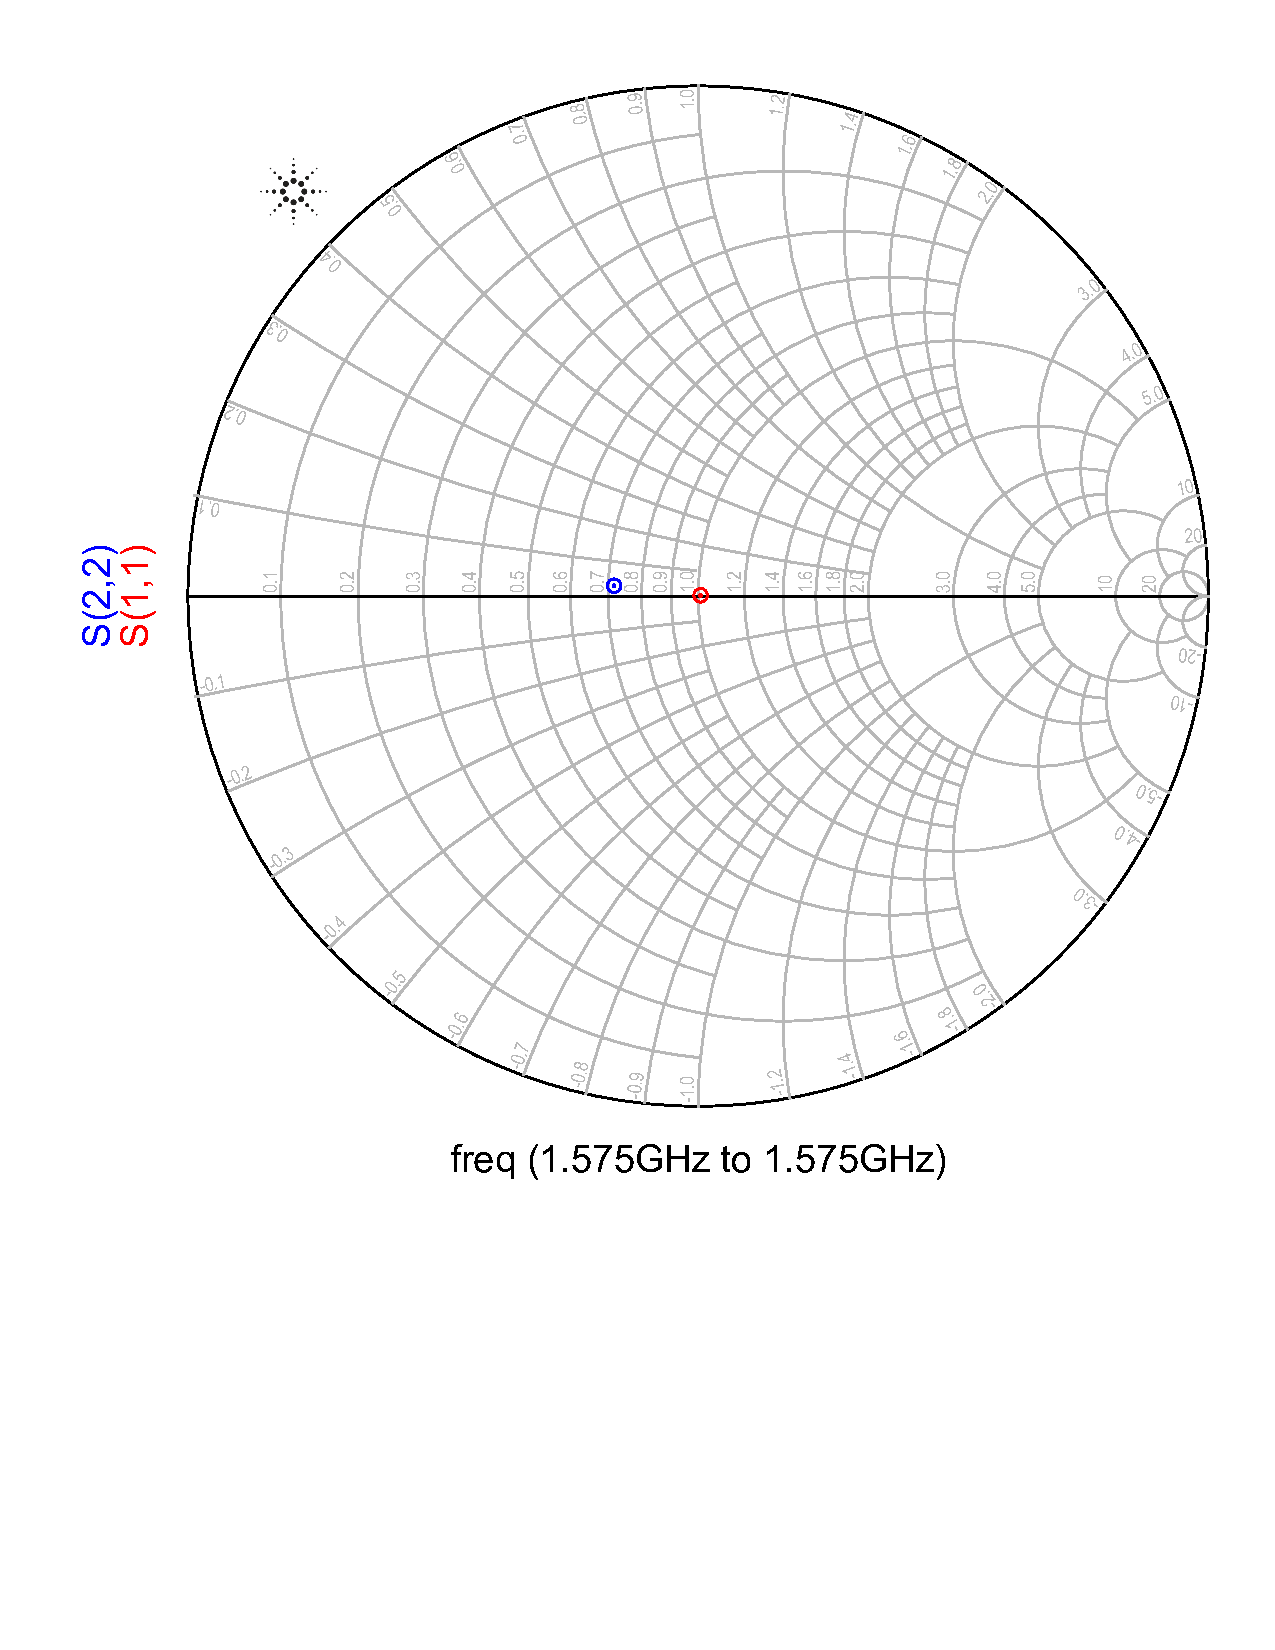
\includegraphics[width=0.5\textwidth]{fig/LNA/matching_smith.pdf}
			\caption{Smith Chart after adding matching network}
			\label{fig:lna_matching_smith}
			\end{figure}

		\subsubsection{Gain and Noise Linearity}

			To obtain the 1dB Compression Point large signal S-parameters need to be simulated. The difference between the simulated gain characteristic and the ideal (linear) gain characteristic is plotted as a function of the input power in Figure \ref{fig:lna_1dbcp}. We see that the 1-dBCP is reached for an input power equal to $\SI{-15.5}{\dbm}$. We also know that the gain of the amplifier is $\SI{20}{\decibel}$, hence we get an output referred 1-dBCP of $\SI{4.5}{\dbm}$ which is within the specifications. To increase the linearity further, we added inductive emittor degeneration with an inductor of $\SI{100}{\pico\henry}$. This will not be a physical component, but the inductance will be present due to the vias to the ground plane. 

			\begin{figure}[H]
			\centering
				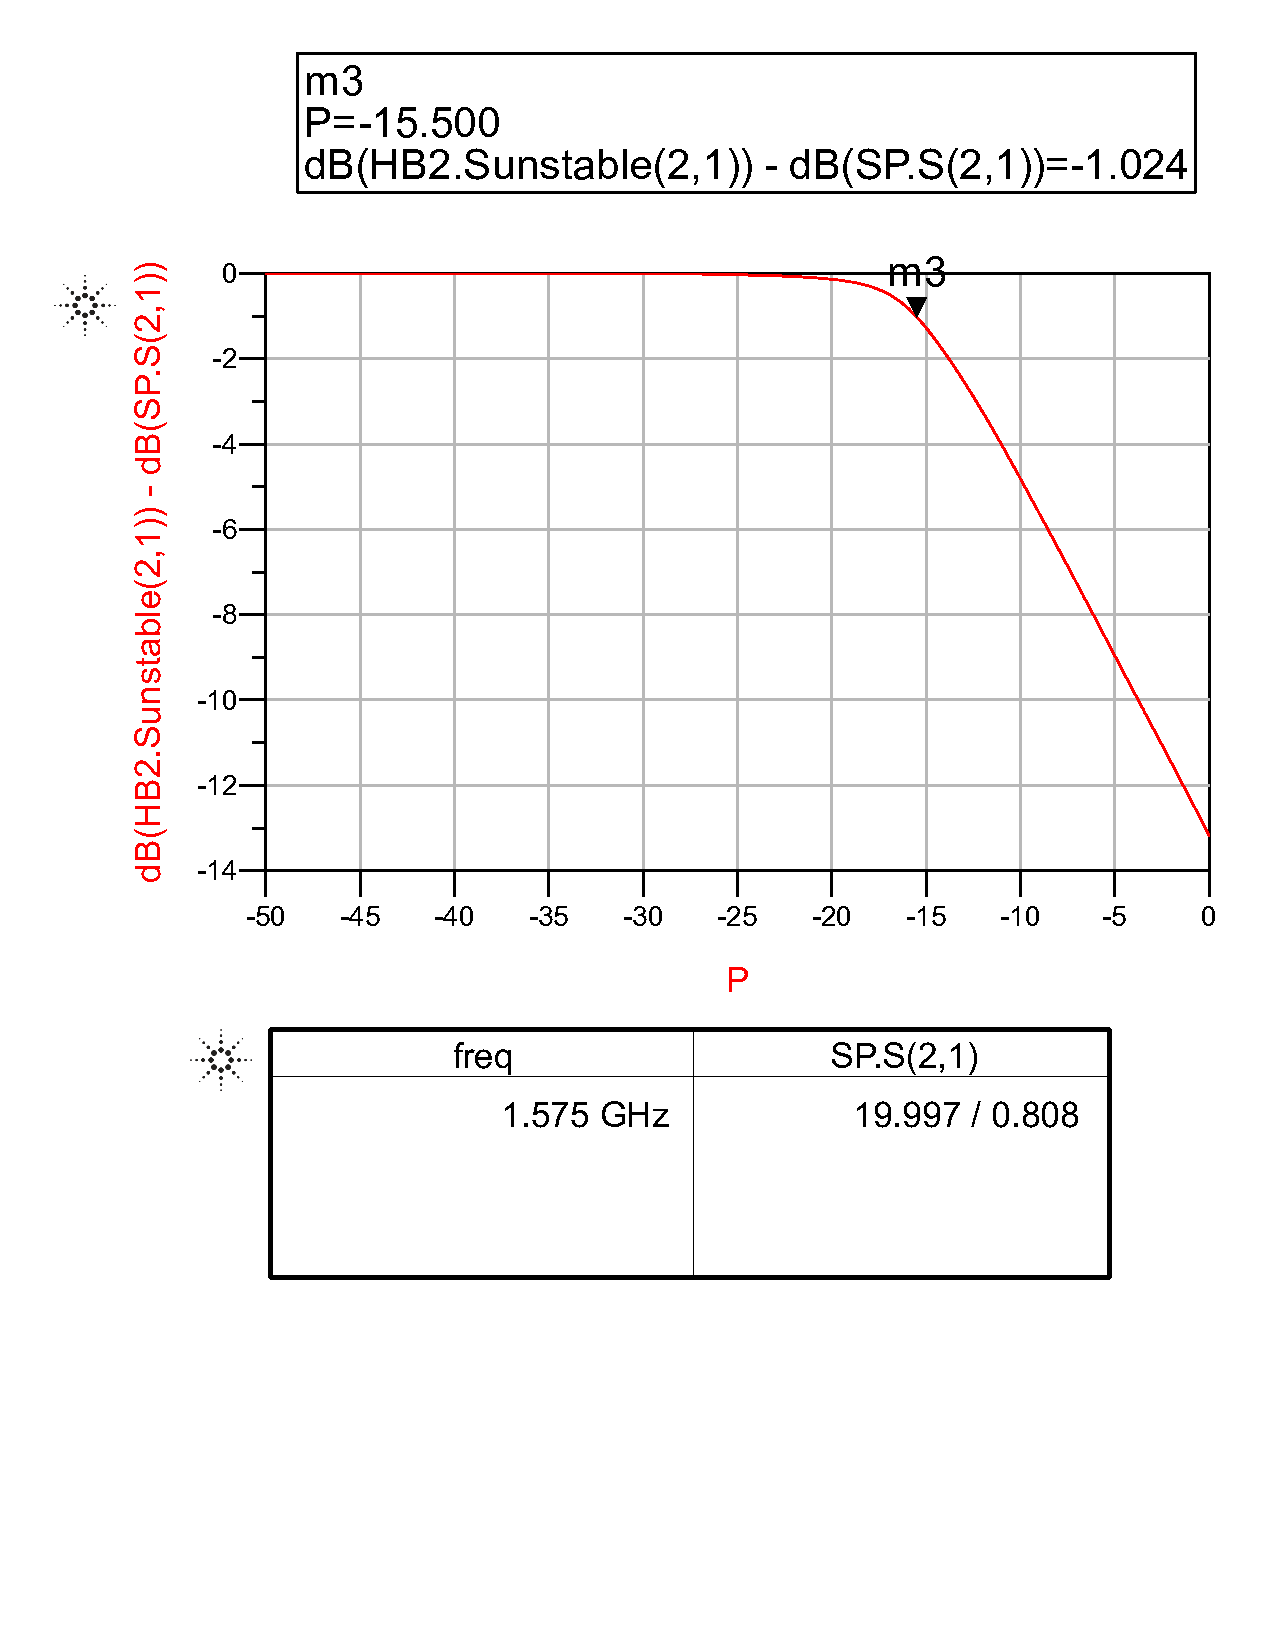
\includegraphics[width=0.5\textwidth]{fig/LNA/compression_point.pdf}
			\caption{Simulated 1 dB Compression Point}
			\label{fig:lna_1dbcp}
			\end{figure}

		\subsubsection{Figure of merit}
			We want the LNA to be as linear as possible, but the DC power consumption needs to be kept as low as possible. That's why we will use the ratio $\frac{OIP3}{P_{DC}}$ as a figure of merit (FOM), with $OIP3$ the Output Referred Third Order Intercept Point and $P_{DC}$ the DC power consumption. The higher the FOM, the higher the linearity of the amplifier and the lower the power consumption. \\

			To calculate OIP3 we perfom a Harmonic Balance simulation in ADS, i.e. we send two tones into the circuit and observe the third order mixing products. Figure \ref{fig:lna_fom} shows these third order products and their output referred intercept point in the table below the figure. 
			
			\begin{figure}[H]
				\centering
				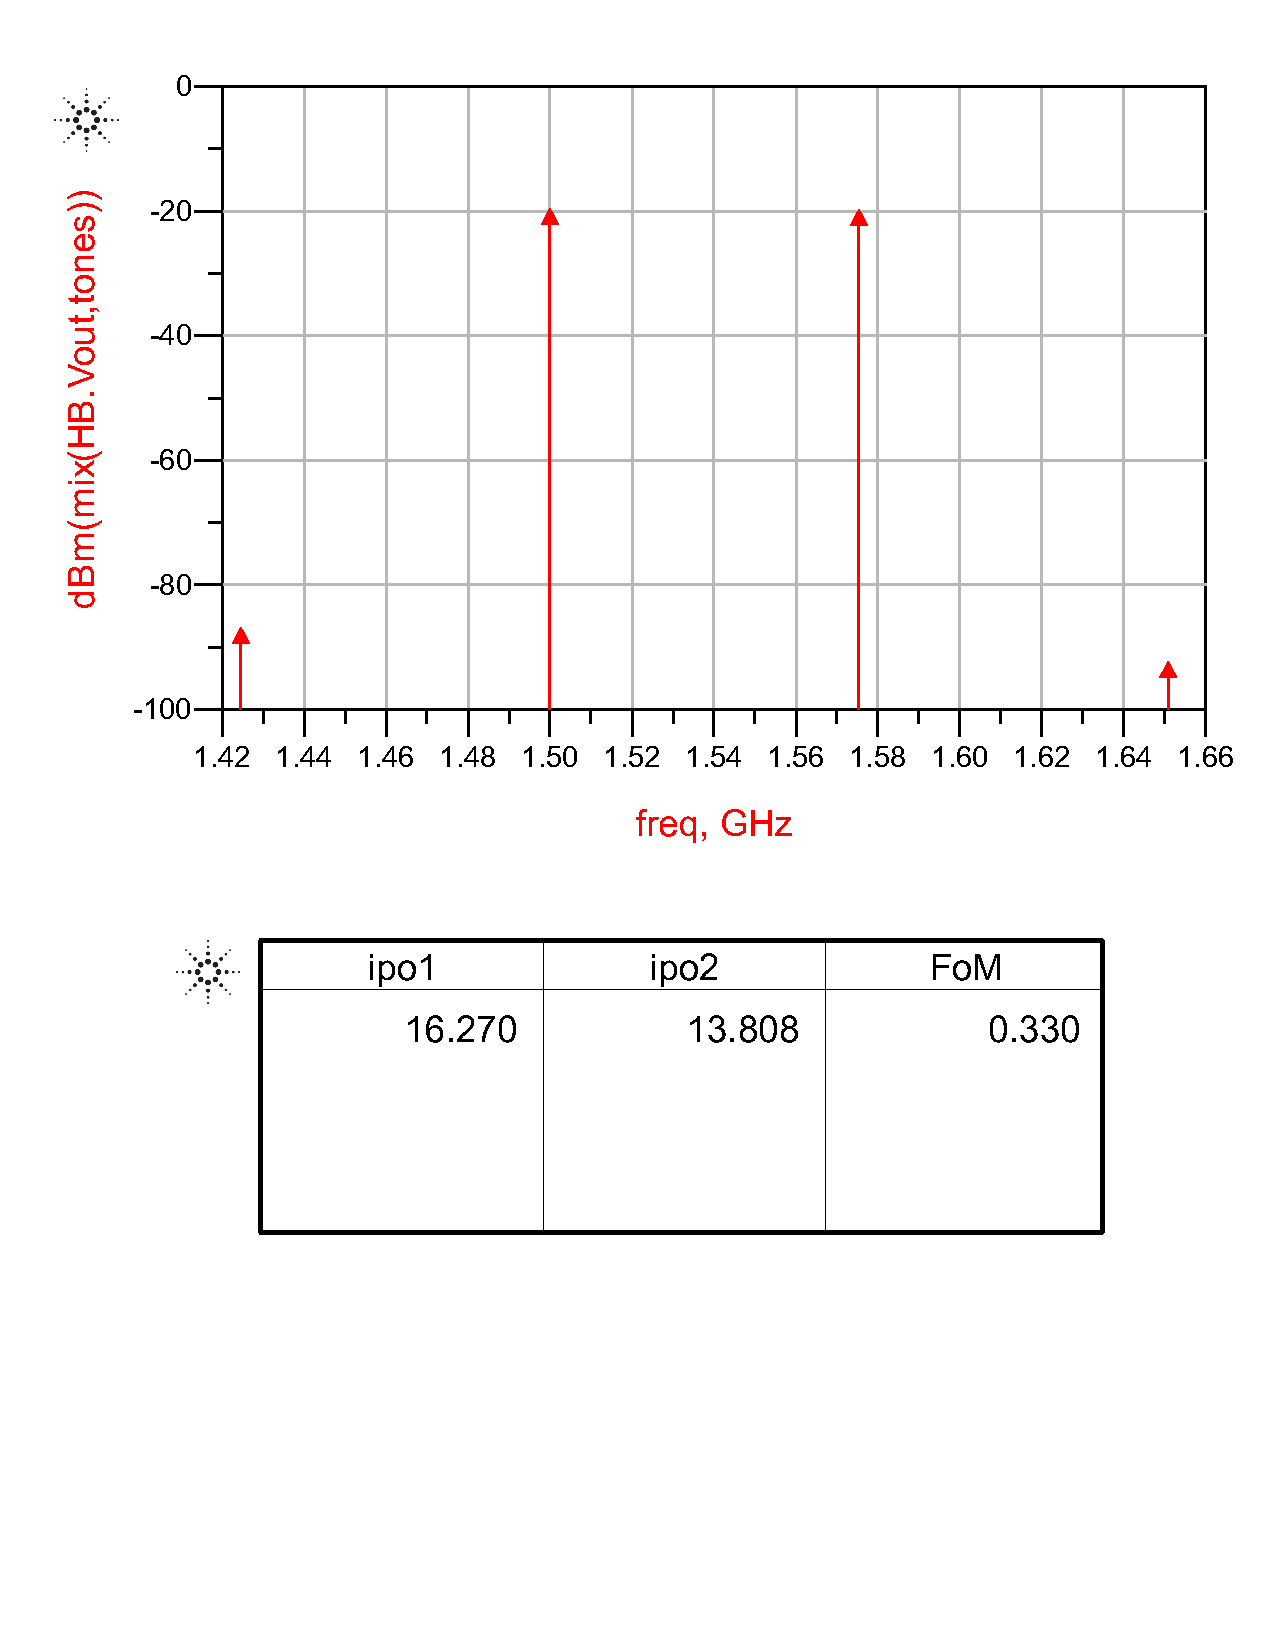
\includegraphics[width=0.5\textwidth]{fig/LNA/fom.pdf}
				\caption{Figure of merit}
				\label{fig:lna_fom}
			\end{figure}

		\subsubsection{Summary}
			Table \ref{tab:lna_summ} gives an overview of the simulated design parameters compared with the specifications. It can be seen that in this stage of the design all specifications are still met.  

			\begin{table}[H]
			\centering
			\begin{tabular}{|l|r|r|}
				\hline
				 & \textbf{Realized} & \textbf{Specs} \\
				\hline
				\textbf{SS Gain} & 20 dB & $>$ 16 dB \\
				\hline
				\textbf{NF} & 1.196 dB & $\leq$ 1.5 dB \\
				\hline
				\textbf{Output ref. 1dBCP} & 4.5 dBm & $>$ 3 dBm \\
				\hline
				\textbf{FOM} & 0.33 & n/a \\
				\hline
			\end{tabular}
			\caption{Summarizing achieved specs}
			\label{tab:lna_summ}
			\end{table}

		
	\subsection{Filter}
  To remove as much noise and unwanted signals as possible, a filter will be placed in front of the LNA. This filter should of course pass the desired GPS signal and block the nearby GSM-1800 frequencies, of which the closest is $\SI{1710}{\mega\hertz}$.
  \subsubsection{Prototype}
  In order to design the filter, we start from a $2^{nd}$ order elliptic prototype. This filter consists of one capacitor and one inductor with an equal nominal value of $\sqrt{2}$.  It is matched to $\SI{1}{\ohm}$ ports and has a lowpass characteristic with a cut-off frequency of $\SI{1}{\hertz}$.
  The prototype is transformed into a bandpass filter using following transformations\cite{coupled_lines}:
  \begin{eqnarray*}
    C_p &=& \frac{C}{Z_0 \omega_0 \Delta f}\\
    L_p &=& \frac{Z_0 \Delta f}{C \omega_0}\\
    L_s &=& \frac{L Z_0}{\omega_0 \Delta f}\\
    C_s &=& \frac{\Delta f}{L Z_0 \omega_0}
  \end{eqnarray*}
  Here $\Delta f$ is given by $\frac{BW}{f_0}$. We set the bandwidth to $\SI{30}{\mega\hertz}$ as we found out that in later iterations the bandwidth has the tendency to decrease.
  \begin{figure}[H]
    \centering
    \begin{subfigure}{0.5\textwidth}
      \centering
      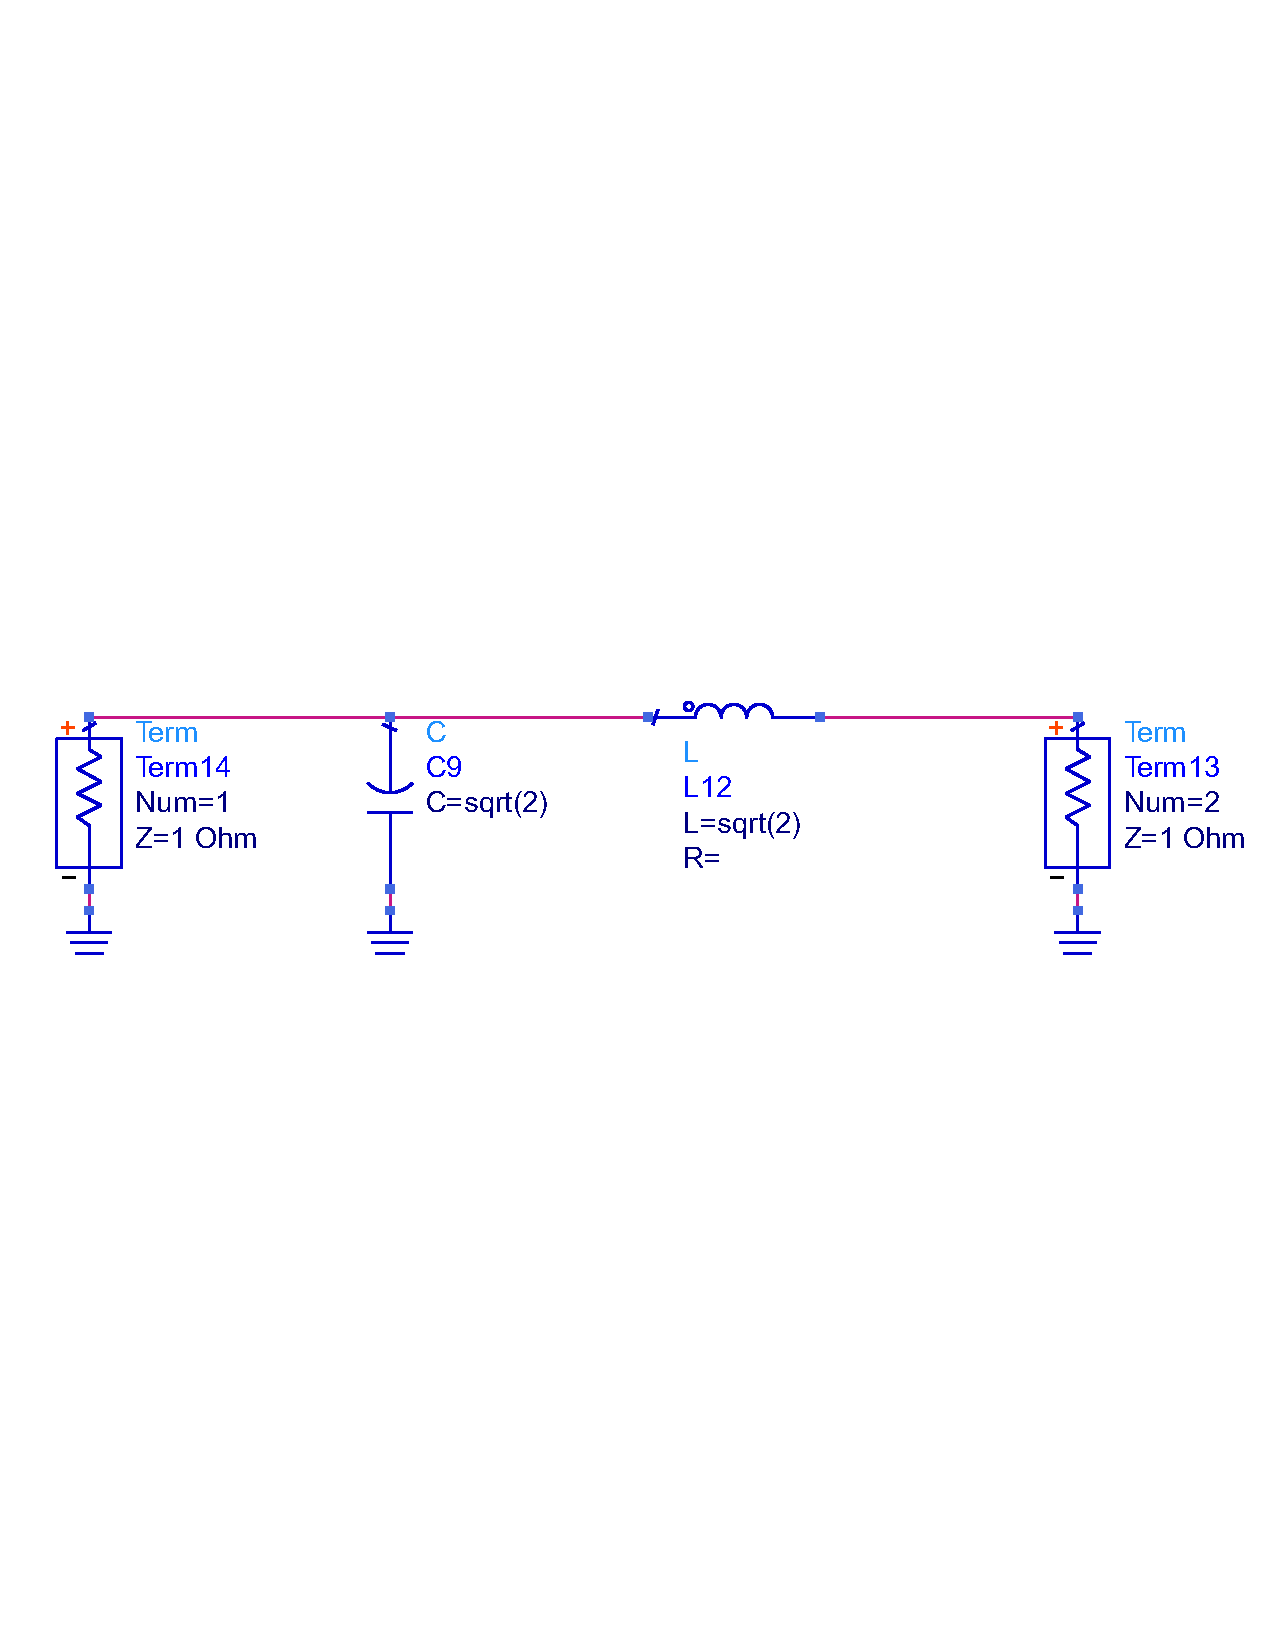
\includegraphics[width=\textwidth]{fig/Filter/2nd_order/proto_1.pdf}
      \caption{Capacitor - Inductor}
      \label{fig:proto_capin}
    \end{subfigure}%
    \begin{subfigure}{0.5\textwidth}
      \centering
      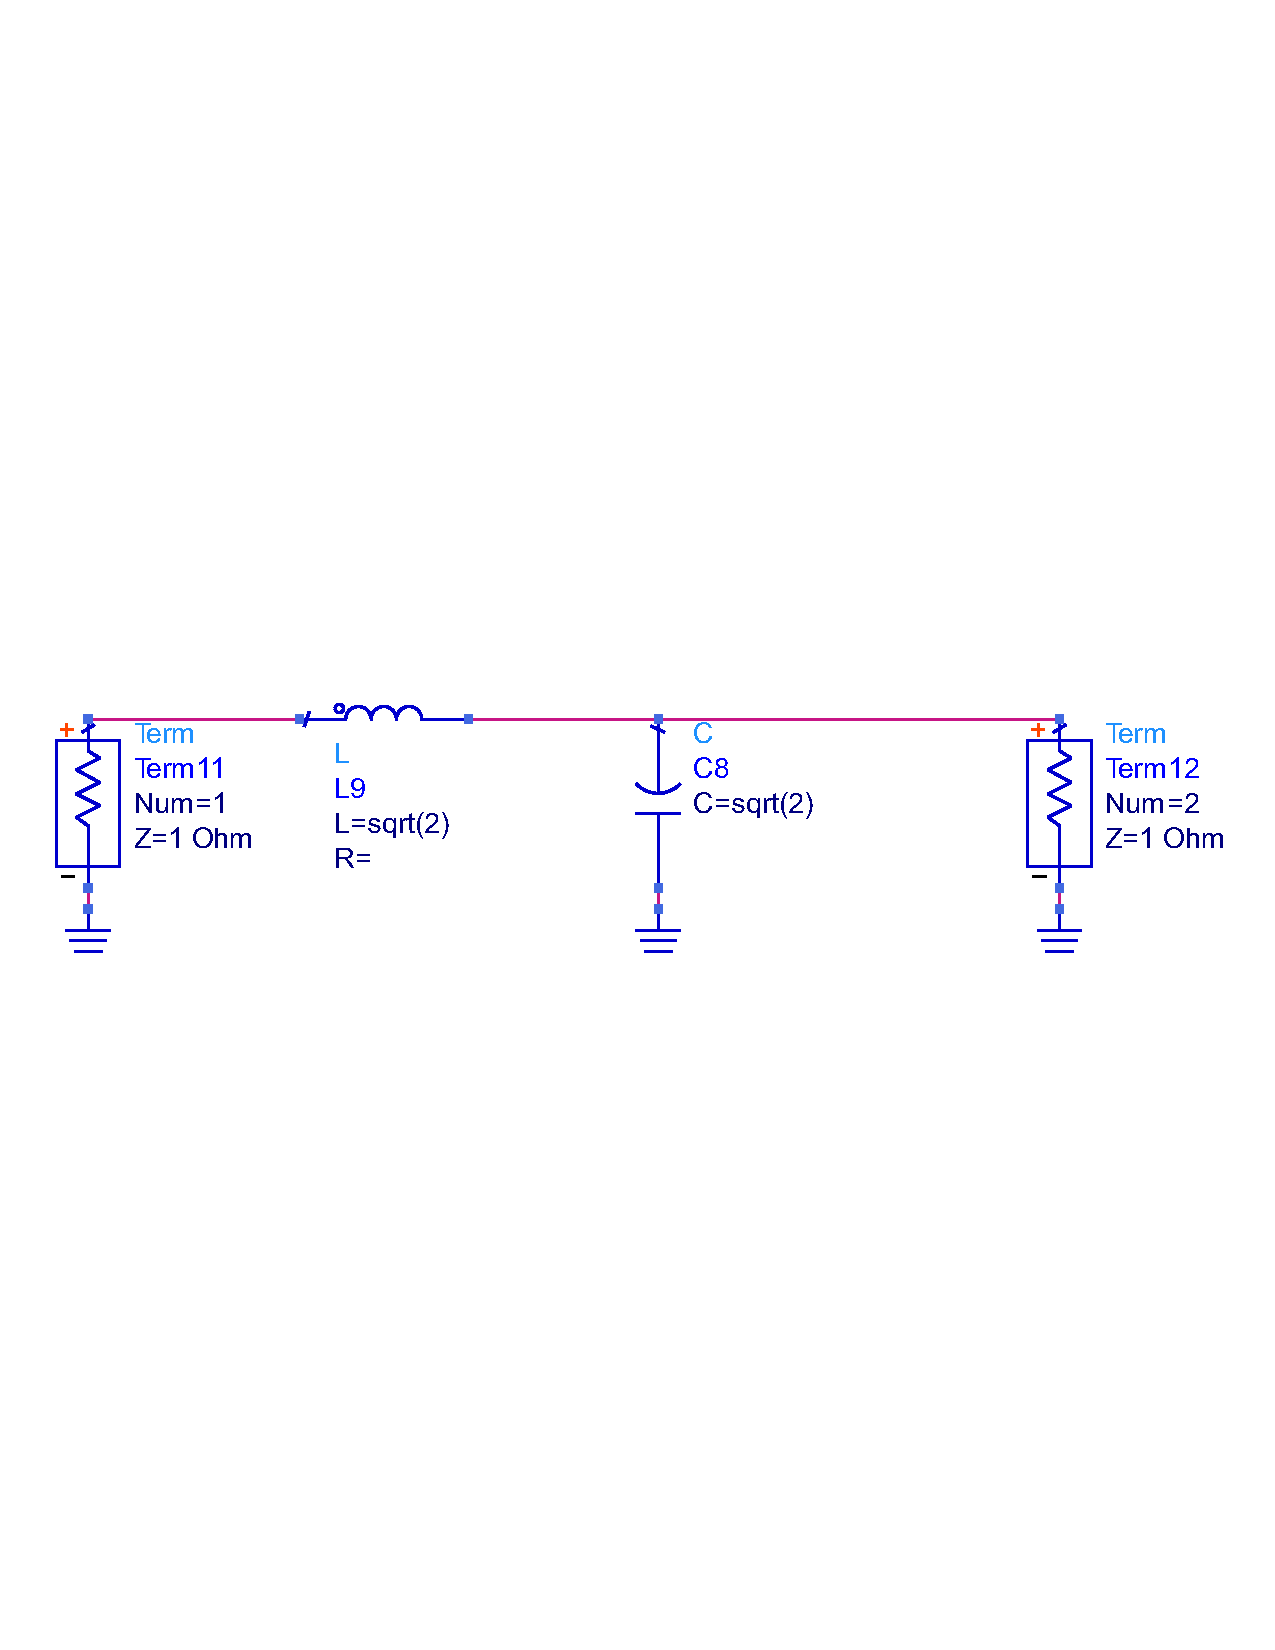
\includegraphics[width=\textwidth]{fig/Filter/2nd_order/proto_2.pdf}
      \caption{Inductor - Capacitor}
      \label{fig:proto_incap}
    \end{subfigure}
    \caption{Prototype Filters}
    \label{fig:proto}
  \end{figure}

  For this design we followed the shunt-C transformation where via the use of quarter-wavelength transformers, the parallel resonators are replaced by their series equivalent. To ease calculations, we start from two prototypes (\autoref{fig:proto}) and combine these later on.

  Using the transformations above, the schematics in \autoref{fig:filter_transform} are found.

  \begin{figure}[H]
    \centering
    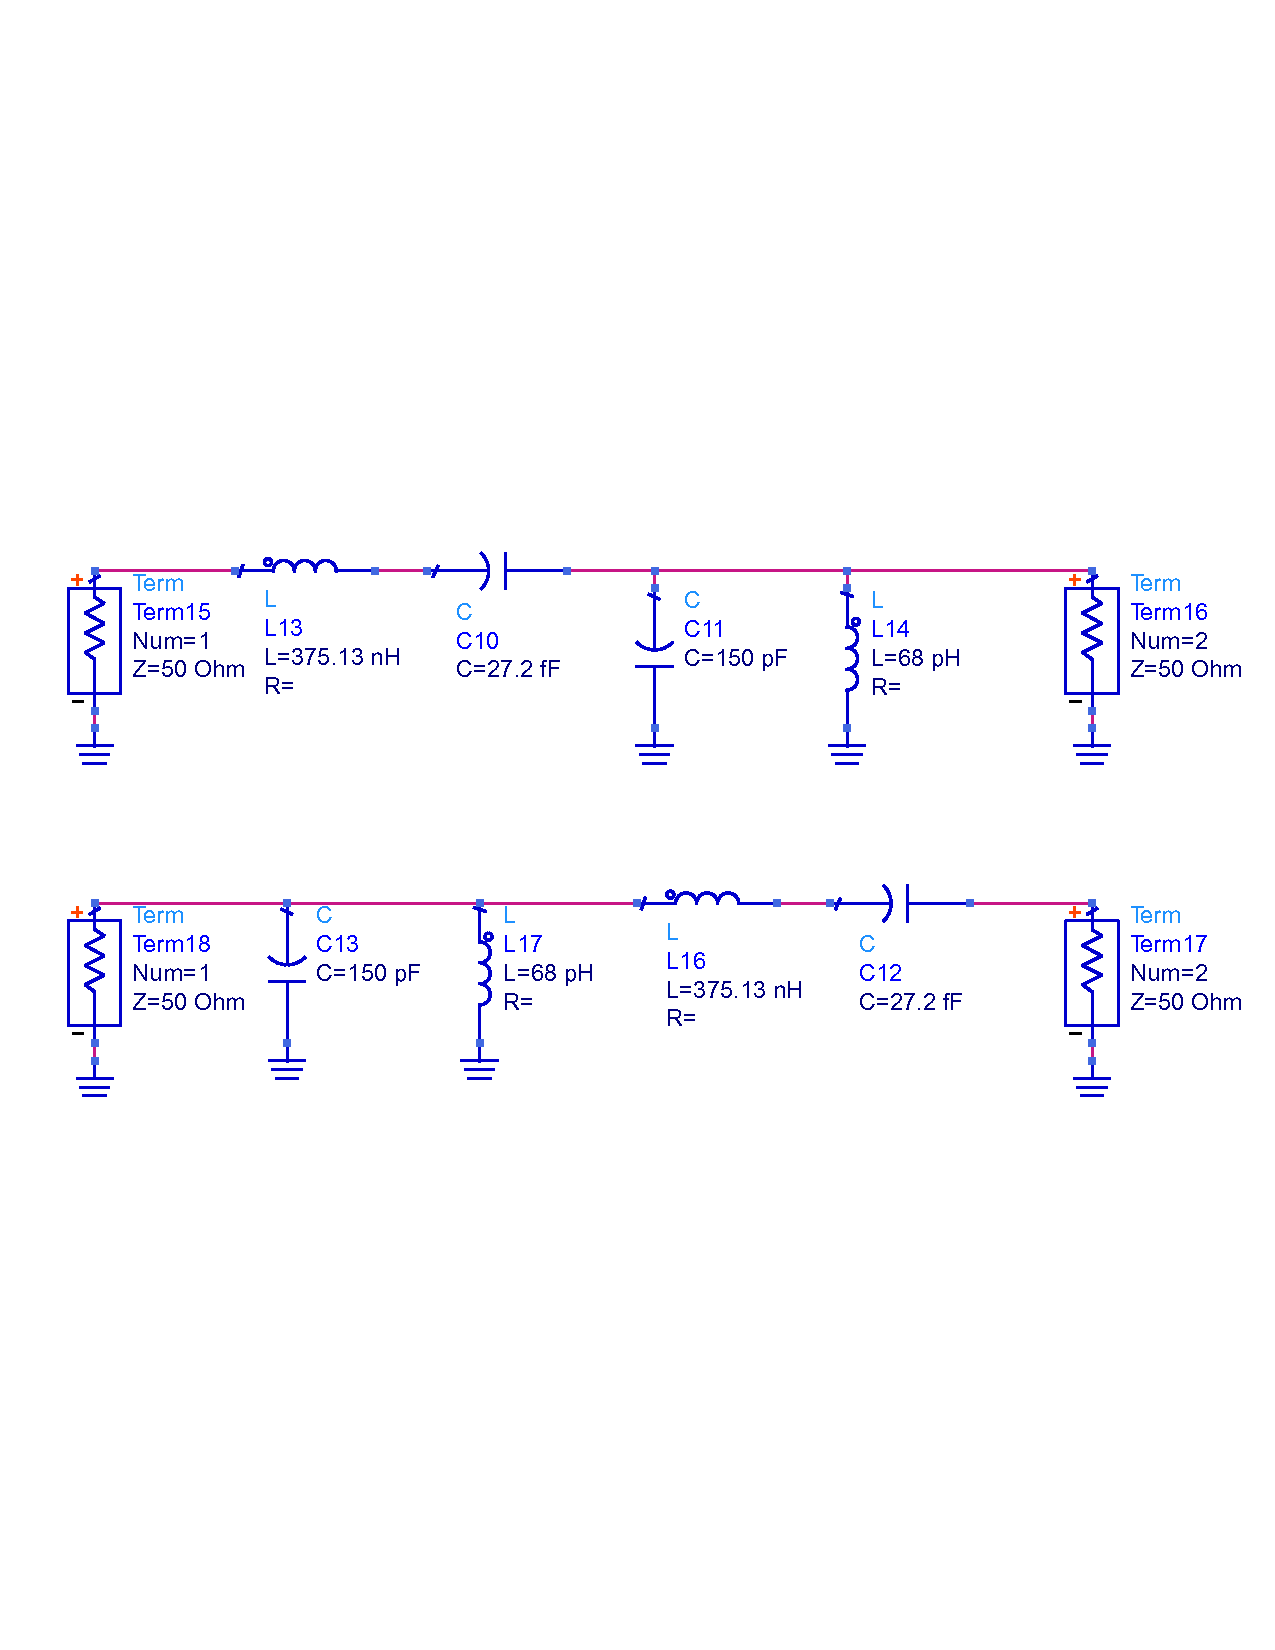
\includegraphics[width=\textwidth]{fig/Filter/2nd_order/bandpass_discrete.pdf}
    \caption{Transformation to bandpass filter}
    \label{fig:filter_transform}
  \end{figure}

  \subsubsection{Transmission line transformation}
  Both filters in \autoref{fig:filter_transform} are combined in \autoref{fig:filter_series_res} using quarter-wavelength transformers. 
  The series resonators can be replaced by transmission line sections in a narrowband approximation (\autoref{fig:filter_transmission_line}).

  \begin{figure}[H]
    \centering
    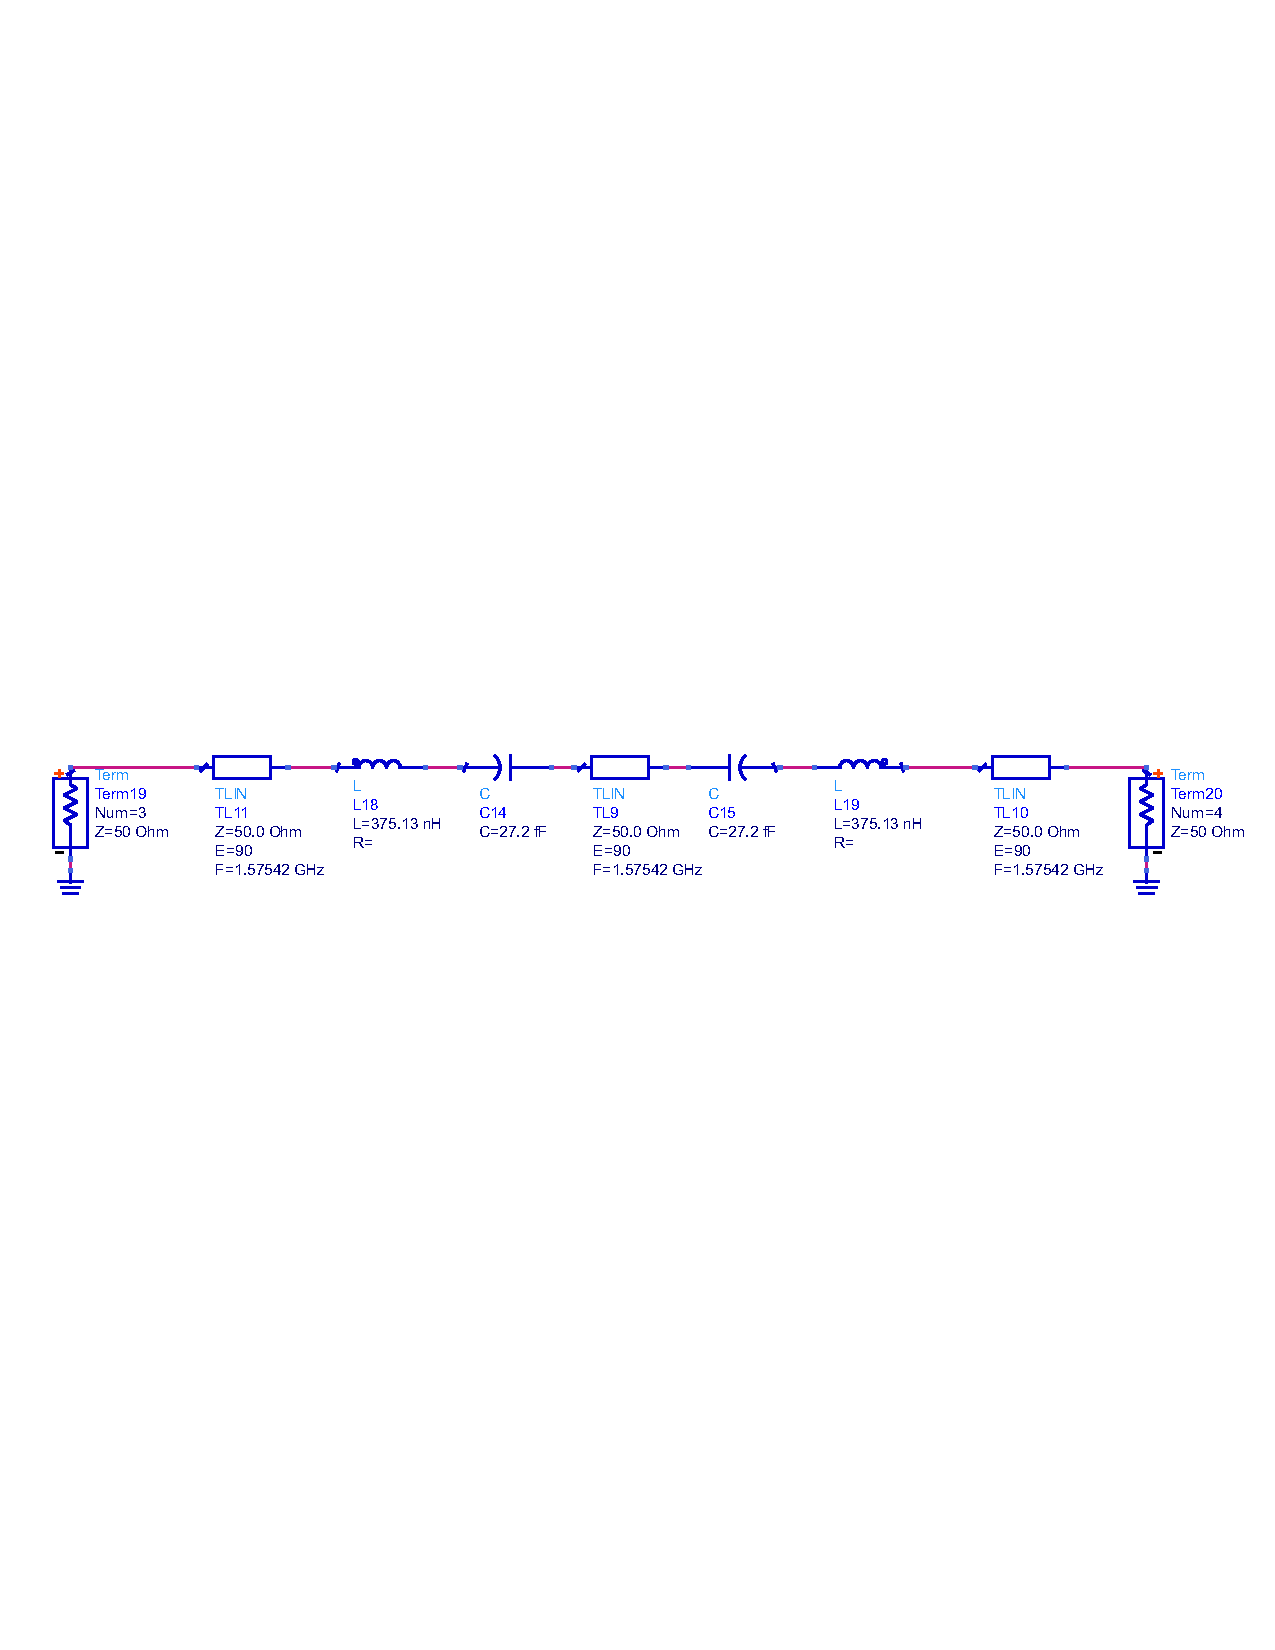
\includegraphics[width=\textwidth]{fig/Filter/2nd_order/bandpass_discrete_only_series_res.pdf}
    \caption{Substitution with Quarter-wavelength transformers}
    \label{fig:filter_series_res}
  \end{figure}

  \begin{figure}[H]
    \centering
    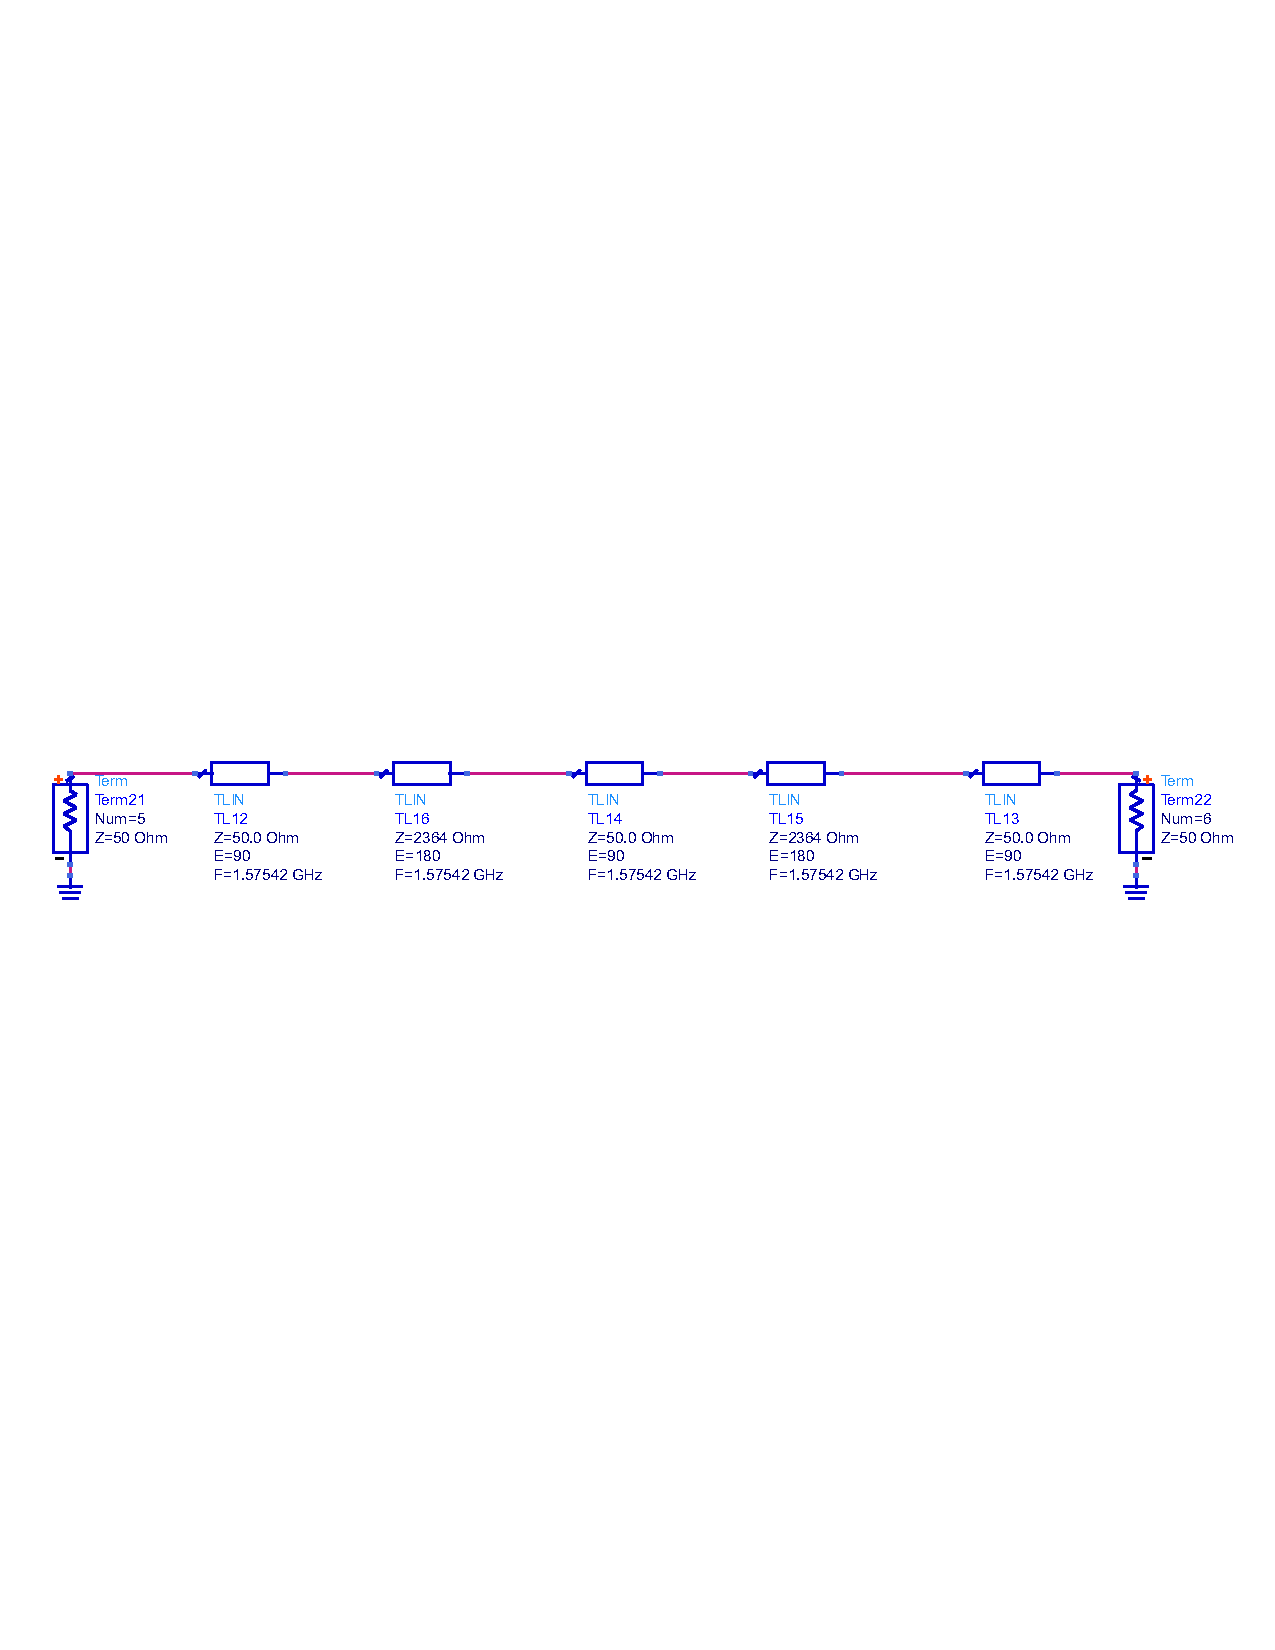
\includegraphics[width=\textwidth]{fig/Filter/2nd_order/bandpass_series_res_to_TL.pdf}
    \caption{Transmission line only implementation}
    \label{fig:filter_transmission_line}
  \end{figure}

  The S-parameters for the schematics from Figures \ref{fig:filter_series_res} and \ref{fig:filter_transmission_line} are shown in Figure \ref{fig:filter_spar_TL}. Replacing the discrete series resonators with transmission lines has no significant effect on the S-parameters, because the bandwidth was already determined by the quarter wavelength transformers. The realized filter is within the specifications, i.e. no attenuation in the passband (ideal components are used) and more than $\SI{20}{\decibel}$ attenuation in the GSM1800-band.  

  \begin{figure}[H]
  \centering
  	\begin{subfigure}{0.7\textwidth}
  	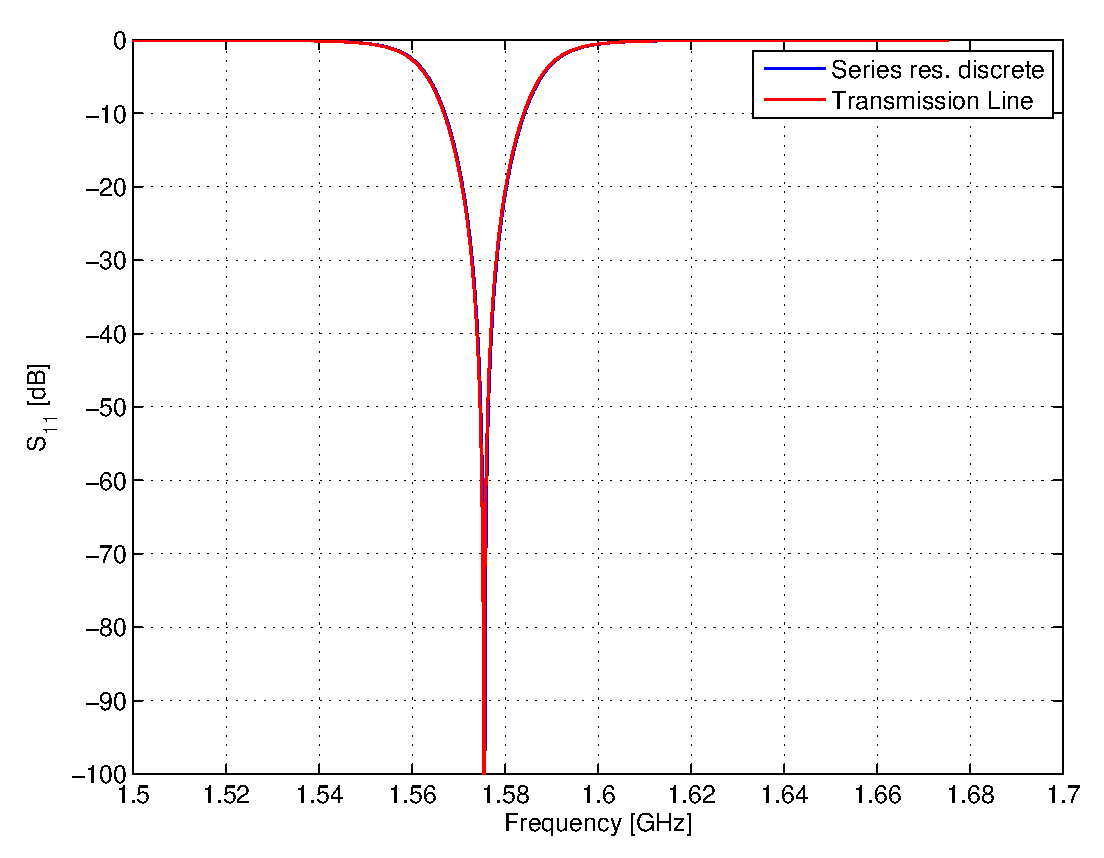
\includegraphics[width=\textwidth]{fig/Filter/2nd_order/plots/S11_TL.eps}
  	\end{subfigure}
  	\begin{subfigure}{0.7\textwidth}
  	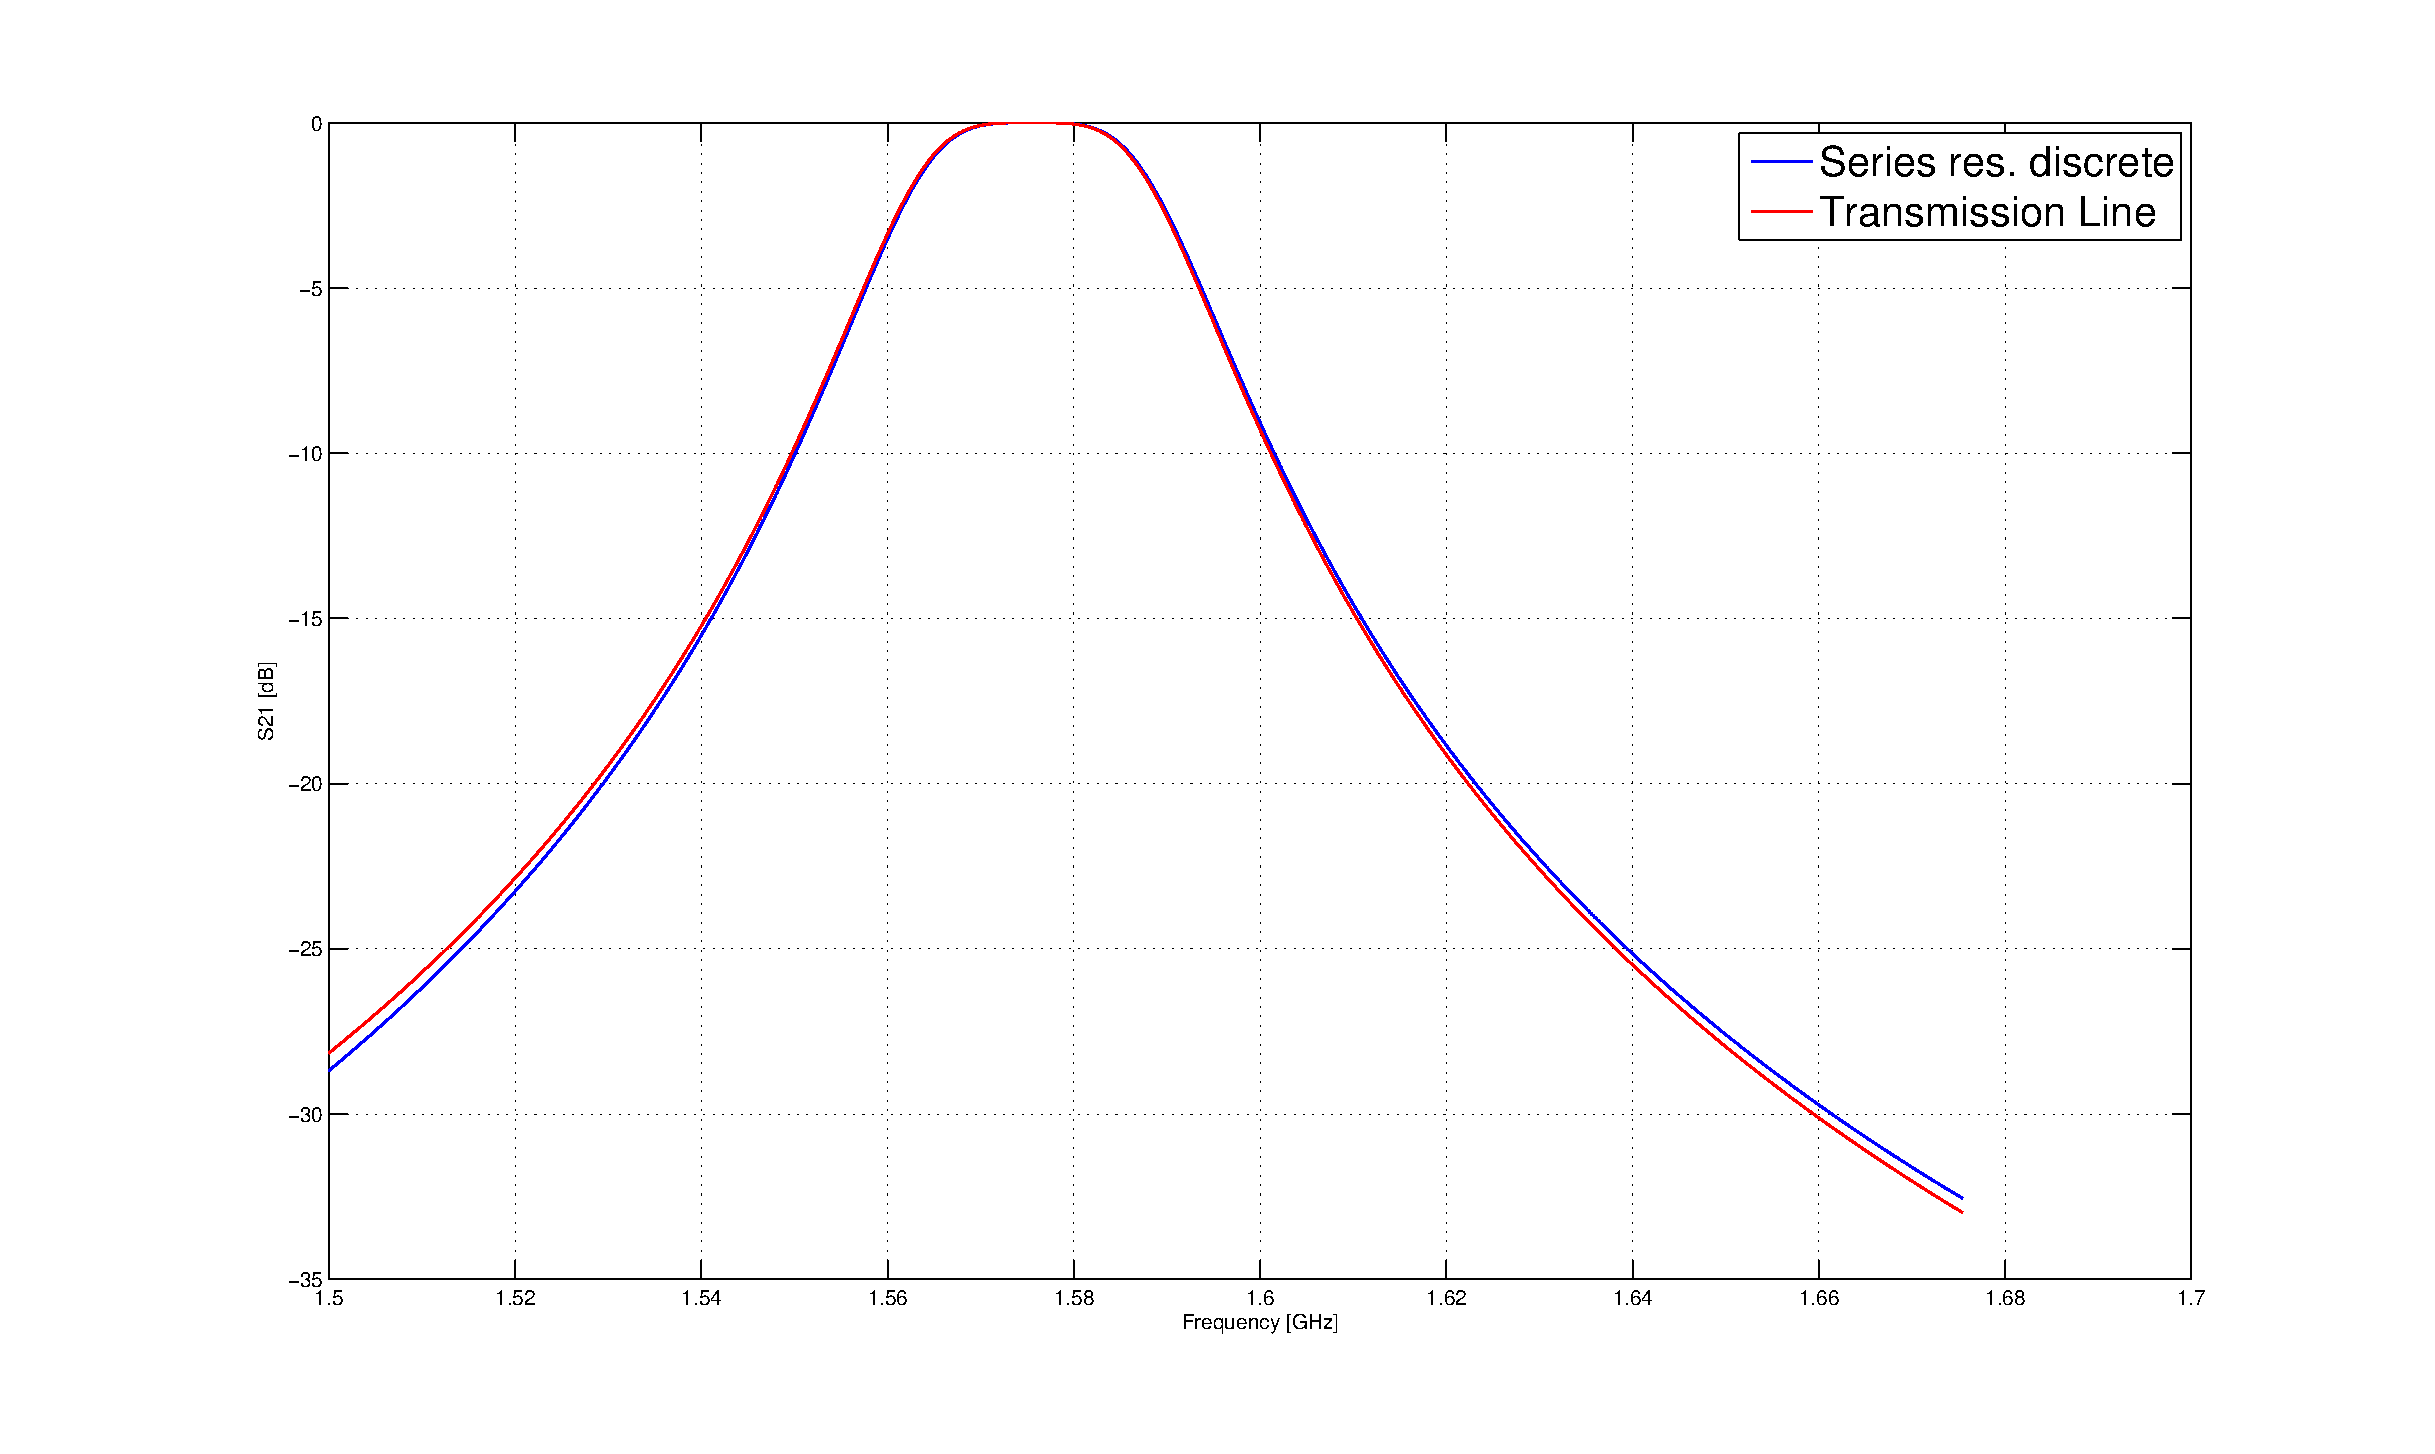
\includegraphics[width=\textwidth]{fig/Filter/2nd_order/plots/S21_TL.eps}
  	\end{subfigure}
  	\caption{S-parameters for TL only implementation}
  	\label{fig:filter_spar_TL}
  \end{figure}

  These transmission lines have a characteristic impedance derived from the values of the capacitor and inductor in the resonator via following relation\cite{coupled_lines}: 
  \begin{eqnarray*}
    Z_0 &=& \frac{2 \omega_{res} L_s}{\pi},\\
    \omega_{res} &=& \frac{1}{\sqrt{C_s L_s}}
  \end{eqnarray*}

  The solution of these equations yields an impossibly high impedance and we rescale these impedances to $\SI{50}{\ohm}$. To this end the $\SI{50}{\ohm}$ sections of $\SI{90}{\degree}$ can be seen as quarter-wavelength transformers, hence it holds that

  \begin{align}
  	Z_{in} &= \frac{Z_0^2}{Z_L}
  \label{eq:quarter_TL}
  \end{align}

  with $Z_0$ the impedance of the transformer, $Z_L$ the load impedance and $Z_{in}$ the input impedance\cite{pozar}. In case of Figure \ref{fig:filter_transmission_line} we want to rescale the $\SI{2364}{\ohm}$ TLs of $\SI{180}{\celsius}$ to $\SI{50}{\ohm}$ to ease the transformation to coupled lines in the following step and to get rid of the impossibly realisable impedances. We want to rescale $Z_L$ with a factor $\frac{50}{2364}$, but retain the same $Z_{in}$. Taking into account (\ref{eq:quarter_TL}) $Z_0$ needs to be scaled with $\sqrt{\frac{50}{2364}}$, yielding a $Z_0$ equal to $\SI{7.27}{\ohm}$.
  To restore the balance the section $TL_{14}$ is rescaled to this $Z_0$ as well.
  The second resonator is resized in the same manner, rescaling the $Z_0$ of $TL_{14}$ yet again by $\sqrt{\frac{50}{2364}}$, resulting in an impedance of $\SI{1.06}{\ohm}$.

  \begin{figure}[H]
    \centering
    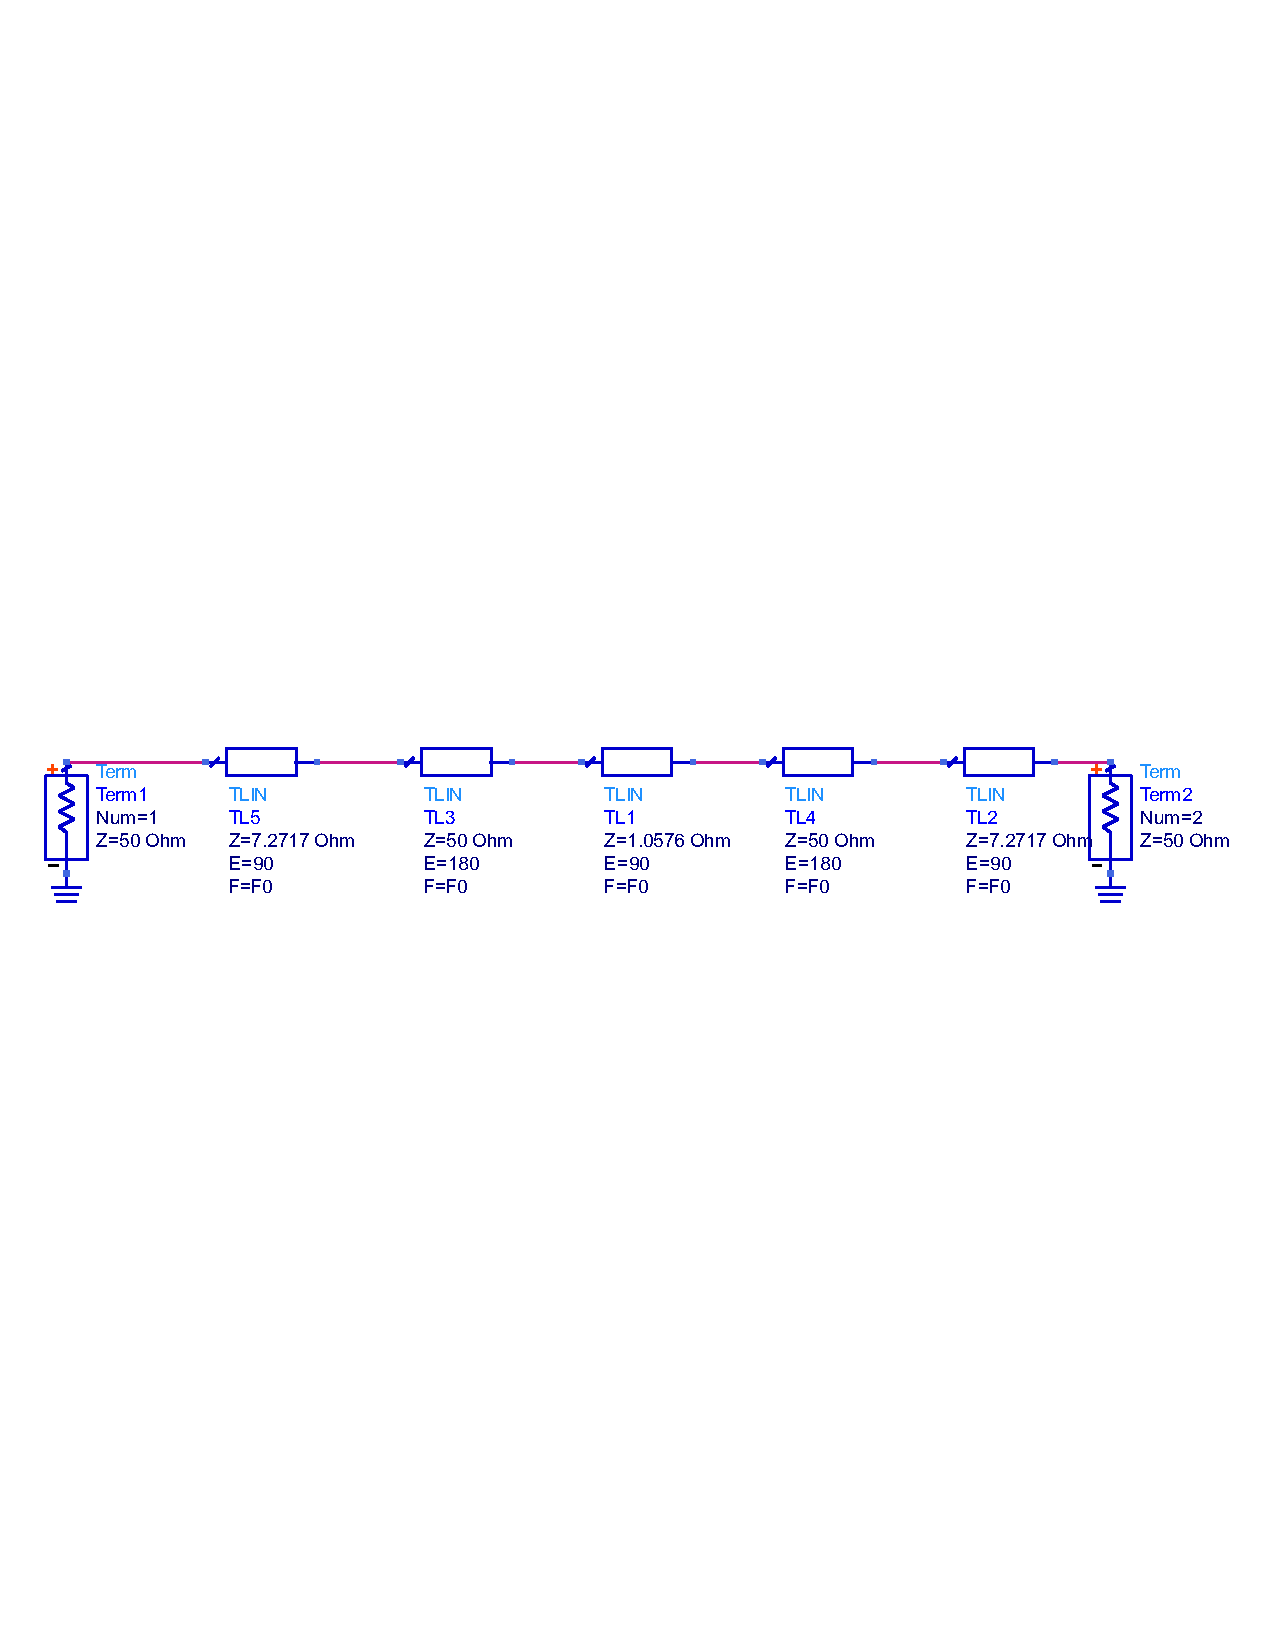
\includegraphics[width=\textwidth]{fig/Filter/2nd_order/bandpass_TL_rescaled_imp.pdf}
    \caption{Resized Transmission line segments}
    \label{fig:filter_transmission_resized}
  \end{figure}

  \subsubsection{Coupled Lines}

  	The next step is transforming to a coupled lines filter, according to the transformation shown in Figure \ref{fig:filter_CL_transform} with:
  	\begin{align}
  		\begin{cases}
  			J' = \frac{J}{Z_0 sin(\theta)} \\
  			Z_e = Z_0 (1 + J' + J'^2) \\
  			Z_o = Z_0 (1 - J' + J'^2)
  		\end{cases}
  	\end{align}

  	\begin{figure}[H]
  		\centering
  		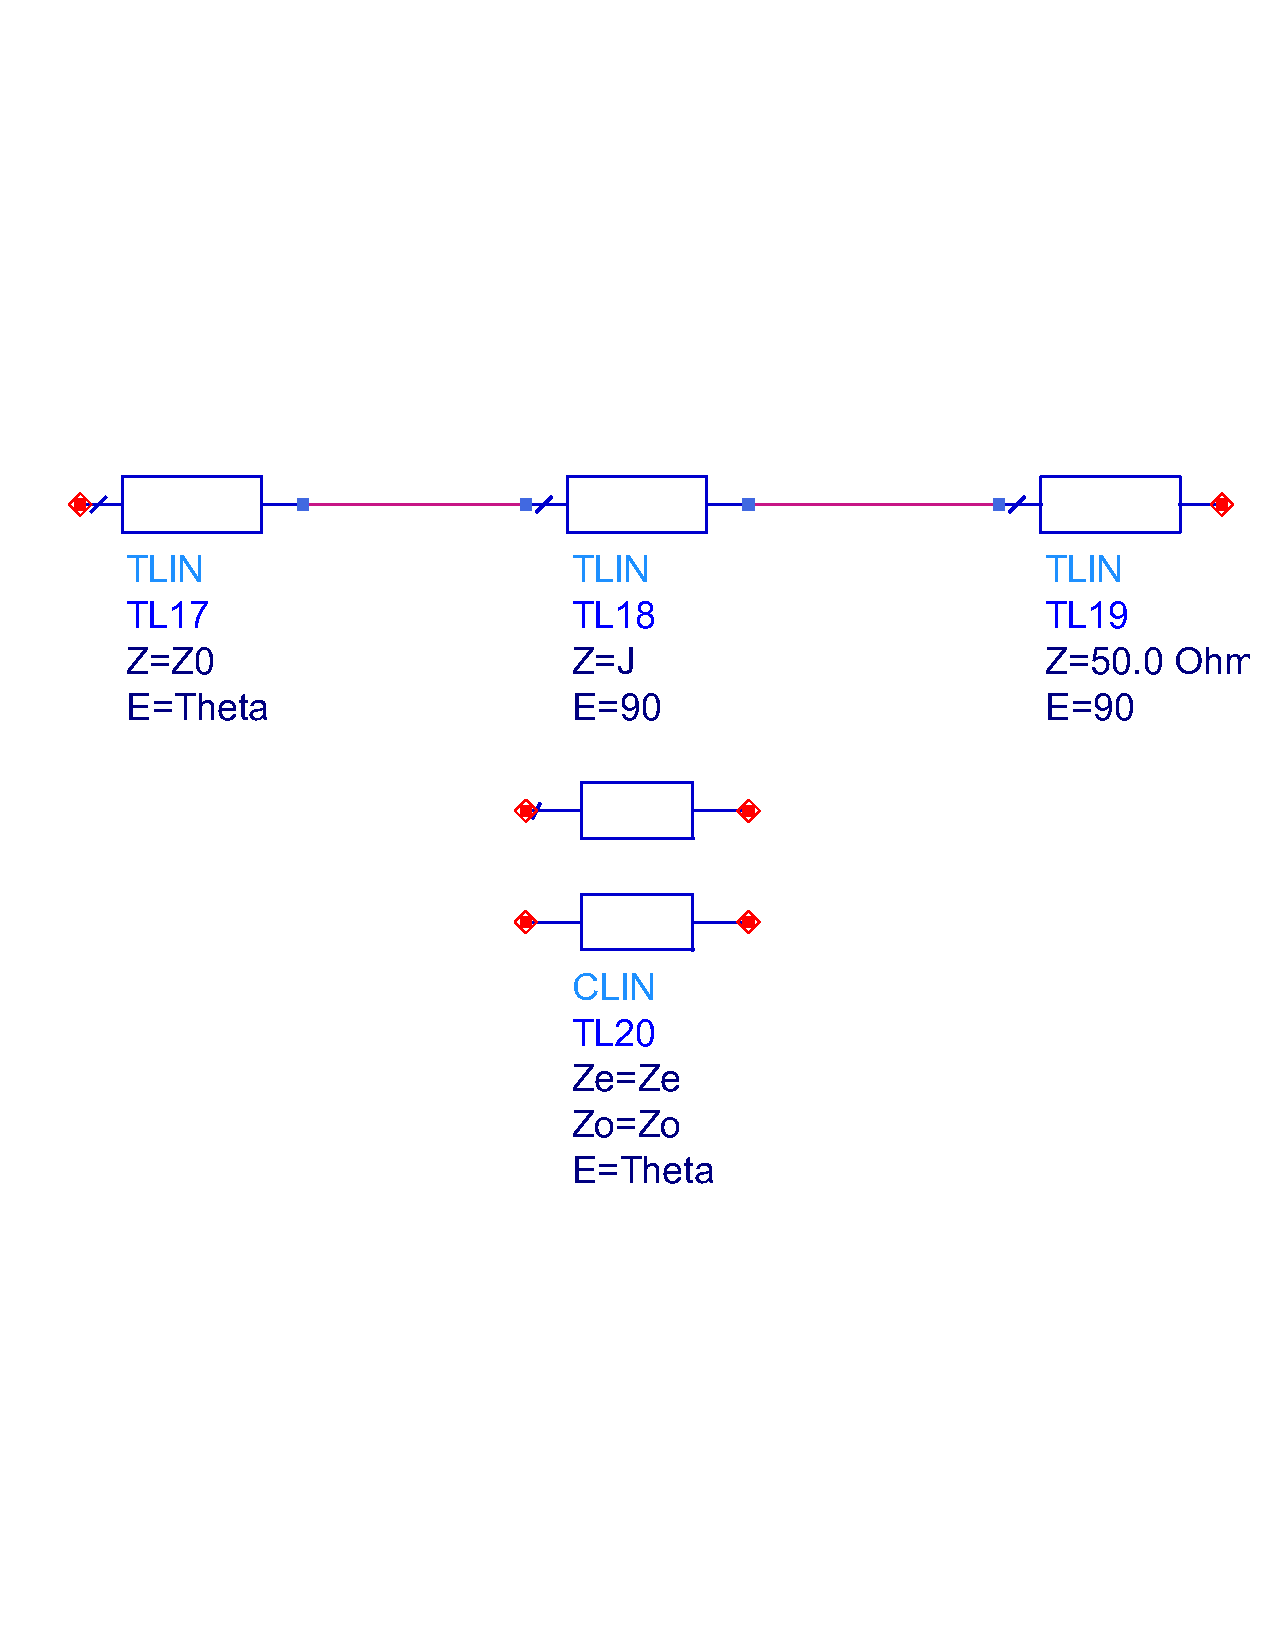
\includegraphics[width=0.5\textwidth]{fig/Filter/2nd_order/CL_transformation.pdf}
  		\caption{Transformation to coupled lines}
  		\label{fig:filter_CL_transform}
  	\end{figure} 

  	After the transformation to coupled lines, the ideal lines are substituted with microstrip lines and the substrate is added to the design. The dimensions of the coupled lines are calculated from the even and odd impedances using LineCalc. The final schematic is shown in Figure \ref{fig:filter_final_CL}. 

  	\begin{figure}[H]
  		\centering
  		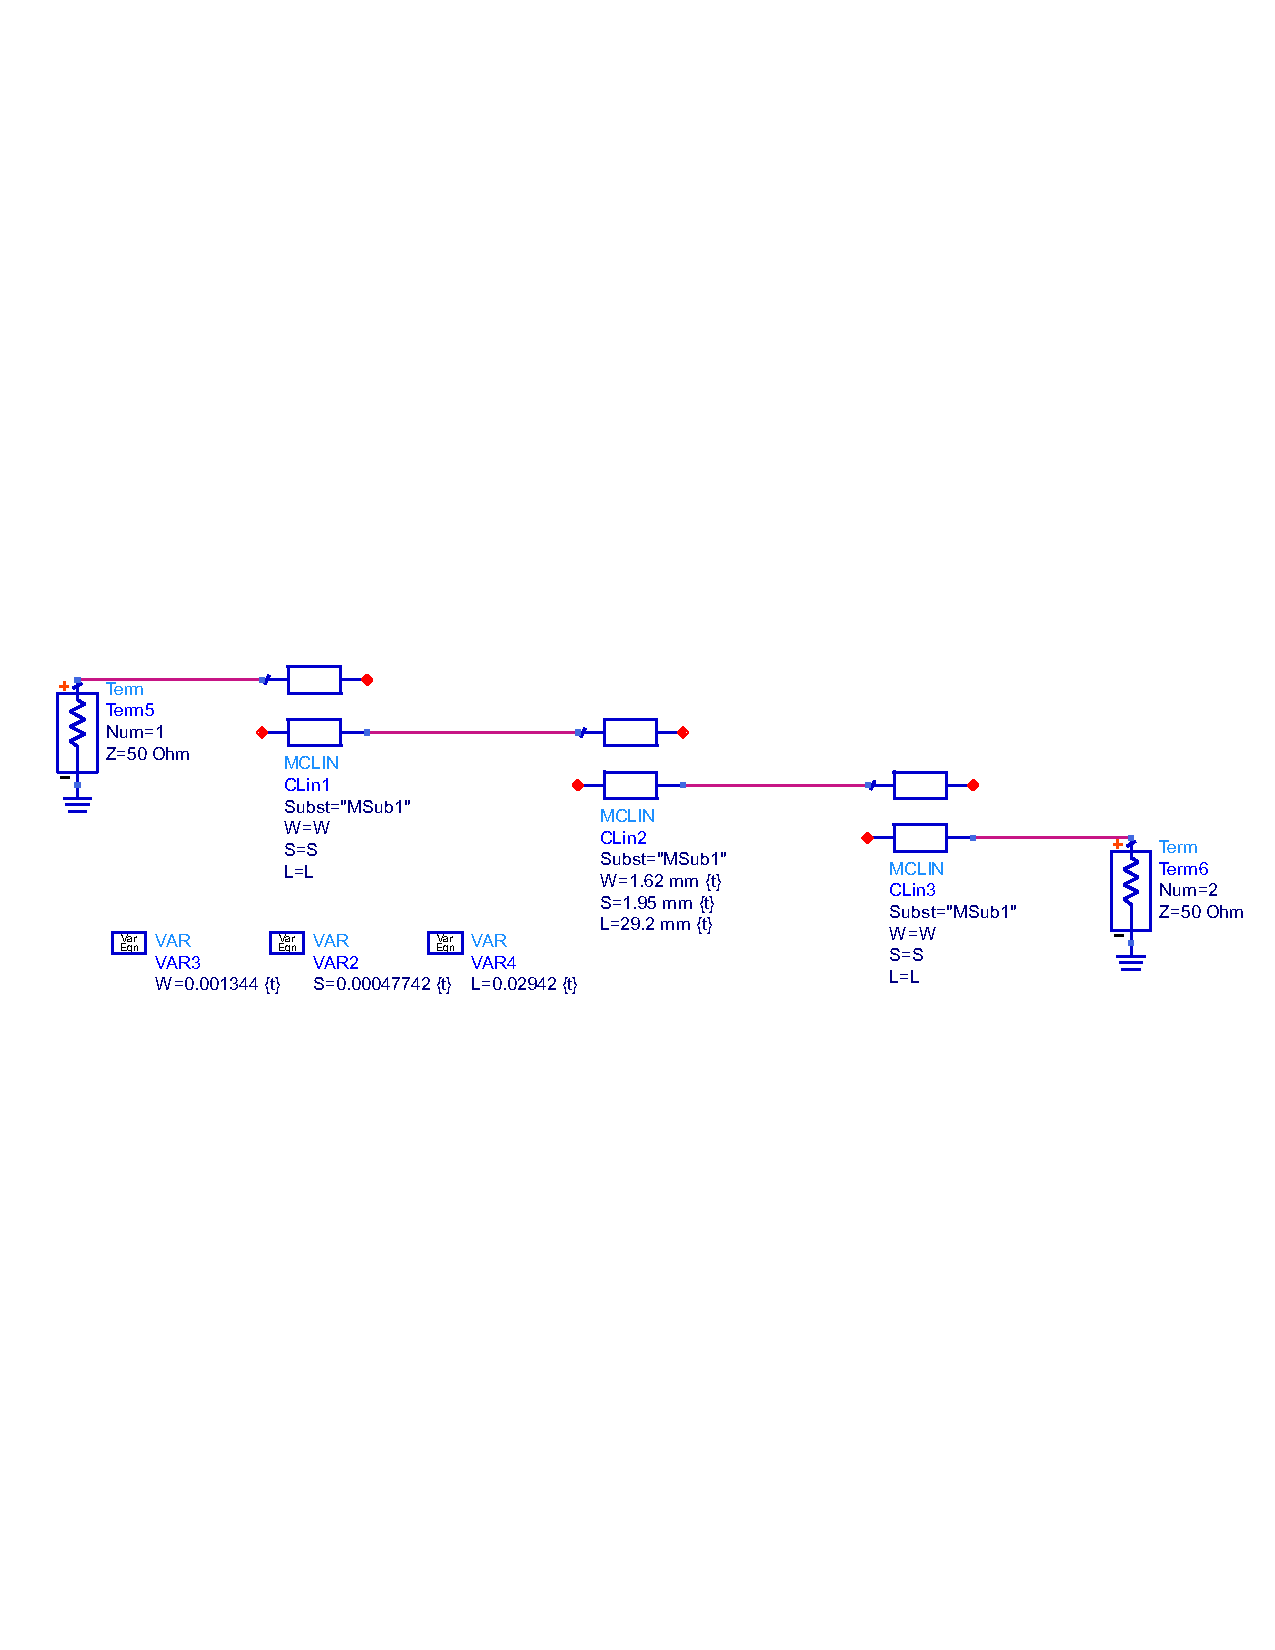
\includegraphics[width=0.9\textwidth]{fig/Filter/2nd_order/bandpass_subst_CL.pdf}
  		\caption{Coupled lines filter}
  		\label{fig:filter_final_CL}
  	\end{figure} 

  	The S-parameters for the coupled lines with added substrate are shown in Figure \ref{fig:filter_spar_subst_CL}. The most important change is the attenuation added in the passband due to substrate losses, as seen in Figure \ref{fig:filter_spar_subst_CL}, but with $\SI{1.3}{\decibel}$ still within the specification of $\SI{2}{\decibel}$. The bandwidth of the filter is approximately $\SI{50}{\mega\hertz}$.

  \begin{figure}[H]
  		\centering
  	\begin{subfigure}{0.8\textwidth}
  	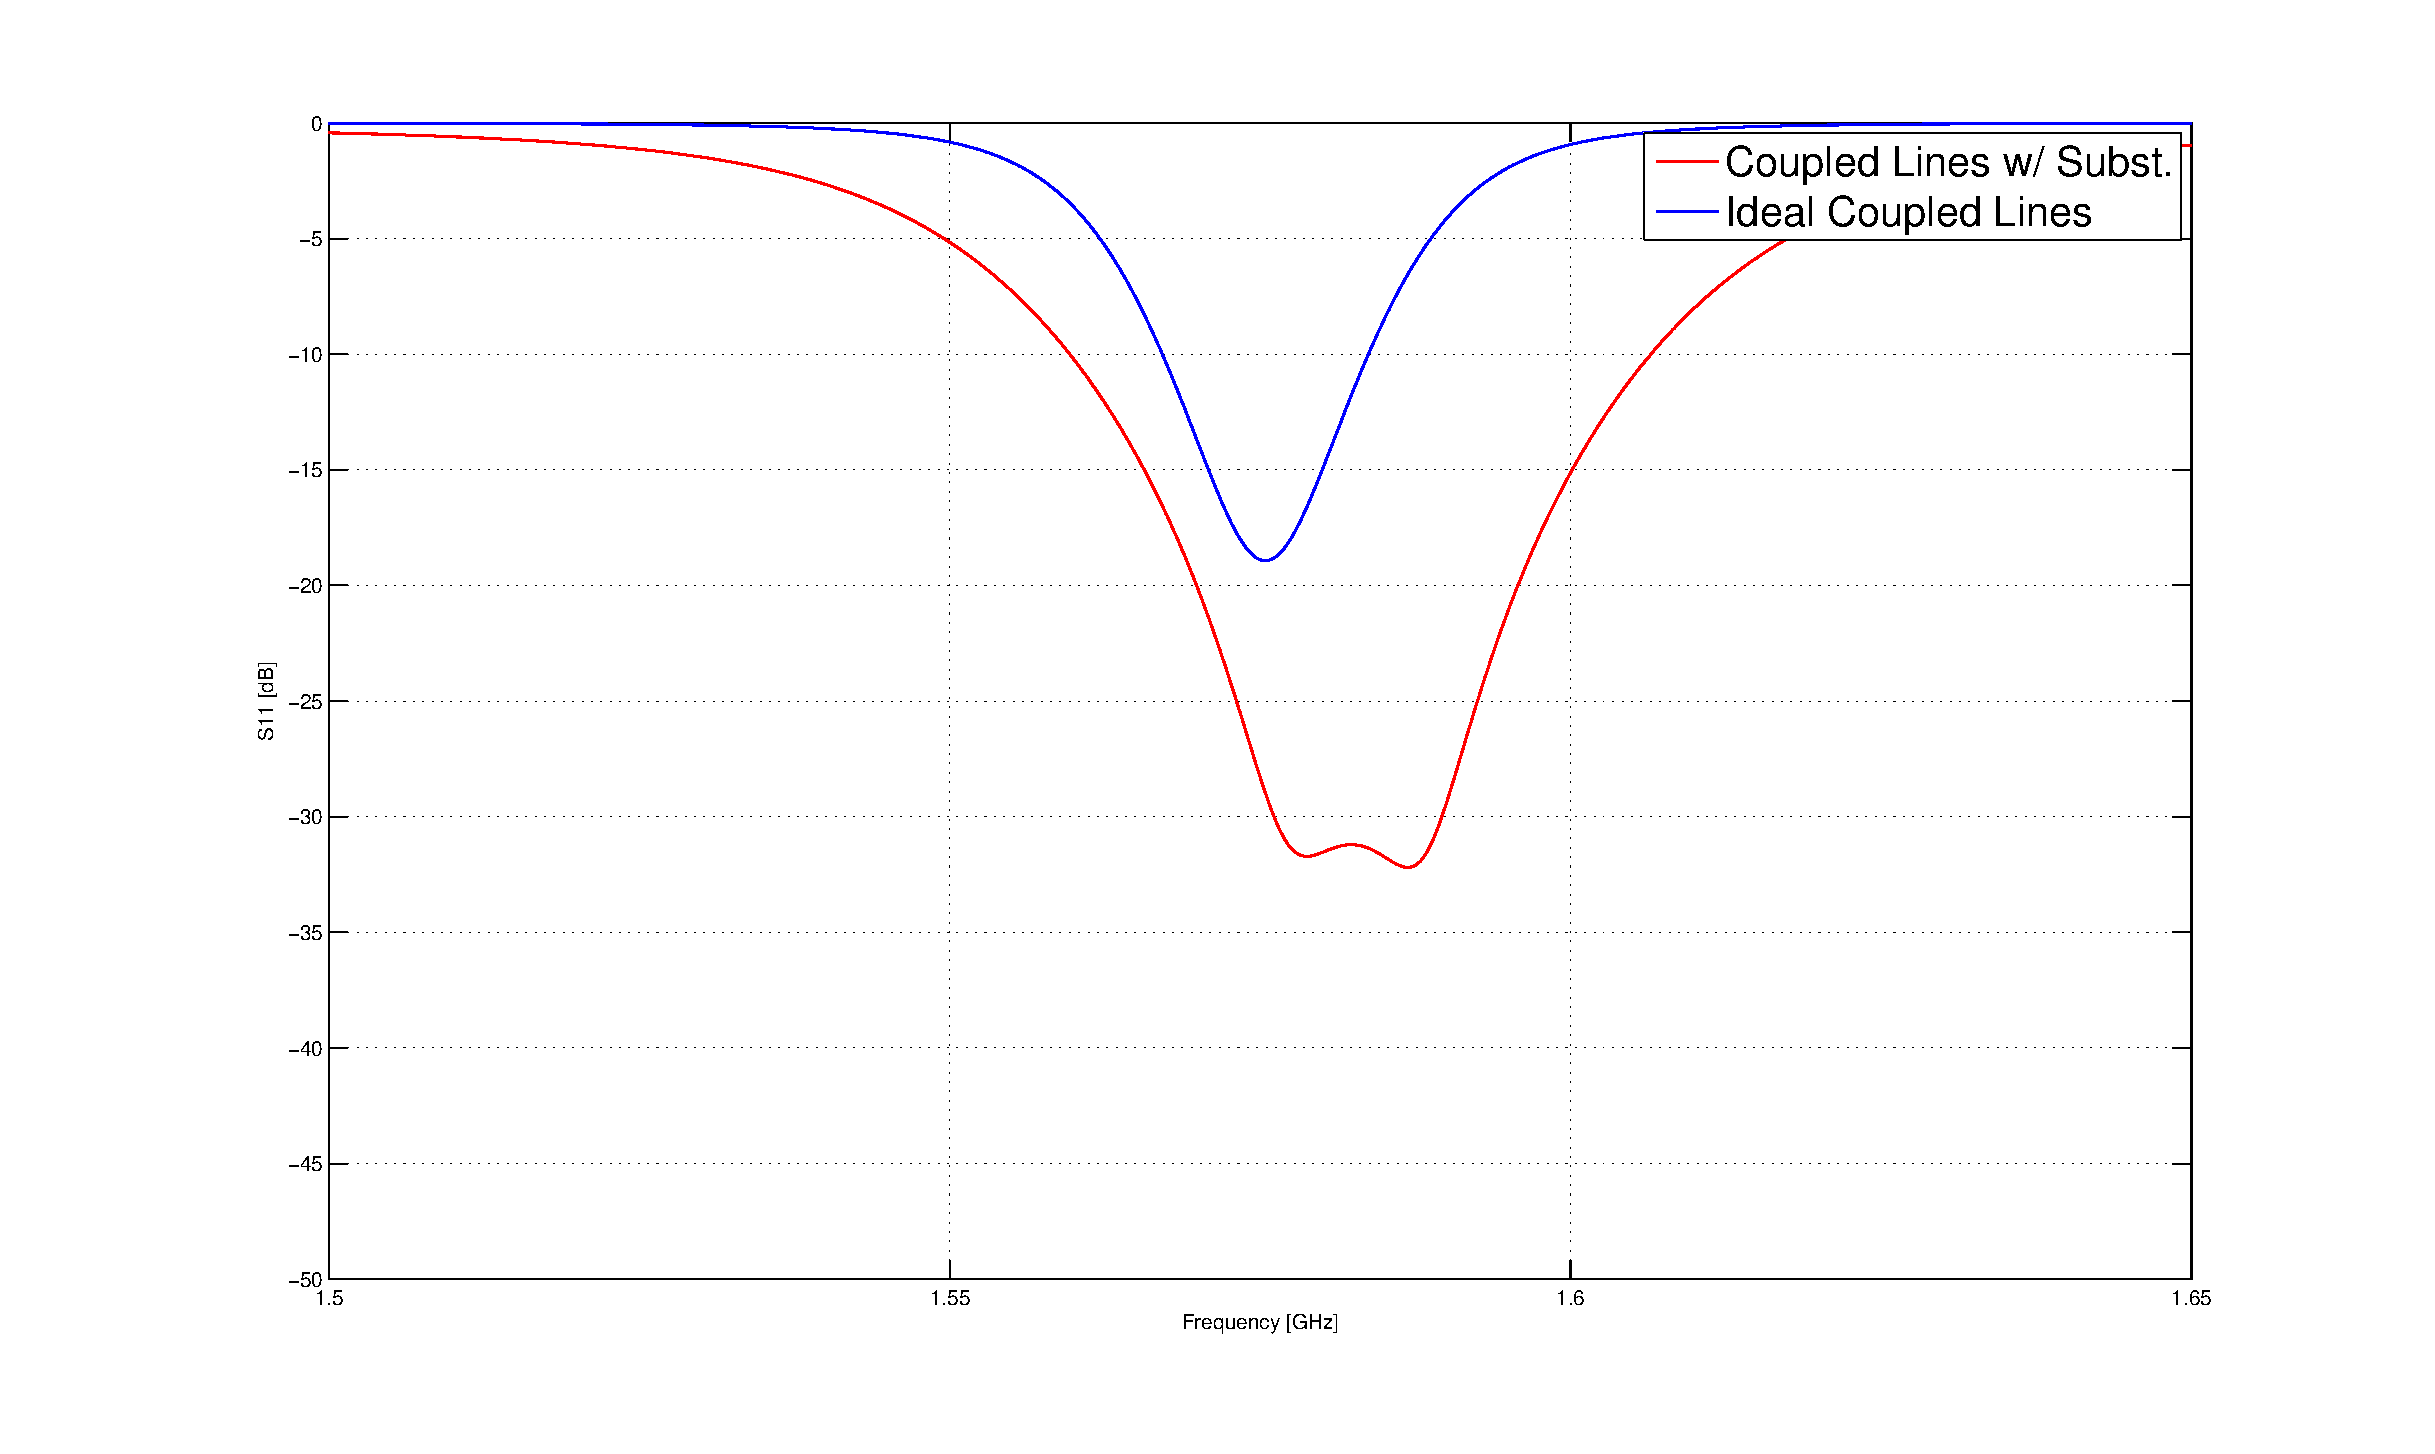
\includegraphics[width=\textwidth]{fig/Filter/2nd_order/plots/S11_subst_CL.eps}
  	\end{subfigure}
  	\begin{subfigure}{0.8\textwidth}
  	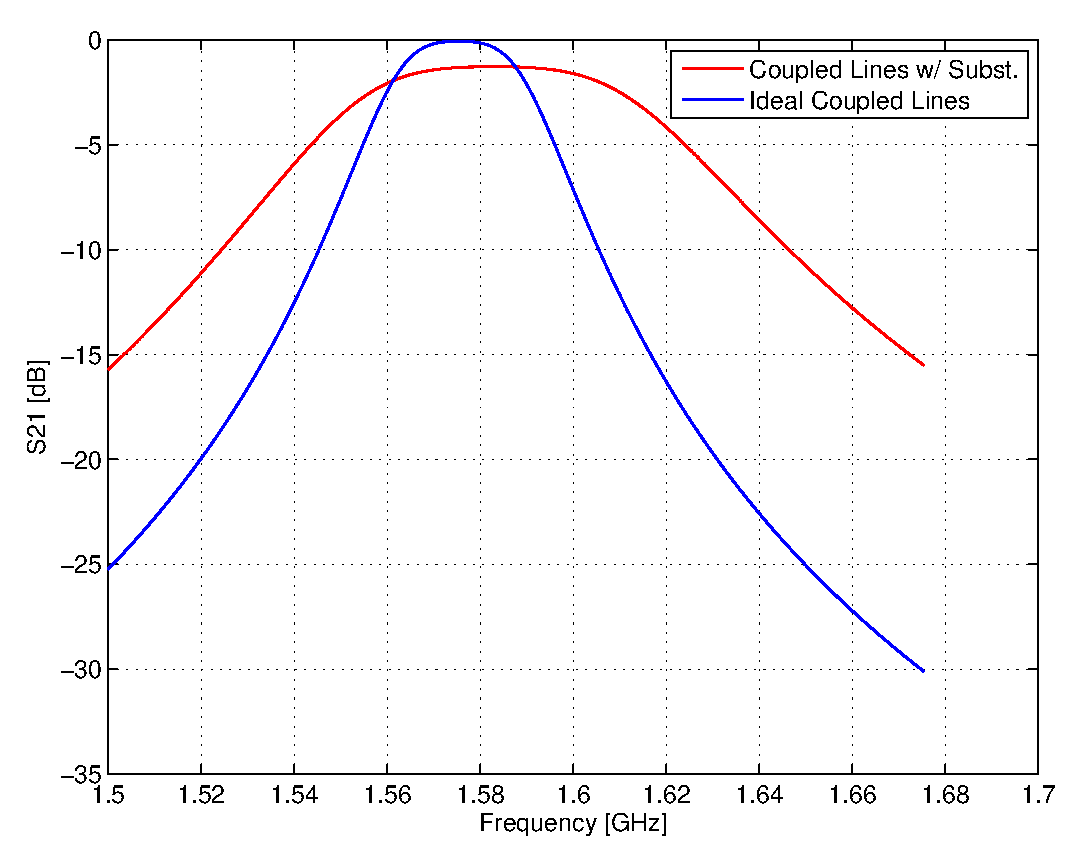
\includegraphics[width=\textwidth]{fig/Filter/2nd_order/plots/S21_subst_CL.eps}
  	\end{subfigure}
  	\caption{S-parameters for CL w/ subst. implementation}
  	\label{fig:filter_spar_subst_CL}
  \end{figure}

\section{Layout}
	\subsection{LNA}
		\subsubsection{Generation of Layout}
			Before generating a layout for the designed LNA circuit, the schematic is made layout friendly. This means the nets in the schematic are replaced by transmission line segments with appropriate impedance, pads for the discrete components are added and discontinuities in microstrip line thickness are modelled in the schematic. After generating a layout from the schematic ground planes are added and vias are placed to connect to the underlying ground plane. A plane for the DC supply voltage is added as well and is placed close to the ground plane for decoupling of the supply voltage, i.e. the small gap acts as a decoupling capacitance. The resulting layout is shown in Figure \ref{fig:lna_layout}. All traces have a width according to an impedance of $\SI{50}{\ohm}$ except for the transmission line in the matching network at the input, which is $\SI{75}{\ohm}$ to reduce the length of the line, and the trace between collector and base as only DC-current flows there. 

			\begin{figure}[H]
			\centering
				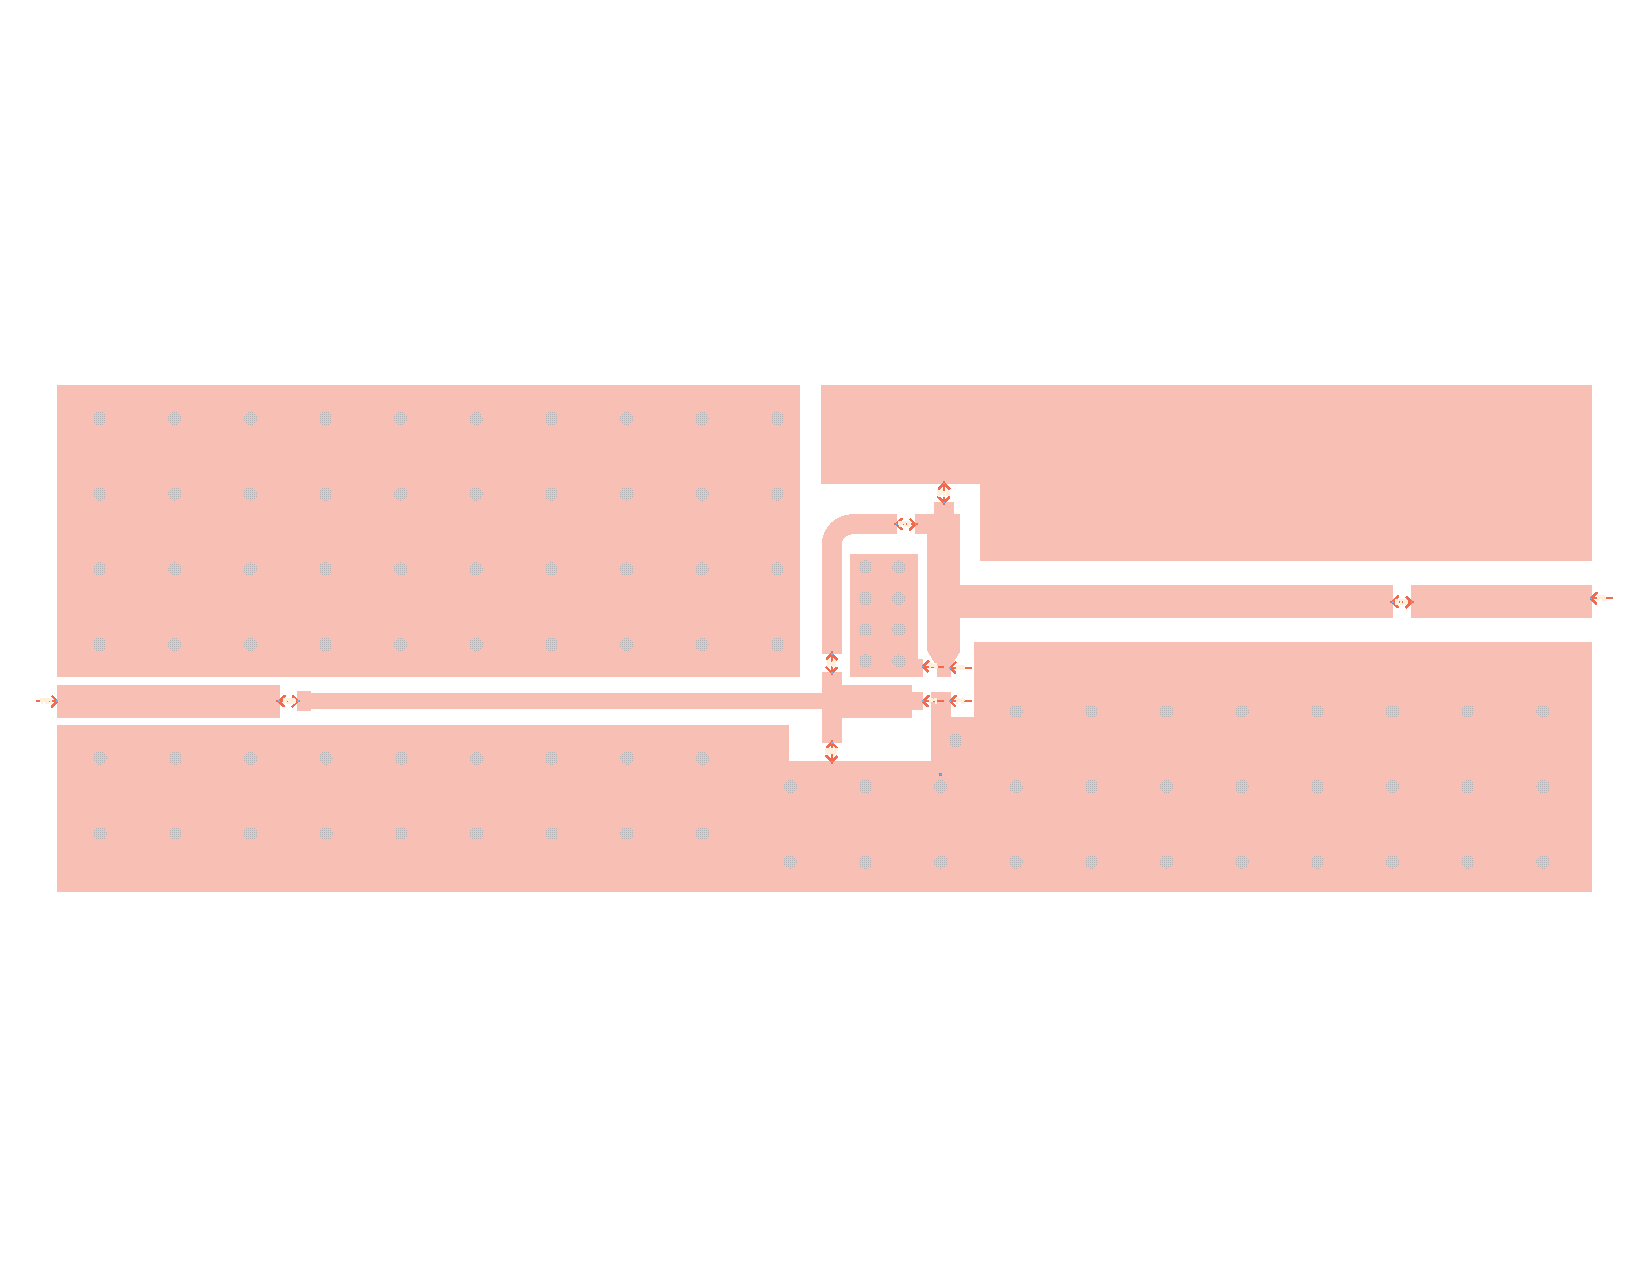
\includegraphics[width=\textwidth]{fig/LNA/LNA_layout.pdf}
				\caption{Generated layout with added ground and source planes}
				\label{fig:lna_layout}
			\end{figure}

		\subsubsection{EM-model Simulations}
			In this step of the design Momentum (full wave) simulations are performed on the drawn layout and an EM-model is generated. This model contains information on transmission line effects, radiation losses, copper losses etc. and can be used to conduct further simulations to better predict the performance of the fabricated device and investigate the differences with the schematic. \\

			The Smith Chart in Figure \ref{fig:lna_smith_post} shows that with inclusion of the EM-model there is a very small mismatch at the input, but the $S_{11}$ is $\SI{-22}{\decibel}$ which is very much acceptable.

			\begin{figure}[H]
			\centering
				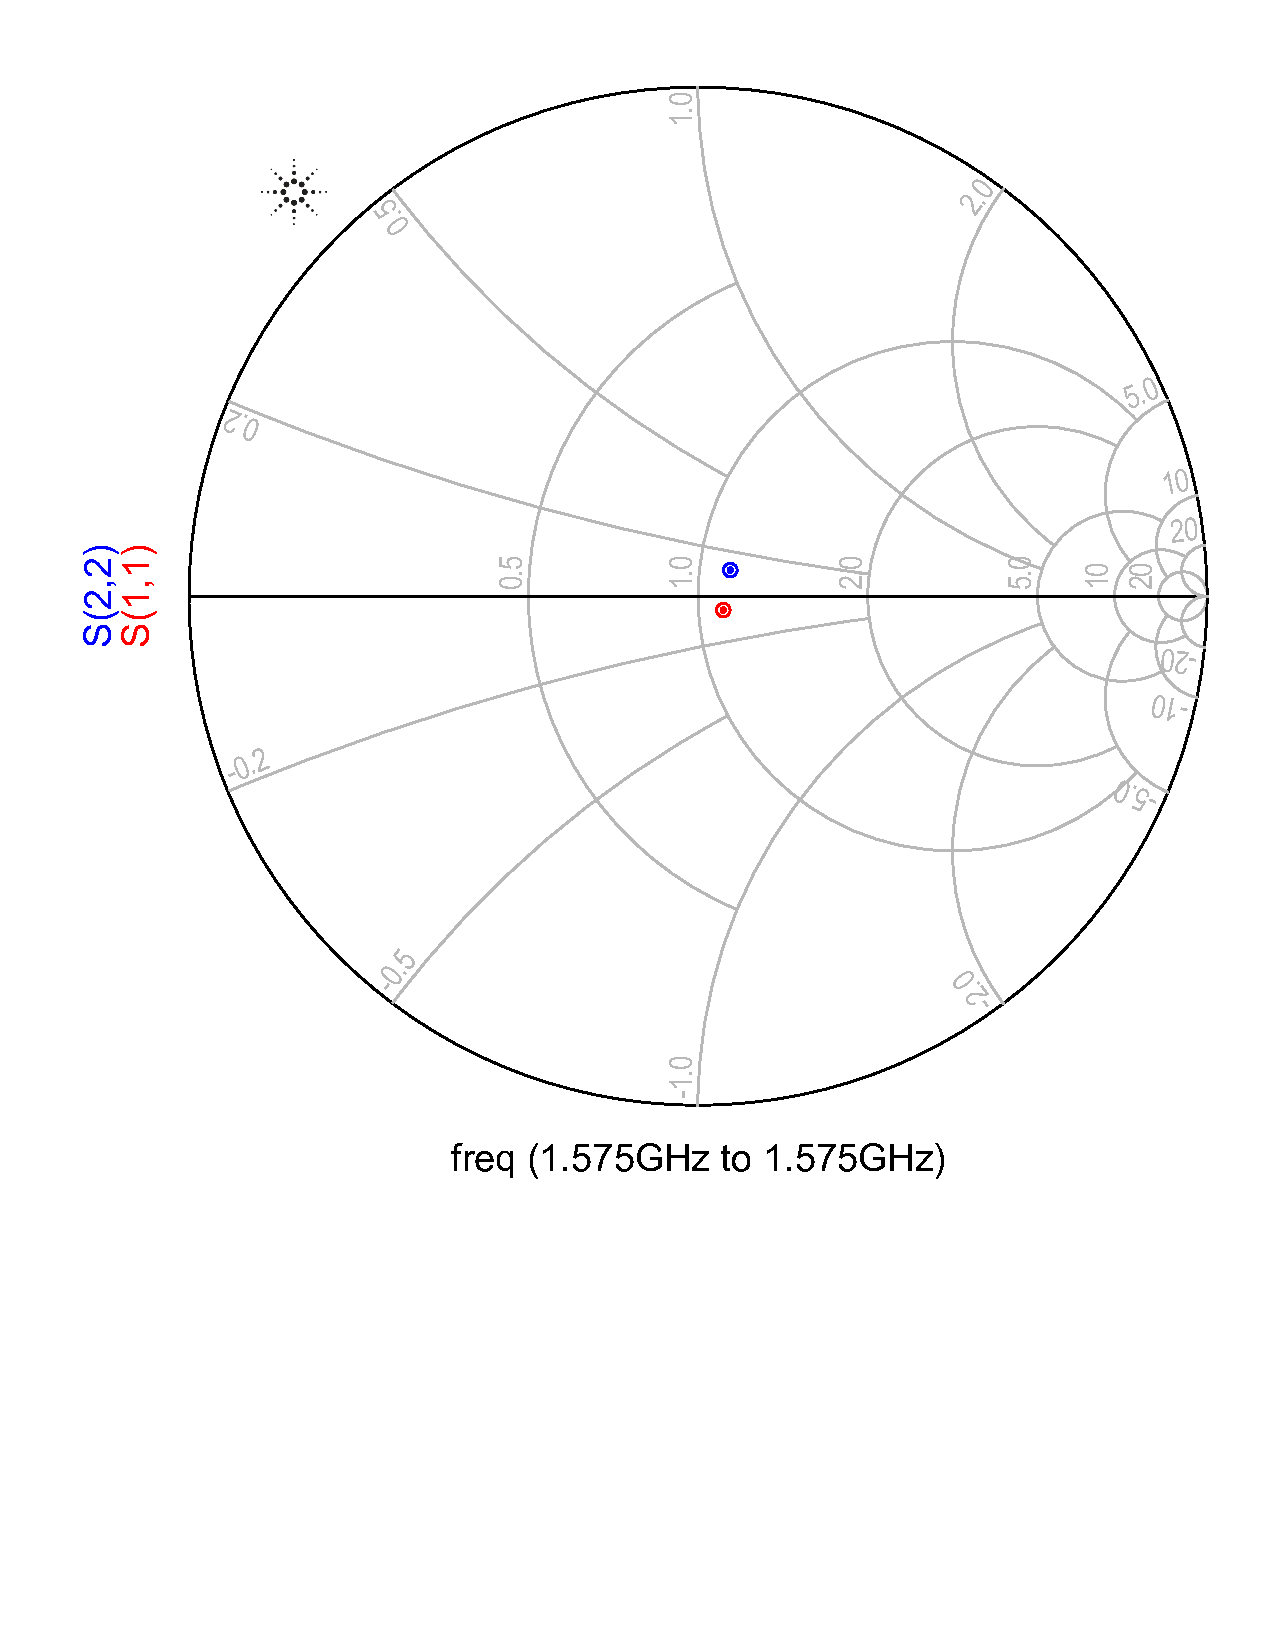
\includegraphics[width=0.5\textwidth]{fig/LNA/matching_post.pdf}
			\caption{Smith Chart with EM-model}
			\label{fig:lna_smith_post}
			\end{figure}

			If we look at the 1-dBCP in Figure \ref{fig:lna_1db_post} we see that the input referred 1-dBCP has increased with $\SI{1}{\dbm}$, but the gain has dropped with approximately the same amount. We get an output referred 1-dBCP of $\SI{4.37}{\dbm}$, which is very close to the value obtained with the schematic ($\SI{4.5}{\dbm}$). 

			\begin{figure}[H]
			\centering
				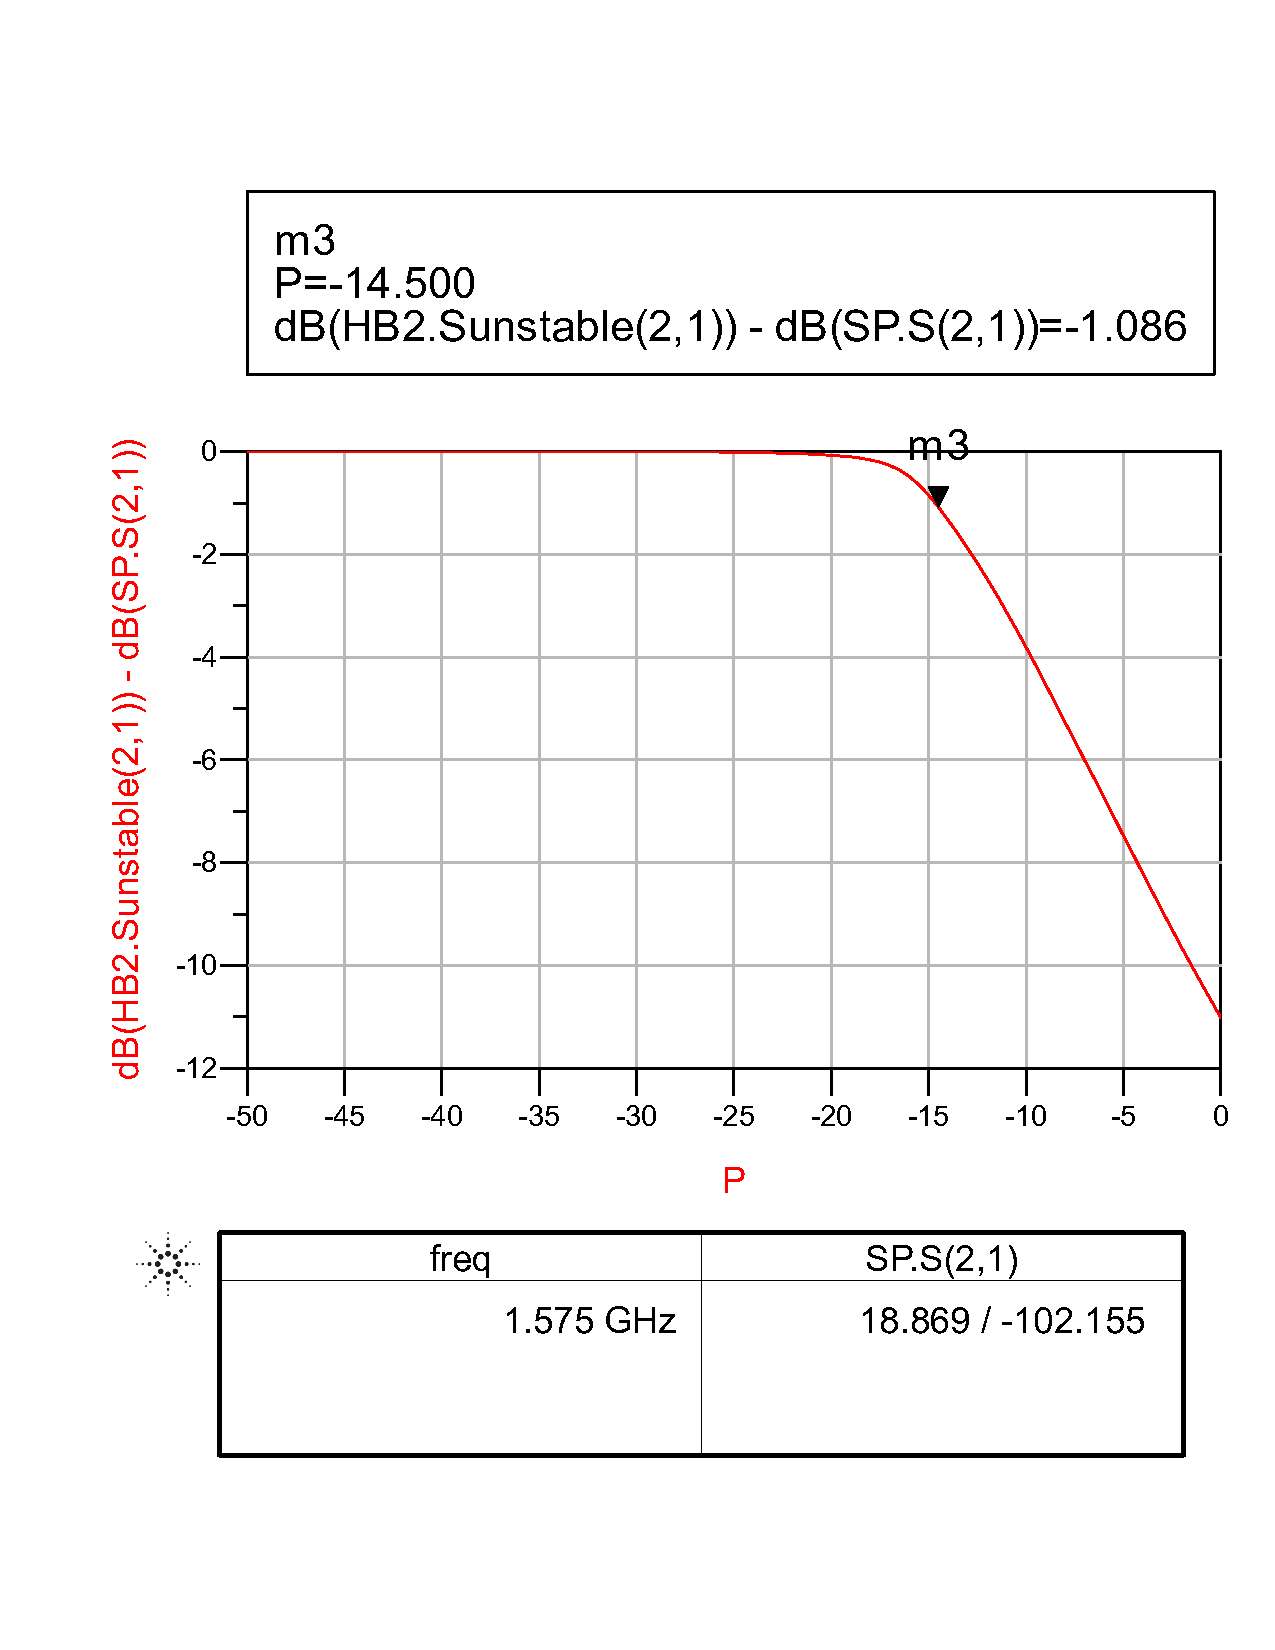
\includegraphics[width=0.5\textwidth]{fig/LNA/compression_post.pdf}
			\caption{1 dB Compression Point with EM-model}
			\label{fig:lna_1db_post}
			\end{figure}

		\subsubsection{Summary}

			\begin{table}[H]
			\centering
			\begin{tabular}{|l|r|r|r|}
				\hline
				 &  \textbf{EM-model} &  \textbf{Schematic} & \textbf{Specs} \\
				\hline
				\textbf{SS Gain} & 18.87 dB &  20 dB & $>$ 16 dB \\
				\hline
				\textbf{NF} & 1.412 dB & 1.196 dB & $\leq$ 1.5 dB \\
				\hline
				\textbf{Output ref. 1dBCP} & 4.37 dBm & 4.5 dBm & $>$ 3 dBm \\
				\hline
				\textbf{FOM} & 0.503 & 0.33 & Max. \\
				\hline
			\end{tabular}
			\caption{Summarizing achieved specs after EM-model simulation}
			\label{tab:lna_em_summ}
			\end{table}


	\subsection{Filter}
		\subsubsection{Generated Layout}
			The generated layout is shown in Figure \ref{fig:filter_layout}. The dimensions are $\SI{1}{\centi\meter}$ by $\SI{9}{\centi\meter}$, which yields an area of $\SI{9}{\centi\meter\squared}$. 

			\begin{figure}[H]
			\centering
				
\includegraphics[width=\textwidth]{fig/Filter/2nd_order/layout.pdf}
				\caption{Generated layout CL filter}
				\label{fig:filter_layout}
			\end{figure}
		
		\subsubsection{EM-model Simulations}
			After generation of the layout an EM-model is extracted and the obtained S-parameters are shown in Figure \ref{fig:filter_em_model}. The attenuation in the passband is $\SI{1.8}{\decibel}$, which is still within the specification of $\SI{2}{\decibel}$ and the bandwidth is approximately $\SI{50}{\mega\hertz}$.

			\begin{figure}[H]
			\centering
				\begin{subfigure}{0.8\textwidth}
				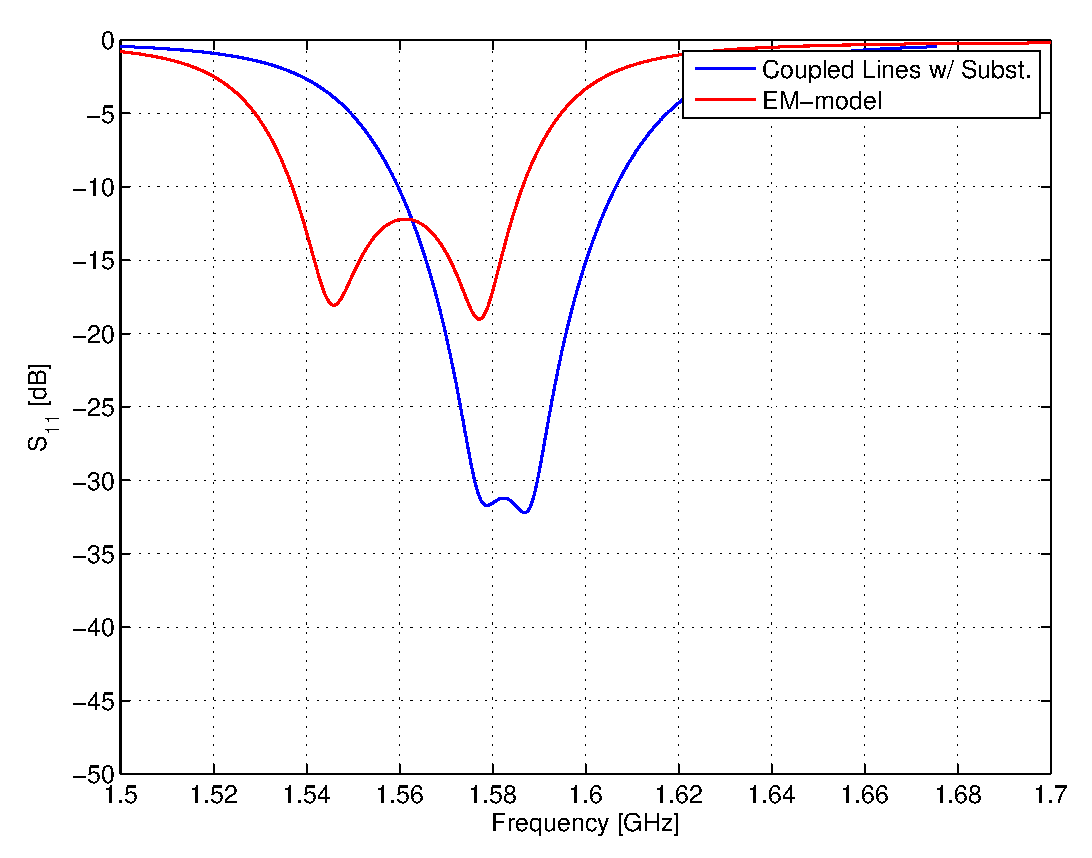
\includegraphics[width=\textwidth]{fig/Filter/2nd_order/plots/S11_layout.eps}
				\end{subfigure}
				\begin{subfigure}{0.8\textwidth}
				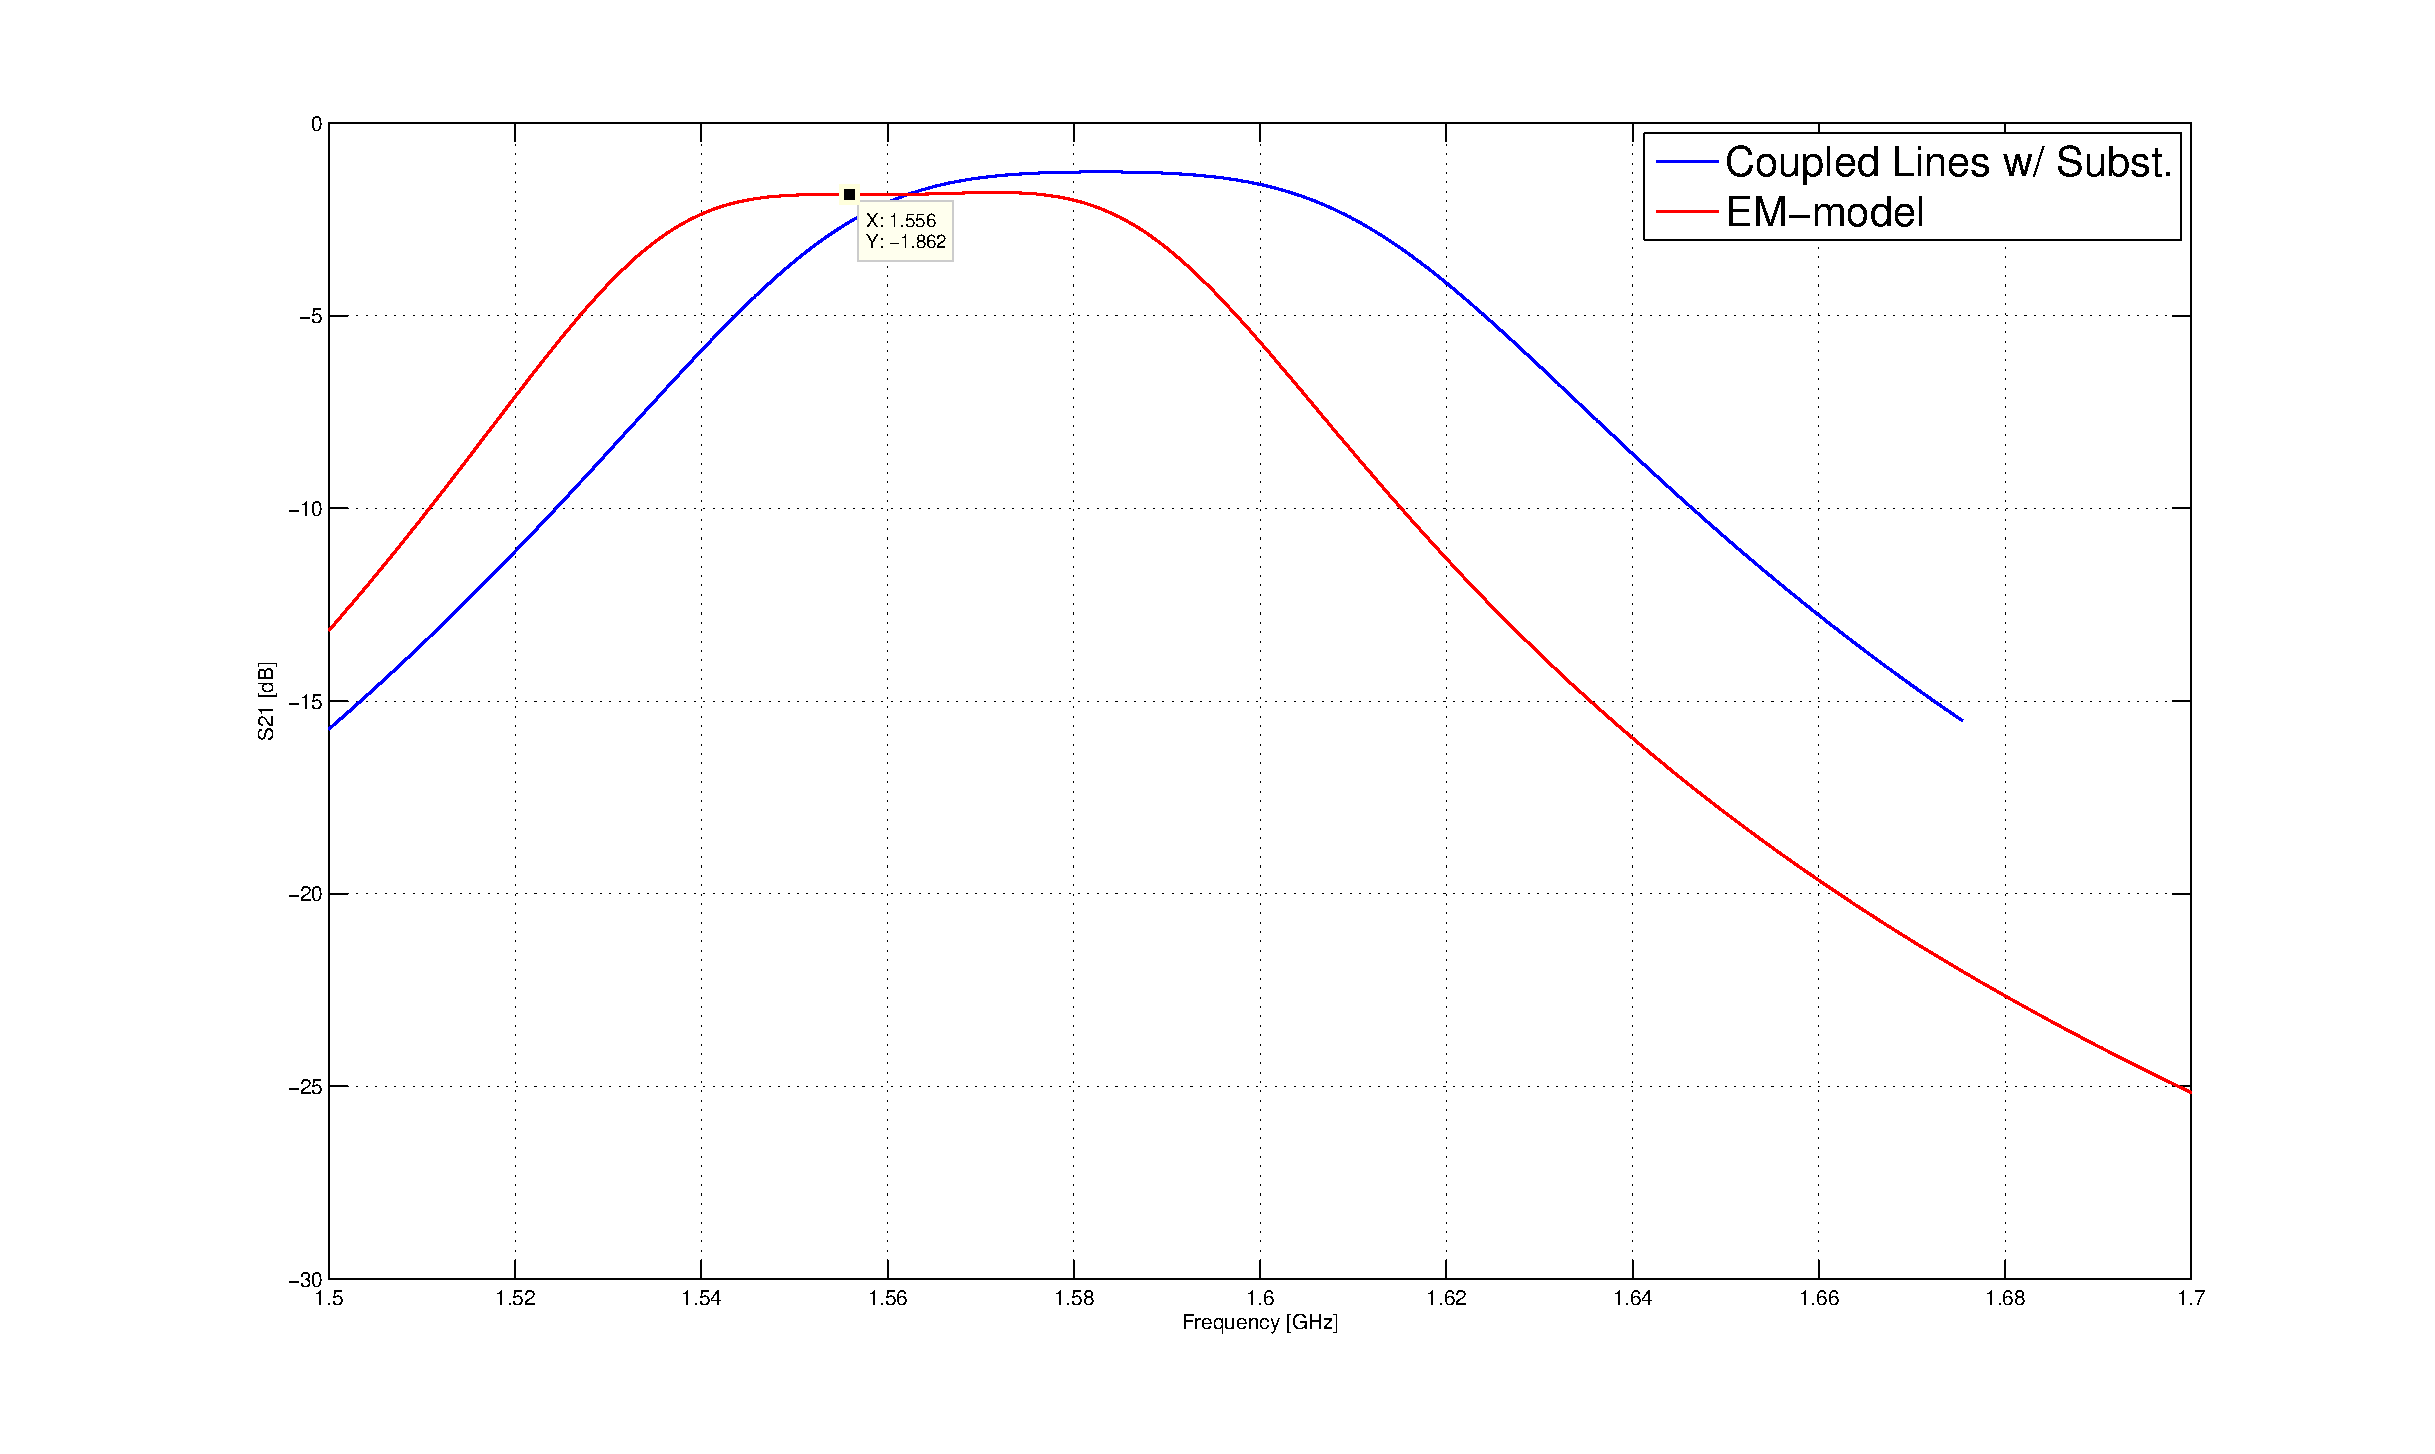
\includegraphics[width=\textwidth]{fig/Filter/2nd_order/plots/S21_layout.eps}
				\end{subfigure}
			\caption{S-parameters for EM-model simulations}
			\label{fig:filter_em_model}
			\end{figure} 
\section{Results}
	\subsection{LNA}
  \subsubsection{S-Parameters}
  \label{sub:sparams}
  We start by measuring the $S_{11}$ and $S_{21}$ and compare with the simulations.
  \autoref{fig:lna_meas_s21} shows a final gain of $\SI{19.45}{\dbm}$ at the central frequency of $\SI{1575.42}{\mega\hertz}$, which is in line with the simulation results in \autoref{tab:lna_em_summ}.
  Also, the $\SI{-10}{\decibel}$ bandwidth is well over the specified $\SI{2.046}{\mega\hertz}$, as \autoref{fig:lna_meas_s11} indicates.
  \begin{figure}[H]
    \centering
    \begin{subfigure}{0.5\textwidth}
      \centering
      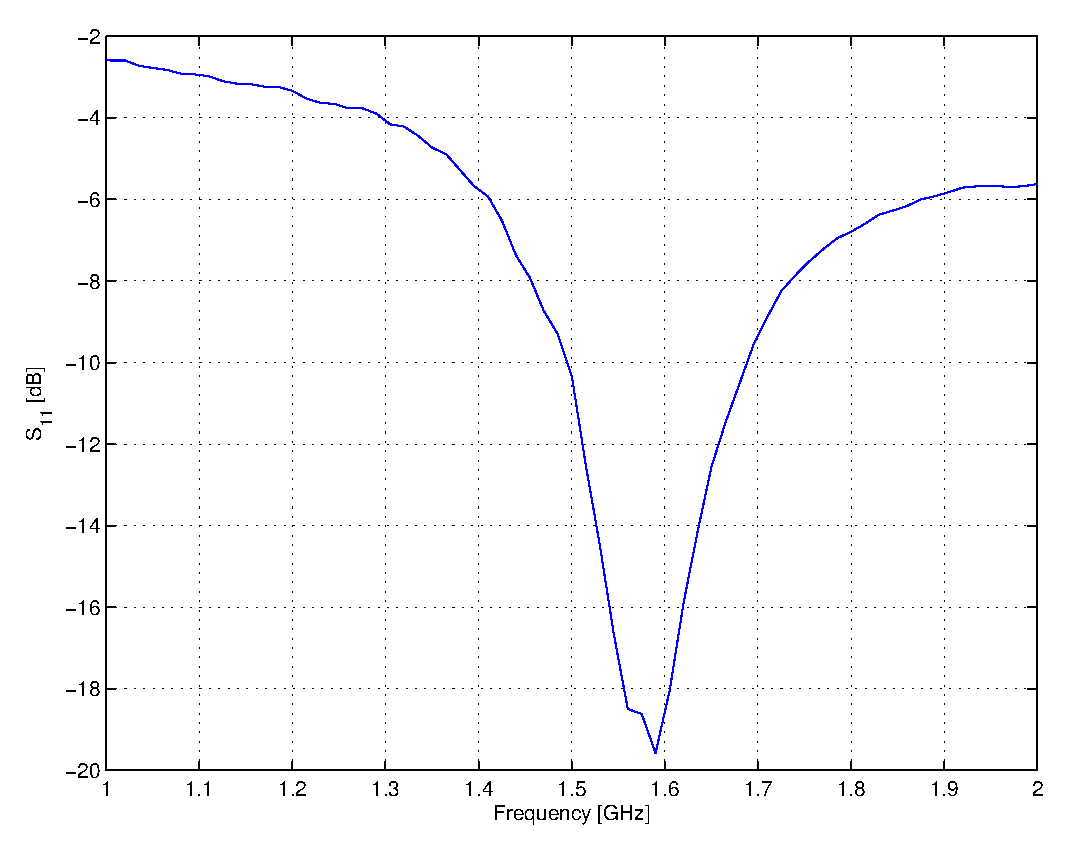
\includegraphics[width=\textwidth]{fig/LNA/s11_lna.eps}
      \caption{Reflection}
      \label{fig:lna_meas_s11}
    \end{subfigure}%
    \begin{subfigure}{0.5\textwidth}
      \centering
      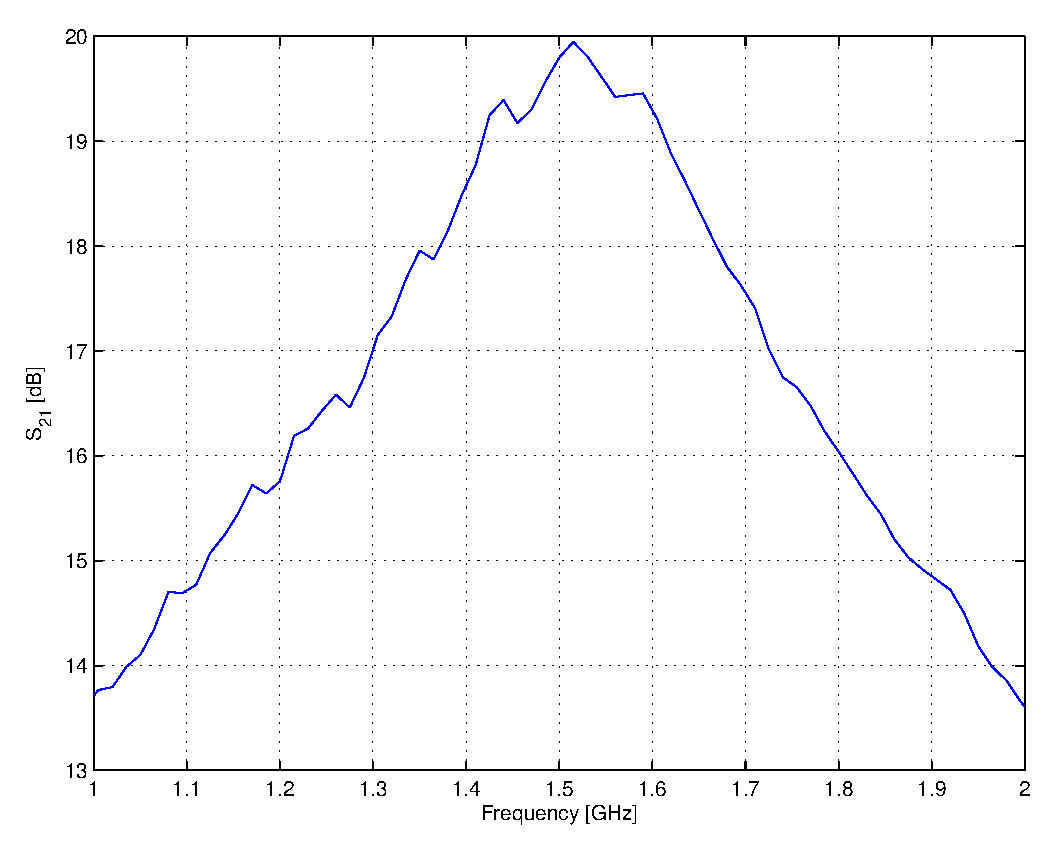
\includegraphics[width=\textwidth]{fig/LNA/s21_lna.eps}
      \caption{Insertion Loss}
      \label{fig:lna_meas_s21}
    \end{subfigure}
    \caption{Measured S-parameters of the LNA}
    \label{fig:lna_meas_sparam}
  \end{figure}
  \subsubsection{$\SI{1}{\decibel}$ Compression Point}
  In order to find the $\SI{1}{\decibel}$ compression point, the output power is measured as a function of the input power, and plotted on \autoref{fig:lna_meas_cp}.
  A curve is fitted to the initial linear part, and the vertical black line indicates the point where the difference between the fitted and measured curve exceeds $\SI{1}{\decibel}$.
  For the tested LNA, this point is at an input power of $\SI{-14}{\dbm}$ and given the gain measured in \autoref{sub:sparams}, this results in an output-referred $\SI{1}{\decibel}$ compression point of $\SI{5.45}{\dbm}$.

  \begin{figure}[H]
    \centering
    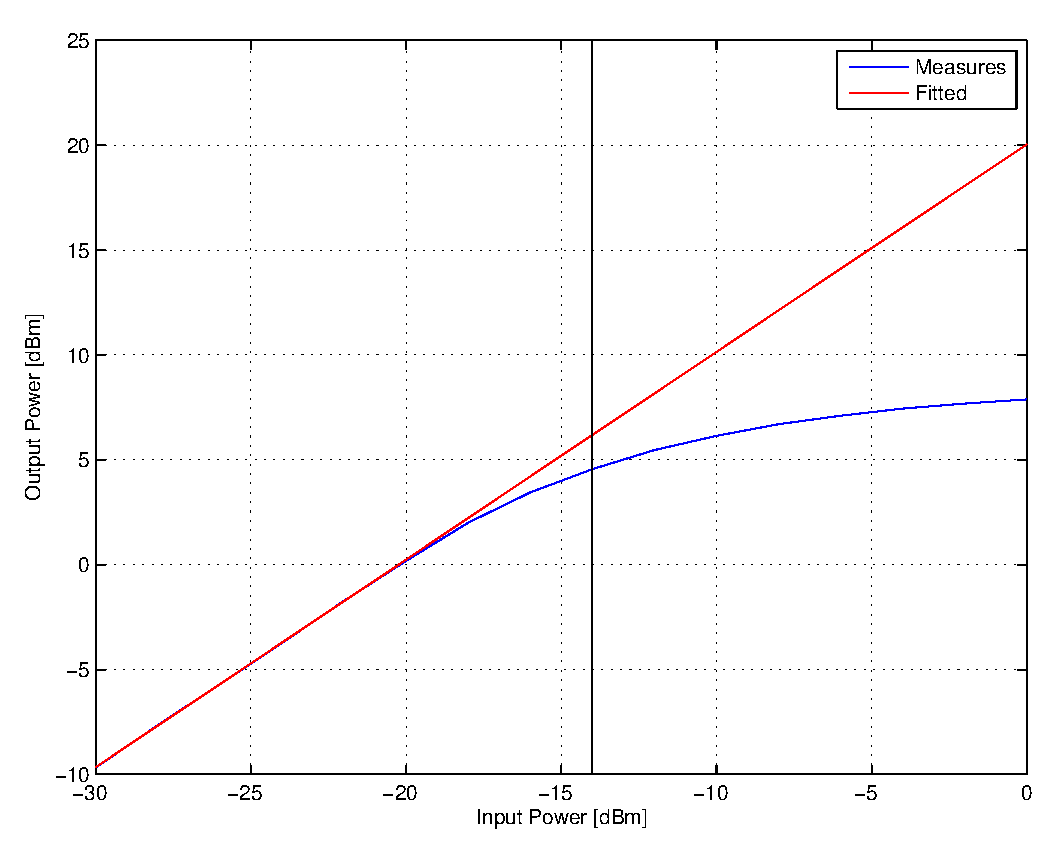
\includegraphics[width=\textwidth]{fig/LNA/compression_lna.eps}
    \caption{Output vs. Input Power}
    \label{fig:lna_meas_cp}
  \end{figure}

  % TODO: Questions from TutorialRFMeasurements
  
  \subsubsection{Harmonic Distortion}
  The test set-up to measure the harmonic distortion consists of two signal generators: one set to $\SI{1575.40}{\mega\hertz}$ (IM-) and the other set to $\SI{1575.44}{\mega\hertz}$ (IM+).
  These inputs will create $3^{rd}$ order intermodulation products at $\SI{1575.36}{\mega\hertz}$ and $\SI{1575.48}{\mega\hertz}$.
  The output power at these four frequencies is then measured for varying input powers, and the lowside and highside measurements are shown in \autoref{fig:lna_meas_im_low} and \autoref{fig:lna_meas_im_high} respectively.
  Once again, lines are fitted to the linear section of the measurements (i.e.\ for input powers \textless $\SI{-14}{\dbm}$).

  \begin{figure}[H]
    \centering
    \begin{subfigure}{0.5\textwidth}
      \centering
      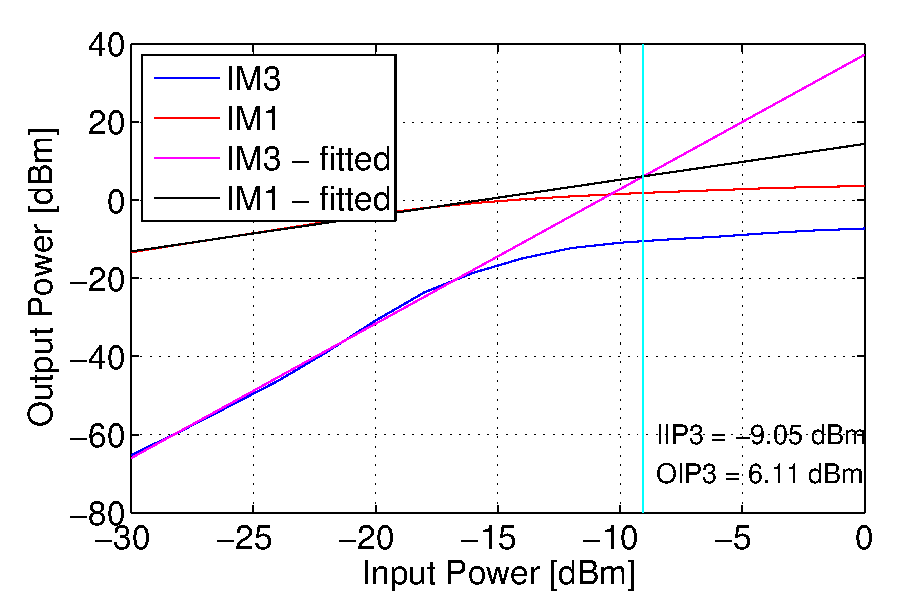
\includegraphics[width=\textwidth]{fig/LNA/im_low_lna.eps}
      \caption{Lowside Intermodulation Products}
      \label{fig:lna_meas_im_low}
    \end{subfigure}%
    \begin{subfigure}{0.5\textwidth}
      \centering
      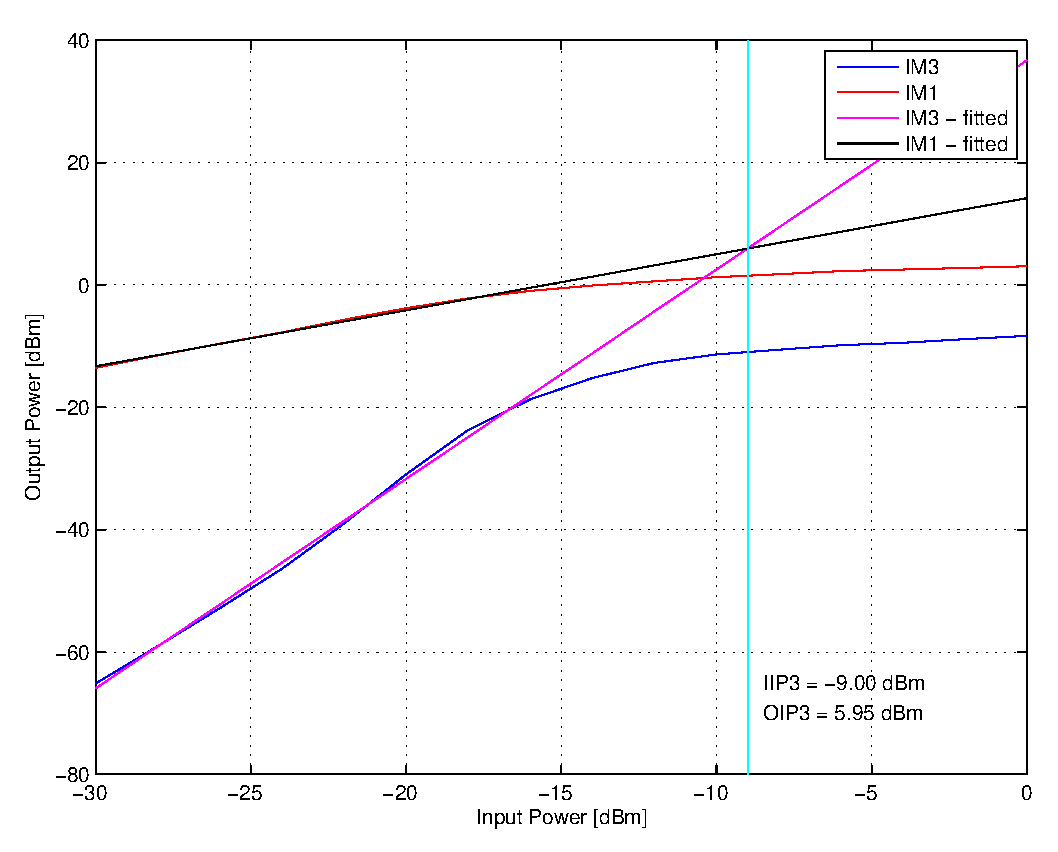
\includegraphics[width=\textwidth]{fig/LNA/im_high.eps}
      \caption{Highside Intermodulation Products}
      \label{fig:lna_meas_im_high}
    \end{subfigure}
    \caption{Measurements for Intermodulation Products}
    \label{fig:lna_meas_im}
  \end{figure}

  In \autoref{fig:lna_meas_im} the vertical lines indicate the intercept points. The OIP3 is found by simply reading the value of the ordinate in both plots. For the final OIP3 we choose the average of both, namely $\SI{6.03}{\dbm}$, however we did not factor in the losses that are introduced by the power combiner used to inject the two tones simultaneously. Hence the OIP3 is $\SI{12}{\dbm}$.

  \subsubsection{Noise}
  To measure the noise, we choose to use the noise figure meter, as it is the most accurate for low noise figures ($\le$ $\SI{2}{\decibel}$).
  We measured a value of $\SI{1.22}{\decibel}$, which is perfectly in line with the simulation result of $\SI{1.196}{\decibel}$ in \autoref{tab:lna_summ} and even better than the EM-simulation result.

  \subsubsection{Figure of merit}
  Finally we measure the power usage of the LNA: at $\SI{5}{\volt}$, a current of $\SI{13}{\milli\ampere}$ is drawn from the power supply, yielding a power consumption of $\SI{65}{\milli\watt}$.
  Combining this value with the OIP3 measured earlier, we find a figure of merit of $0.244$, a value lower than would be expected from simulation.

  One explanation for this would be the lower intercept point: $\SI{12}{\dbm}$ vs. $\SI{16.27}{\dbm}$ from simulation.
  A lower OIP3 would suggest a lower linearity than expected, however the $\SI{1}{\decibel}$ compression point is actually higher than the simulations would indicate.

	\subsection{Filter}
  \autoref{fig:filter_meas_s21} displays the insertion loss of the filter. While we can see that the lowest GSM-1800 frequency of $\SI{1710}{\mega\hertz}$ is attenuated sufficiently, the passband has slightly too much loss.
  The $\SI{-10}{\decibel} S_{11}$ is $\SI{50}{\mega\hertz}$ and thus well over the required specifications. 
  \begin{figure}[H]
    \centering
    \begin{subfigure}{0.5\textwidth}
      \centering
      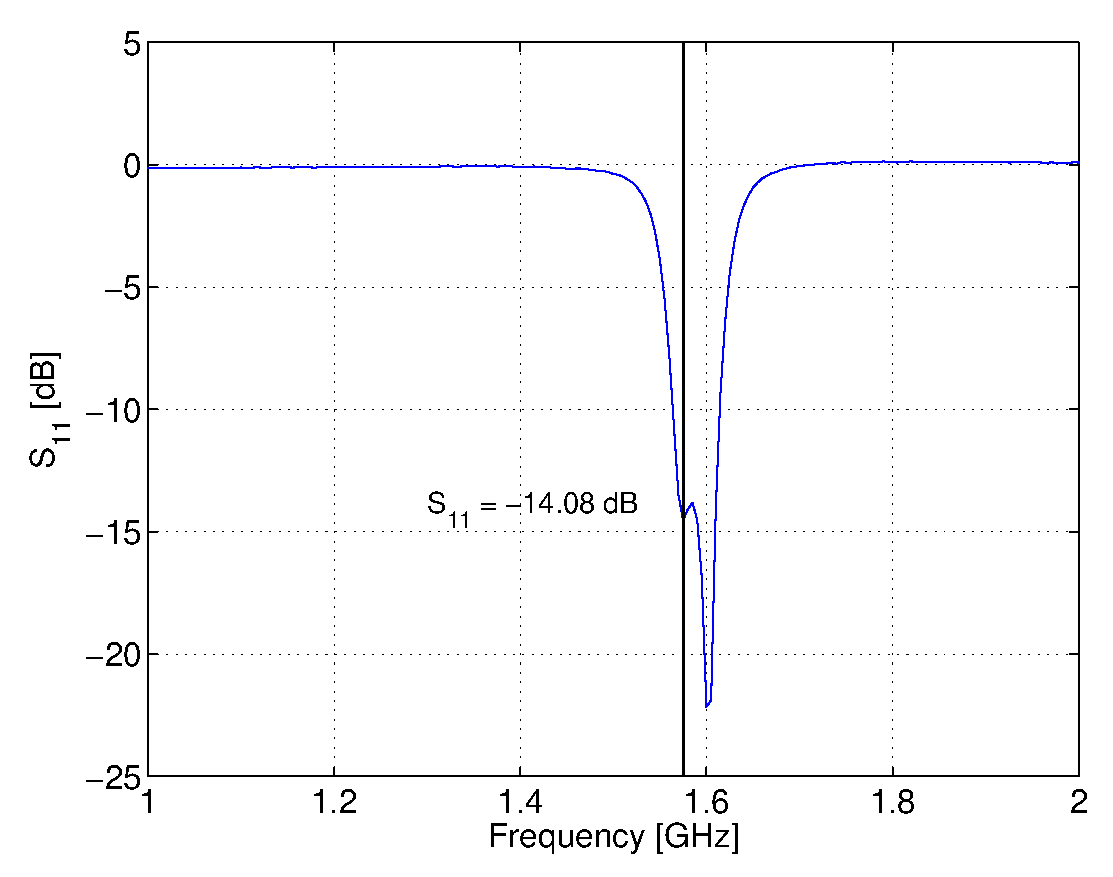
\includegraphics[width=\textwidth]{fig/Filter/s11_filter.eps}
      \caption{Reflection}
      \label{filter_meas_s11}
    \end{subfigure}%
    \begin{subfigure}{0.5\textwidth}
      \centering
      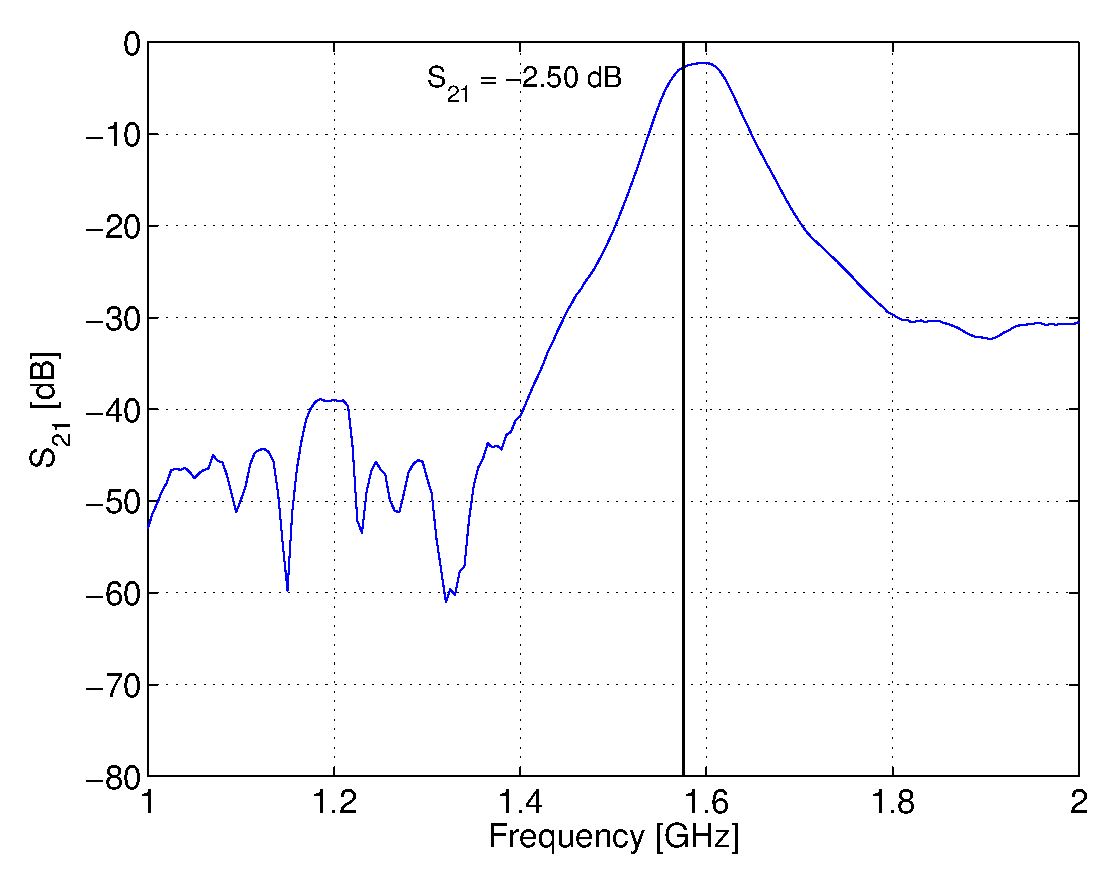
\includegraphics[width=\textwidth]{fig/Filter/s21_filter.eps}
      \caption{Insertion Loss}
      \label{fig:filter_meas_s21}
    \end{subfigure}
    \caption{Measured S-parameters for the filter}
    \label{fig:filter_meas_sparams}
  \end{figure}

  The board measures approx. $\SI{1}{\centi\meter}$ by $\SI{9}{\centi\meter}$, yielding a surface of $\SI{9}{\centi\meter\squared}$, which serves as a Figure of Merit. 

  \subsection{Complete System}
  In order to test the complete system, the filter is placed in front of the LNA, and two tones are injected into the system: one at $\SI{1575.42}{\mega\hertz}$ (i.e.\ the desired signal) and one at $\SI{1710}{\mega\hertz}$ (i.e.\ the disturbance).  
  Both signals have a power of $\SI{-30}{\dbm}$ and the combination of cables and connectors used in the set-up has a loss of approx. $\SI{7}{\dbm}$.
  \autoref{fig:complete_system} shows the GPS signal with an overall amplification of approx. $\SI{15.57}{\decibel}$ ($\SI{-21.43}{\dbm}$ - $\SI{-30}{\dbm}$ - $\SI{-7}{\decibel}$). This is lower than the LNA gain, as there is attenuation from the filter.
  The GSM-disturbance signal is suppressed by approx. $\SI{5.6}{\decibel}$, and is $\SI{21.17}{\decibel}$ smaller than the desired signal, hence we can conclude the system has suppressed the disturbance sufficiently.
  \begin{figure}[H]
    \centering
    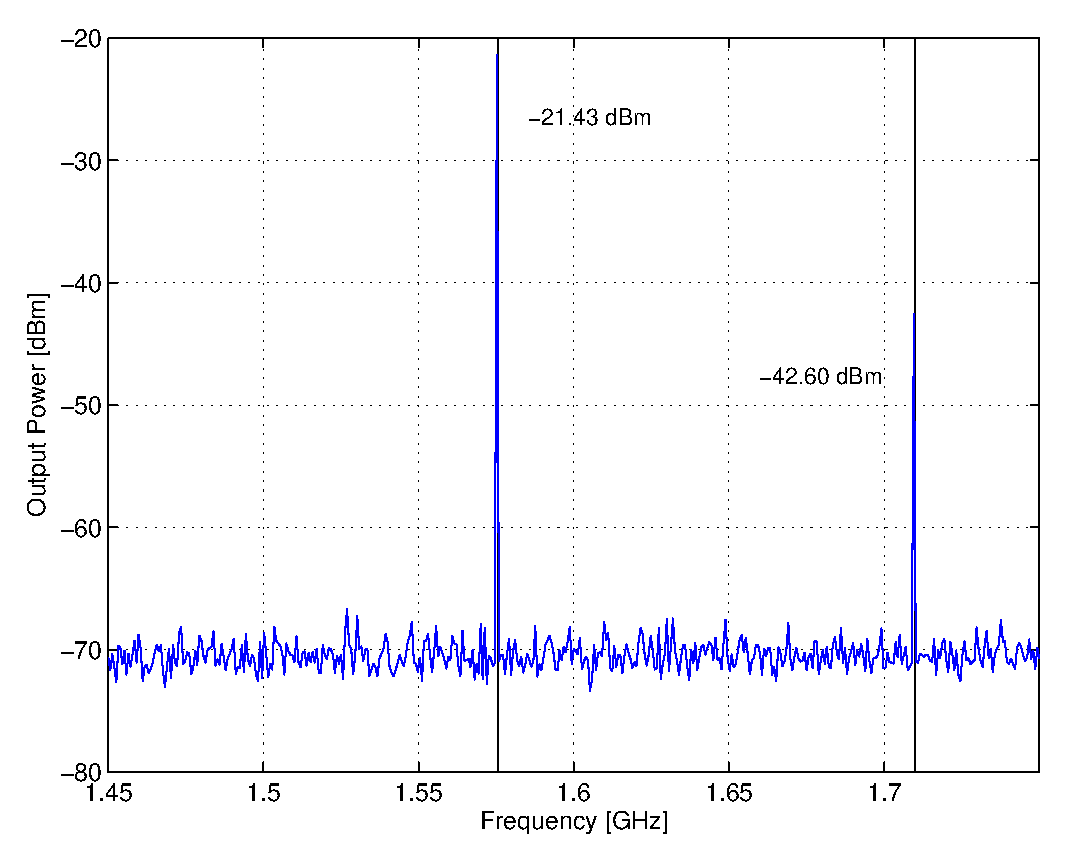
\includegraphics[width=\textwidth]{fig/Filter/spectrum_system.eps}
    \caption{Spectrum of complete system}
    \label{fig:complete_system}
  \end{figure}
\section{Conclusion}

\section{Further improvements}

	\subsection{LNA}

	\subsection{Filter}
		A first improvement to the filter would be to decrease the bandwidth. The specifications state that a bandwidth of $\SI{2}{\mega\hertz}$ is needed, but we achieved $\SI{50}{\mega\hertz}$, which is well overdimensioned. As there always is a trade off between bandwidth and noise, a smaller bandwidth would be better for noise considerations. \\

		Secondly, the attenuation in the passband could be improved, as it is the only specification that hasn't been met: $\SI{2.5}{\decibel}$ instead of the desired maximum of $\SI{2}{\decibel}$. This could be done by decreasing the attenuation even further in the simulation by means of shorter transmission lines or smaller gaps between the TLs, as this will result in more coupling, while still meeting the other specifications. Hence, it will be a complicated optimization. \\

		Thirdly, as the area of the filter is used as a FOM, it could be made smaller by folding the coupled lines. 

\bibliographystyle{plain}
\bibliography{bookref}
\end{document}
